
\documentclass[msc,lith,english,hidelinks]{liuthesis}

%% Settings go in settings.tex


\usepackage[backend=biber, sorting=none, hyperref]{biblatex}
%% To set the font of your thesis, use the \setmainfont{} command,
%% surrounded with \ifxetex if you want to switch between xelatex and pdflatex
\ifxetex 
%\setmainfont [Scale=1]{Georgia}
\fi

%%%%%%%%%%%%
%% The VZ43 chapter style, from Memoir contributed chapter styles: ftp://ftp.tex.ac.uk/ctan%3A/info/MemoirChapStyles/MemoirChapStyles.pdf
%%%%%%%%%%%

\usepackage{calc,color}
\newif\ifNoChapNumber
\newcommand\Vlines{%
\def\VL{\rule[-2cm]{1pt}{5cm}\hspace{1mm}\relax}
\VL\VL\VL\VL\VL\VL\VL}
\makeatletter
\setlength\midchapskip{0pt}
\makechapterstyle{VZ43}{
\renewcommand\chapternamenum{}
\renewcommand\printchaptername{}
\renewcommand\printchapternum{}

\renewcommand\chapnumfont{\Huge\bfseries\centering}
\renewcommand\chaptitlefont{\Huge\bfseries\raggedright}
\renewcommand\printchaptertitle[1]{%
\Vlines\hspace*{-2em}%
\begin{tabular}{@{}p{1cm} p{\textwidth-3cm}}%
\ifNoChapNumber\relax\else%
\colorbox{black}{\color{white}%
\makebox[.8cm]{\chapnumfont\strut \thechapter}}
\fi
& \chaptitlefont ##1
\end{tabular}
\NoChapNumberfalse
}
\renewcommand\printchapternonum{\NoChapNumbertrue}
}
\makeatother


%% To set bibliography options, refer to the biblatex manual and use
%% the ExecuteBibliographyOptions command below to set your options

\ExecuteBibliographyOptions{maxnames=99}


%% Change this to your appropriate BibTeX reference file (.bib)

\addbibresource{references.bib}

 

\usepackage{rotating}
\usepackage{color, soul}
\usepackage{acro}
\usepackage{longtable} 
%\usepackage[bookmarksnumbered=true]{hyperref}
\usepackage{bookmark}% http://ctan.org/pkg/bookmark
\bookmarksetup{depth=3}
\usepackage{float}
\usepackage[skip=0cm,list=true]{subcaption}
\usepackage{listings}
%\usepackage{background}
%\usepackage{todonotes}
\usepackage{mathtools}
\usepackage{amsthm}
\usepackage{bm}
\usepackage{fontspec}
\setmonofont{Consolas}[Scale=0.85]

\newtheorem{definition}{Definition}[section]
\theoremstyle{remark}
\newtheorem{property}{Property}

\setcounter{secnumdepth}{4}

\usepackage{enumitem}
\setlist{noitemsep} % or \setlist{noitemsep} to leave space around whole list

\department{Institutionen för datavetenskap}
\departmentenglish{Department of Computer and Information Science}
\departmentshort{IDA}

\titleenglish{Reduction of Power Supply Units Hardware Alarms in Radio Base Stations using Machine Learning}
% \subtitleenglish{}
\titleswedish{}
\thesissubject{Statistics and Machine Learning}
\publicationyear{2021}
\currentyearthesisnumber{048}
\dateofpublication{2021-09-14}

\author{Agustín Valencia González}
\supervisor{Sanjiv Dwivedi}
\examiner{Oleg Sysoev}
\externalsupervisor{Oleg Gorbatov, Lackis Eleftheriadis}
\dedication{To Ana María.}

%% Watermark setup
%\backgroundsetup{
%	contents=DRAFT,
%	color=gray!30,
%	scale=15
%}

%% Code styling
\lstset
{ %Formatting for code in appendix
	xleftmargin=1cm,
	numbers=left,
	breaklines=true,
	breakatwhitespace=false,
	frame=single,
	basicstyle=\ttfamily,
}

%% Glossary setup
%% Manual : http://ctan.math.washington.edu/tex-archive/macros/latex/contrib/acro/acro-manual.pdf


\DeclareAcronym{rbs}{
	short = RBS,
	long = Radio Base Station
}

\DeclareAcronym{ru}{
	short = RU, 
	long = Radio Unit
}

\DeclareAcronym{psu}{
	short = PSU, 
	long = Power Supply Unit
}

\DeclareAcronym{oss}{
	short = OSS, 
	long = Operations Support System
}

\DeclareAcronym{noc}{
	short = NOC, 
	long = Network Operations Centre 
}

\DeclareAcronym{pdu}{
	short = PDU, 
	long = Power Distribution Unit 
}

\DeclareAcronym{mcar}{
	short = MCAR, 
	long = Missing Completely at Random
}

\DeclareAcronym{mae}{
	short = MAE, 
	long = Mean Absolut Error
}

\DeclareAcronym{obe}{
	short = OBE, 
	long = Out-of-Bounds Error
}

\DeclareAcronym{mobe}{
	short = MOBE, 
	long = Mean Out-of-Bounds Error
}

\DeclareAcronym{aic}{
	short = AIC, 
	long = Akaike Information Criterion
} 

\DeclareAcronym{gam}{
	short = GAM, 
	long = Generalized Additive Model
} 

\DeclareAcronym{rmse}{
	short = RMSE, 
	long = Root Mean Square Error
}

\DeclareAcronym{svr}{
	short = SVR, 
	long = Support Vector Regression
}

\DeclareAcronym{mlp}{
	short = MLP, 
	long = Multi-Layer Perceptron
}

\DeclareAcronym{lstm}{
	short = LSTM, 
	long = Long Short-Term Memory
}

\DeclareAcronym{rf}{
	short = RF, 
	long = Random Forest
}
 
\DeclareAcronym{eennp}{
 	short = EENNP, 
 	long = Evolutionary Ensemble Neural Network Pool
}

\DeclareAcronym{gru}{
	short = GRU, 
	long = Gated Recurrent Unit
}

\DeclareAcronym{critic}{
	short = CRITIC, 
	long = Criteria Importance Through Intercriteria Correlation
}

\DeclareAcronym{mno}{
	short = MNO, 
	long = Mobile Network Operator
}

\DeclareAcronym{3gpp}{
	short = 3GPP, 
	long = 3rd Generation Partnership Project
}

\DeclareAcronym{mcmc}{
	short = MCMC, 
	long = Markov Chain Monte Carlo
}


\DeclareAcronym{hmc}{
	short = HMC, 
	long = Hamiltonian Monte Carlo
}

\DeclareAcronym{nuts}{
	short = NUTS, 
	long = no-U-turn sampler
}

\DeclareAcronym{api}{
	short = API, 
	long = Application Programable Interface
}


\DeclareAcronym{gbt}{
	short = GBT, 
	long = Gradient Boosting Tree
}

\acsetup {
 make-links = true,
 index/use = true, 
 list/template = longtable,
 list/display = all,
 pages/display = first,
 pages/seq/use = true,
 pages/fill = \acrodotfill,
 pages/name = true
}


%\setuptodonotes{
%	tickmarkheight=0.3cm,
%	color=green!40
%}
\setcounter{secnumdepth}{4}

\begin{document}


\chapterstyle{VZ43}

% Reset the acronym counts since the abstract already counts some
\acresetall


\chapter{Introduction}
\label{cha:introduction}

\section{Motivation}

\subsection{Context}

Mobile communication have shaped how people interact with each other in modern societies. Therefore, it is valid to state that mobile networks are fundamental building blocks for modern lifestyles. Usually, its infrastructure underlies silent and unnoticed. Nonetheless, when they stop working as expected, unpleasant situations, and even chaotic ones, can happen.

Usually, the most visual element of mobile networks for the common eye is the antenna towers. Although, there are several more components, both hardware and software, that enable communications as we know them.      

\begin{figure}[H]
	\centering
	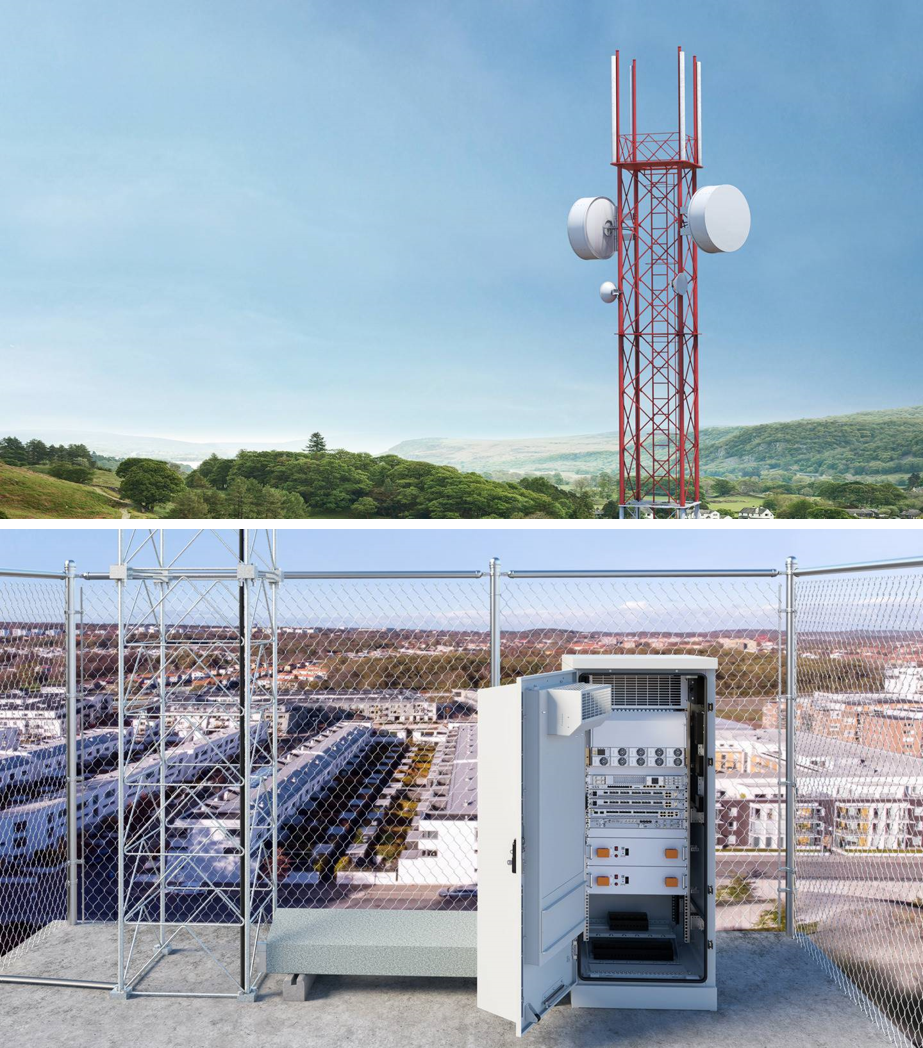
\includegraphics[width=0.42\linewidth]{figures/RBS_insfrastucture.png}
	\caption[RBS infrastructure]{RBS infrastructure. All rights belong to Ericsson}
	\label{fig:rbs_infrastucture}
\end{figure}

A \ac{rbs} is the element of telecommunication networks that receives and broadcasts electromagnetic waves to the environment in a determined area and is therefore one of the essential pieces to enable mobile communication. 

Mobile networks are geographically distributed in units called \emph{antenna site} consisting of multiple cells which comprise more than one cell --usually three--. Depending on its technology, it will vary its components and the architecture in which they are connected, as shown in Figure \ref{fig:rans}. Nonetheless, the main principles stand. 

\begin{figure}[H]
	\centering
	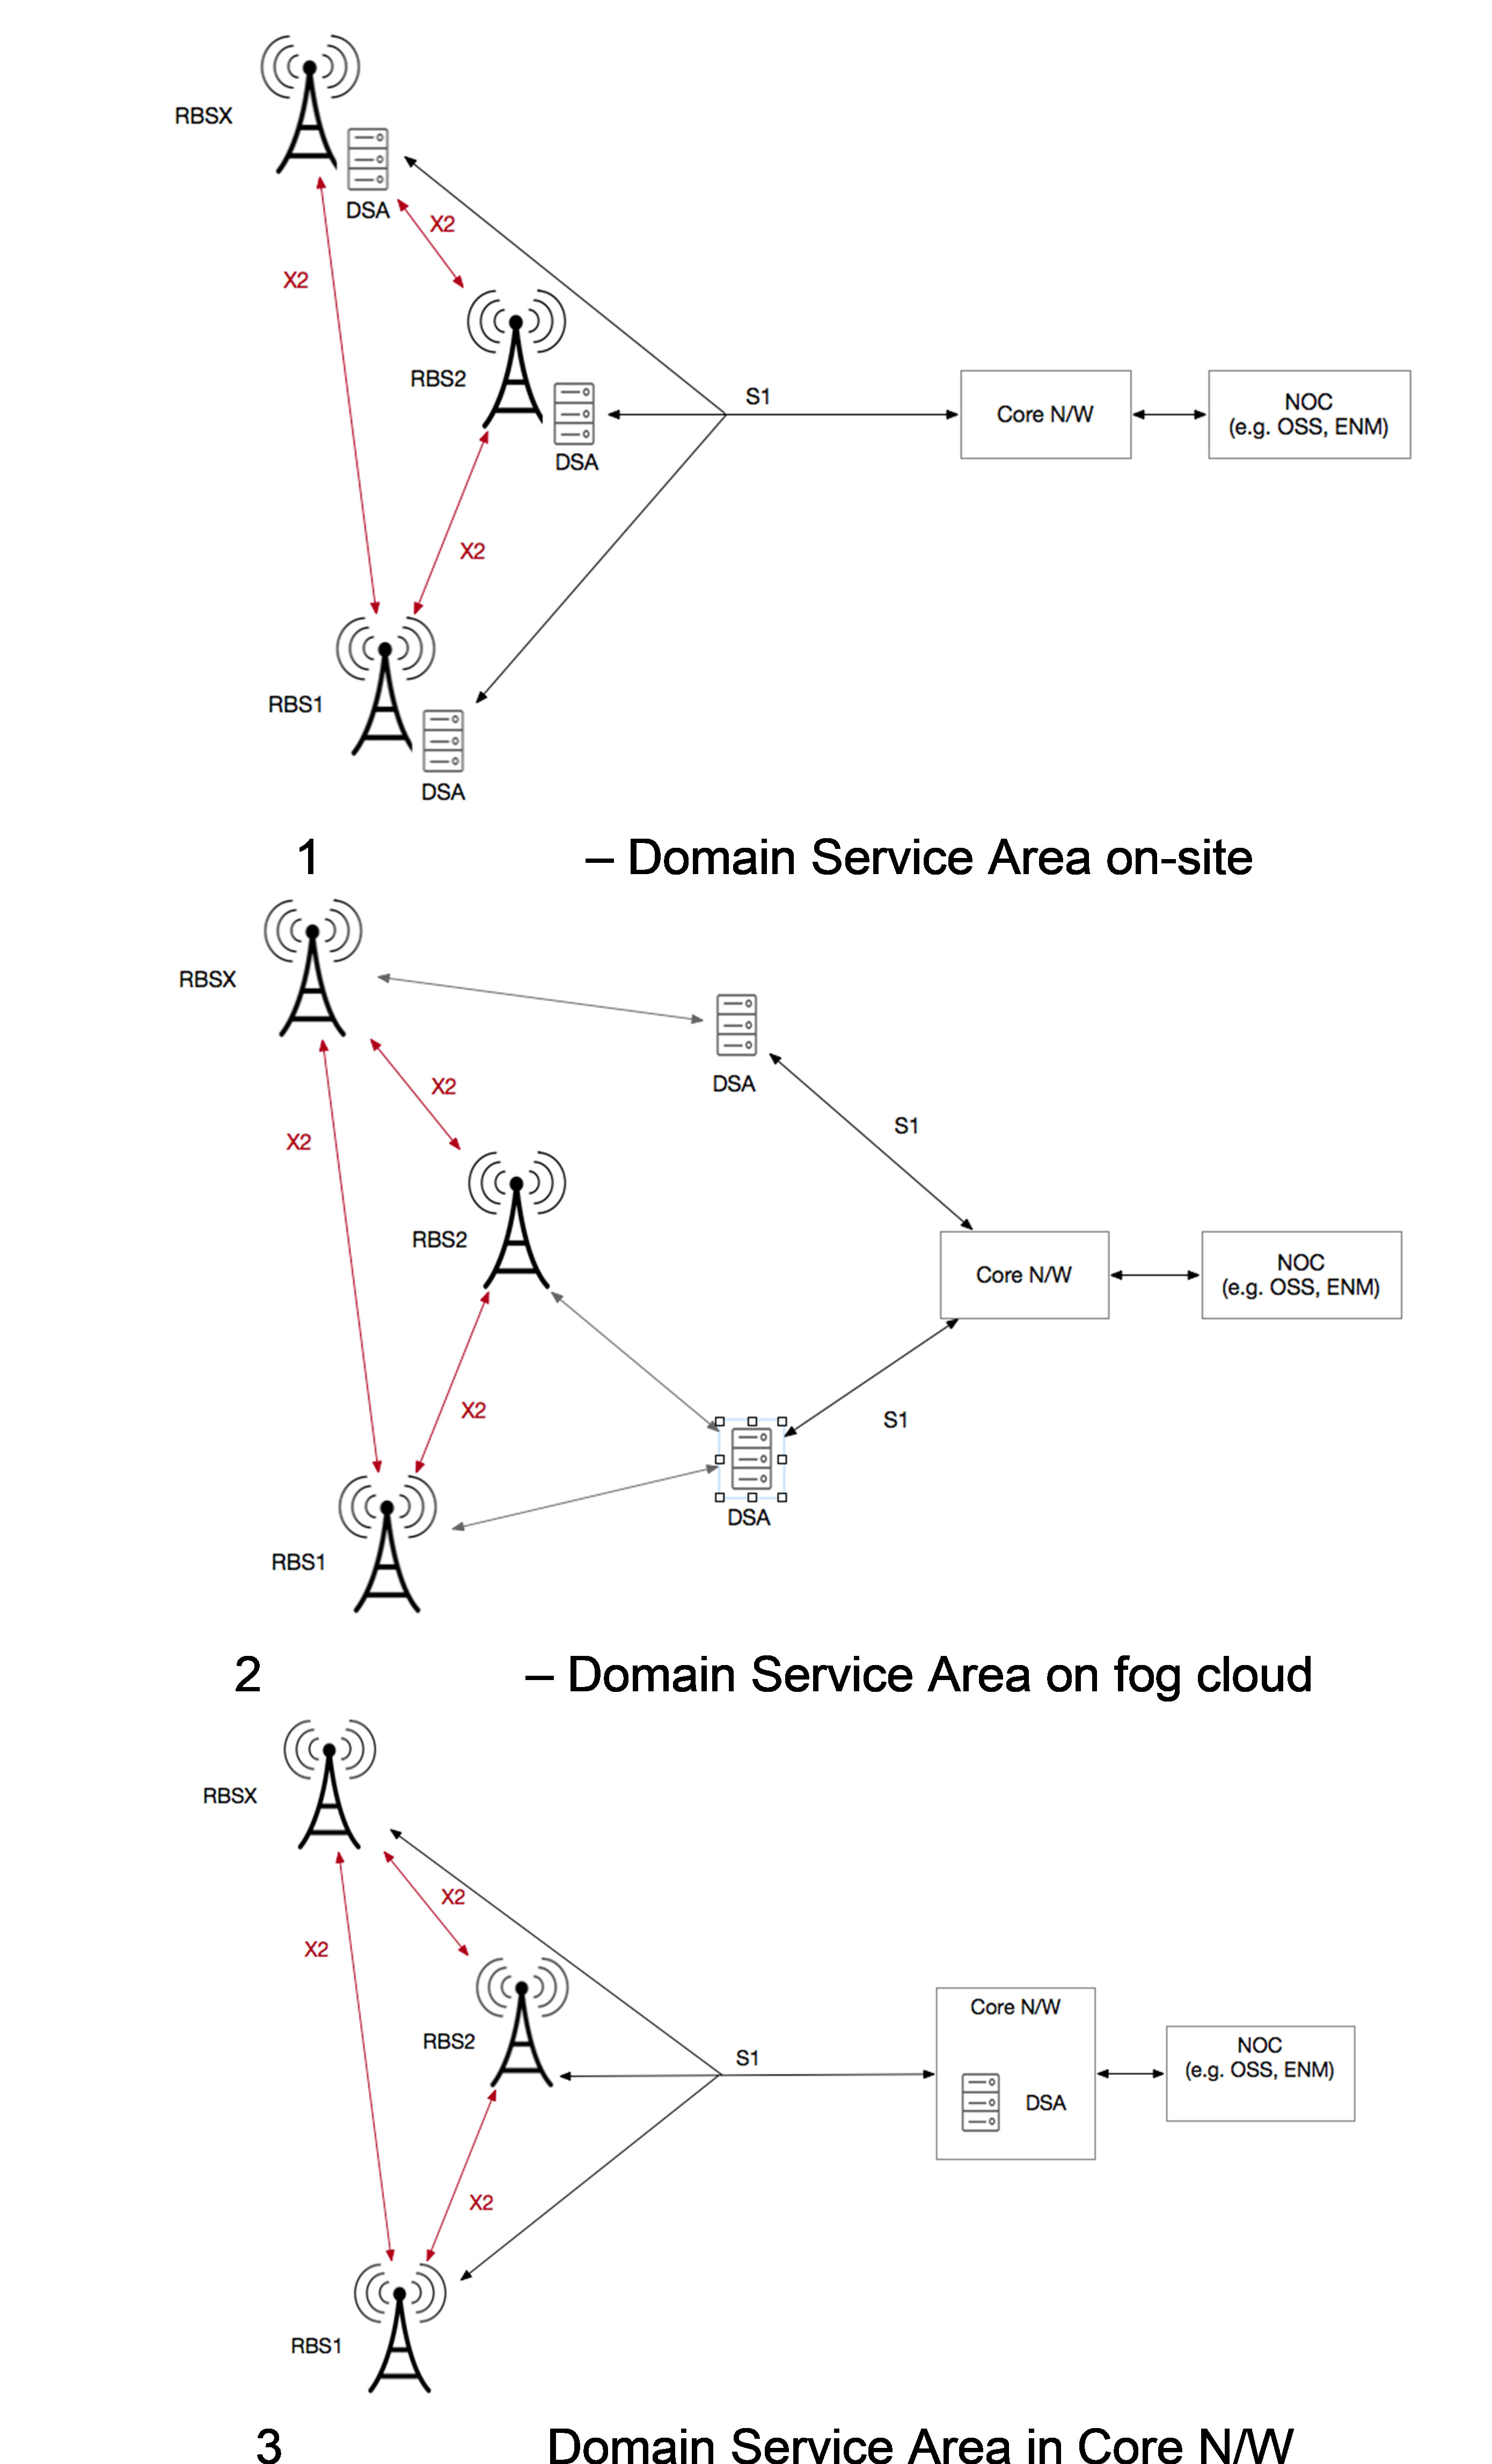
\includegraphics[height=0.9\linewidth]{figures/RANs.png}
	\caption{Different Radio Access Networks architectures}
	\label{fig:rans}
\end{figure}

In present \acp{rbs}, in case of any hardware fault,  an alarm is triggered and sent to the fault management system (reporting system) and informed to the \ac{oss} in order to be processed and handled by the \ac{noc}. Engineers in the \ac{noc} should raise a request to send the field workforce to replace the faulty unit based on the alarm data.

The reality is that not all of the alarms affect the radio performance or cause degradation of the radio traffic, which implies that there is no urgency in sending service personnel to the \ac{rbs} site until its operational continuity is at risk. 

Setting the right time for sending field workers to the \ac{rbs} to replace hardware, which sometimes might be located in very isolated or hard to reach locations,  would positively affect the maintenance and operational costs for the \acp{mno}.

%As a Statistics and Machine Learning research, the current work does not aim to provide deep knowledge on telecommunications networks. Thus, some communications concepts will not be thoroughly developed, which does not imply any lack of statistical research rigorousness.

In this thesis, the focus will be on the statistics and machine learning research rather than on communication networks development. Thus, some communications concepts will not be thoroughly developed.

\subsection{PSU alarms and power headroom}

The \acf{psu} powers the entire \ac{rbs}. Nonetheless, usually, one station may contain several \acp{psu} for operational robustness in case of faults, as shown in Figure \ref{fig:powerinfrastucture}. This redundancy implies that when an alarm is received from a \ac{psu}, sometimes, there is no need for an immediate replacement of the faulty \ac{psu} hardware since the \ac{rbs} has still enough power available to continue its operation without blackout risk. 

\begin{figure}[H]
	\centering
	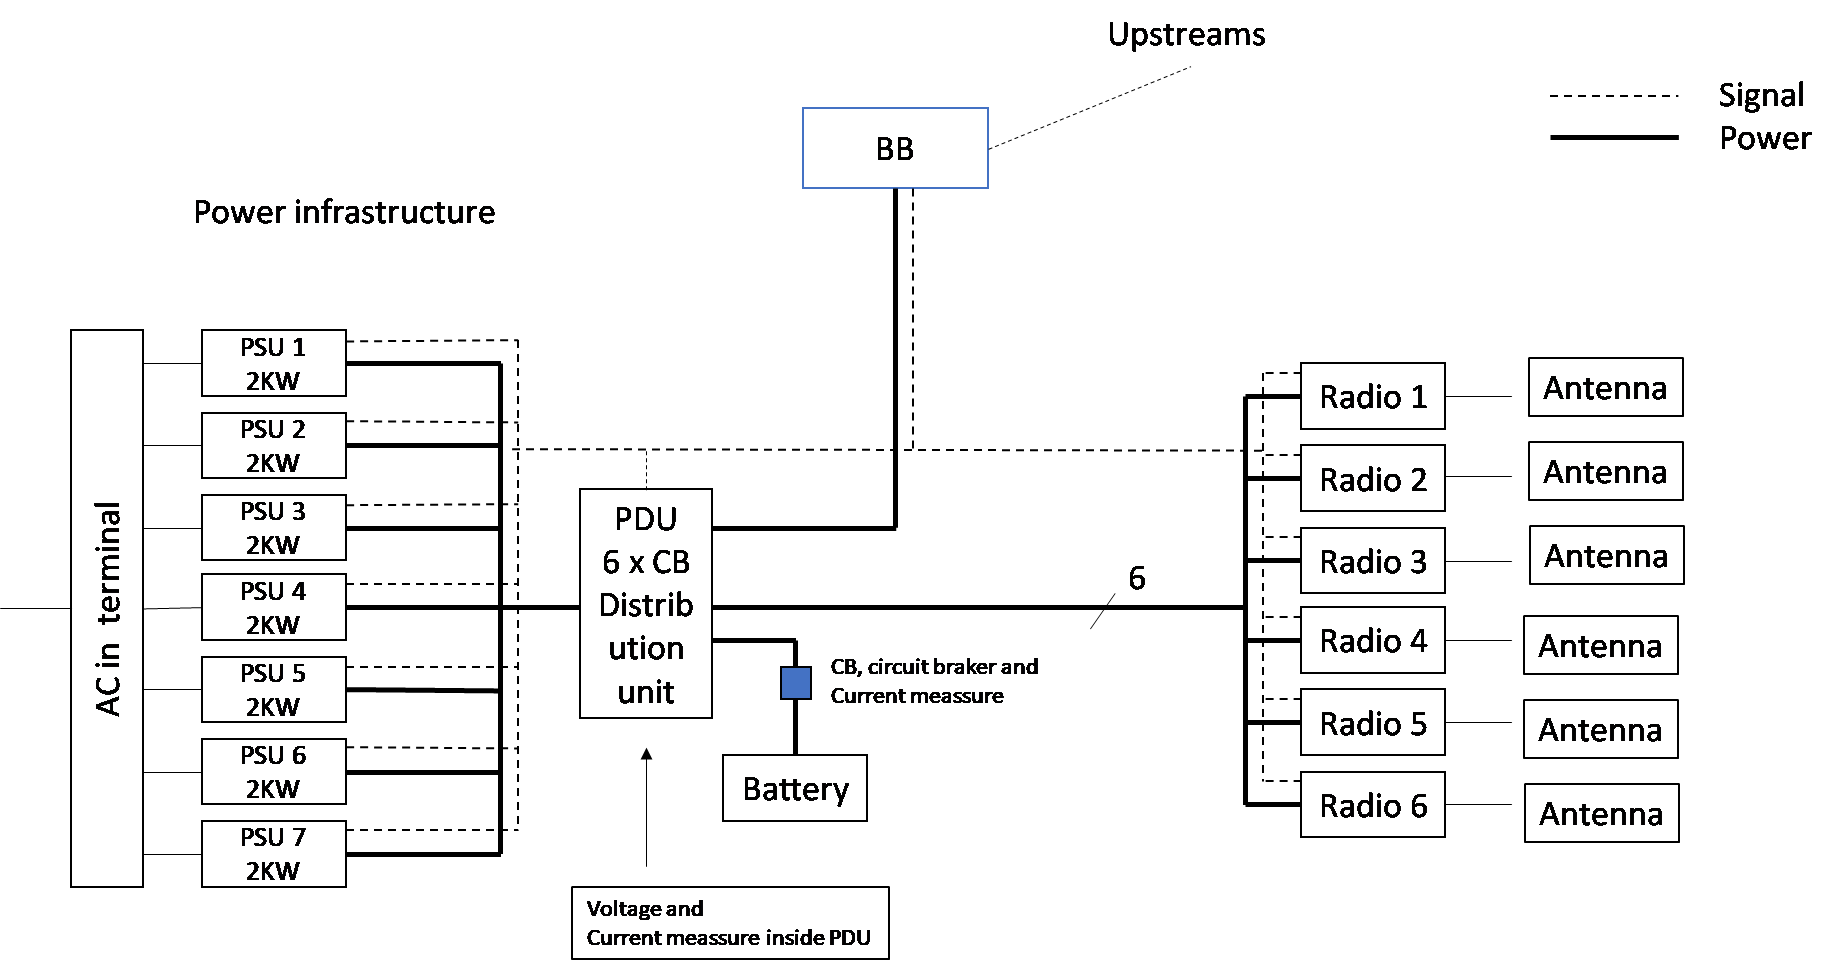
\includegraphics[width=0.95\linewidth]{figures/power_infrastucture}
	\caption[Example of a power infrastructure in an \ac{rbs}]{Example of a power infrastructure in an \ac{rbs}\protect\footnotemark}
	\label{fig:powerinfrastucture}
\end{figure}

\footnotetext{This is a general overview of the power infrastructure in an \ac{rbs}, i.e., each station may differ from others depending on how the ad-hoc solution has been designed}

Other components to note to better understand the features are the \ac{pdu} which is the unit that manages the power of the system and distributes it according to different operational scenarios. The \acp{ru} are, as its name explains, the units in which the power is converted into electromagnetic waves modulated to carry information and then uses the antennas to broadcast them into the ambient. Last but not least are the power lines, which are not a unit themselves, but interconnects the units so the \ac{rbs} itself could work as a system. The power lines are the veins that carry the energy to all the elements within the system. Nonetheless, they are not ideal, and power gets dissipated along them. The longer the lines are, the higher the losses.


Added to the power surplus given by redundant \acp{psu}, there is also the fact that not all the available power is used all the time because the radio traffic has a clear seasonal component as shown in Figure \ref{fig:connectionstwoweeks}. Thus, the \acp{ru} are not constantly transmitting at their maximum capacity.


\begin{figure}[H]
	\centering
	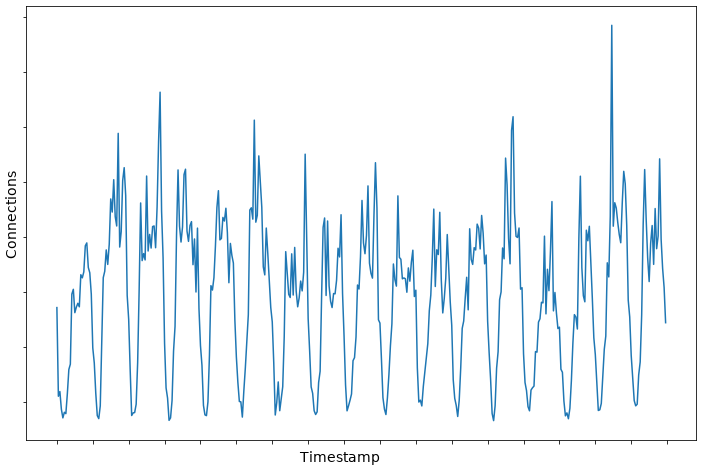
\includegraphics[width=0.8\linewidth]{figures/connections_two_weeks}
	\caption{Example of variation of a number of connections in a \ac{rbs}}
	\label{fig:connectionstwoweeks}
\end{figure}

Given this surplus in energy, the PSU \emph{power headroom}\footnote{This shall not be confused with the power headroom defined in 3GPP. We have used the same \emph{headroom} terminology so communication engineers could easily understand its main concept. But is has to be emphasised that this is related to \ac{psu} power and not to Radio power.} $P_h$ can be defined as the difference between the power consumption $P_{cons}$ and the maximum available power $P_{max}$.

\begin{equation}\label{eq:phdroom}
	P_h = P_{max} - P_{cons}
\end{equation}

Where $P_{cons}$ can be understood as \emph{the consumed power seen from the \ac{psu}} \cite{muhammad2010uplink,procedures20123gpp}, which will comprise the \acp{ru} power consumption, static power consumption, cooling system consumption, the losses in the lines, etc. For simplicity, this definition will not be developed in-depth.

In Figure \ref{fig:powerheadroom} it is shown how the amount of \acp{psu} is related to the power headroom and how a decrease in the amount of working \acp{psu} would diminish the power headroom value but still give a reasonable operational margin.   

\begin{figure}[H]
	\centering
	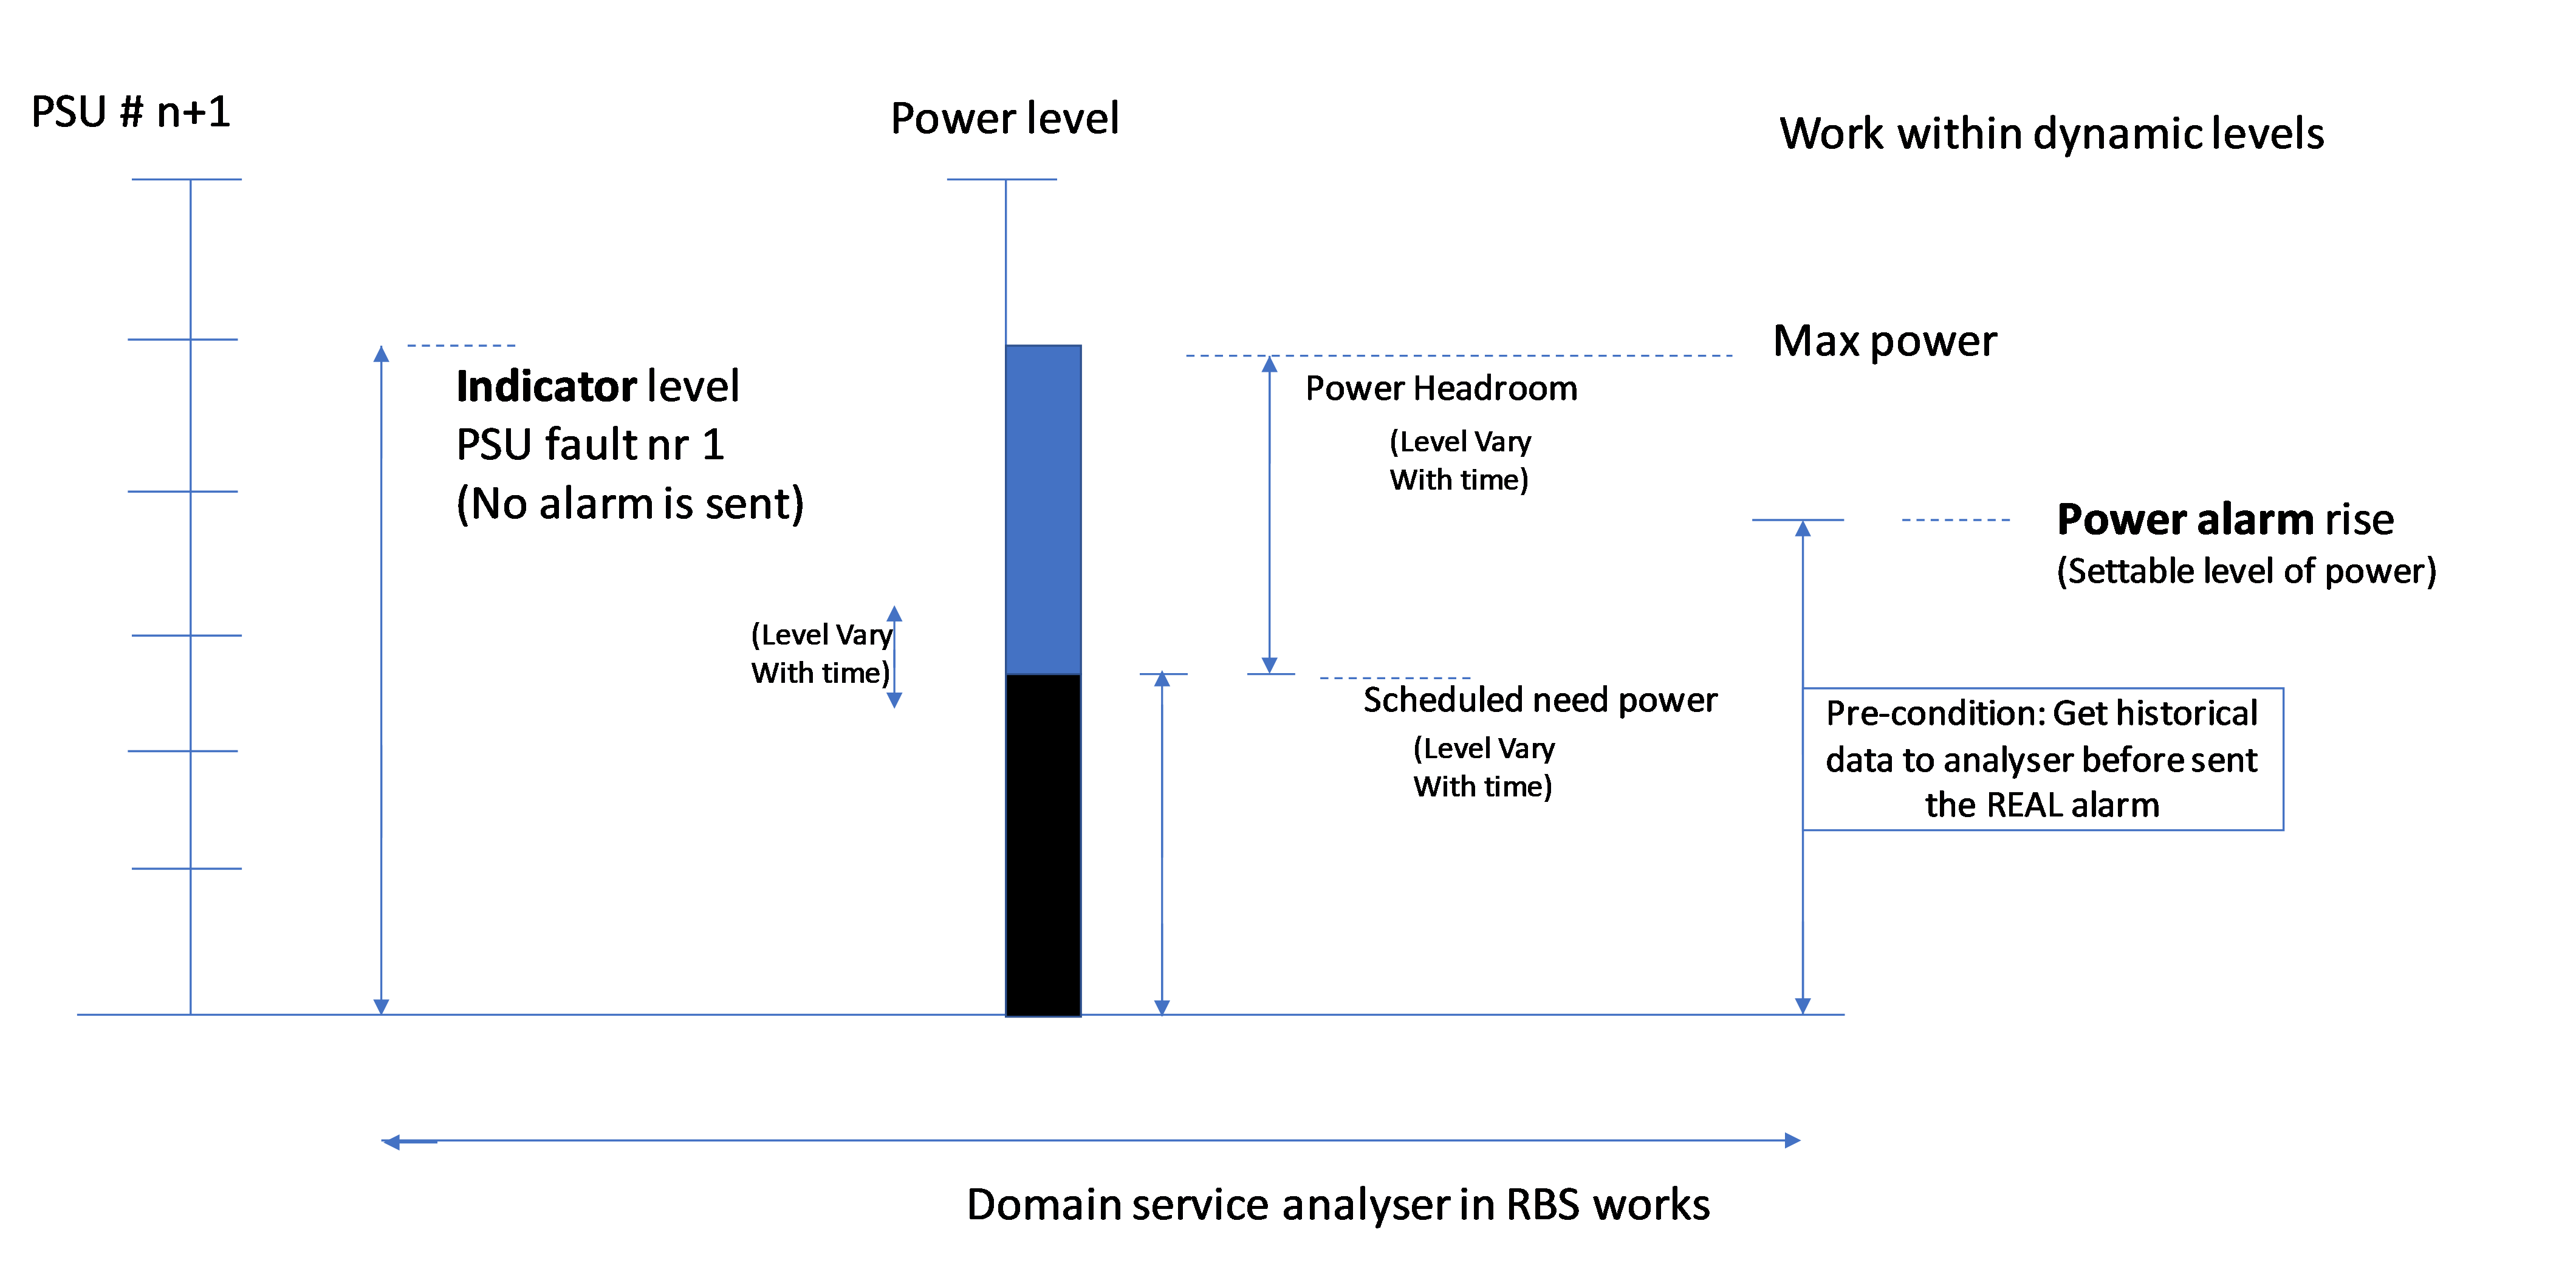
\includegraphics[width=0.95\linewidth]{figures/power_headroom}
	\caption[Power headroom]{Power headroom example}
	\label{fig:powerheadroom} 
\end{figure}



\pagebreak
\section{State-of-the-art}

The research on power consumption in \acp{rbs} is not a new topic in the communication community and it can be seen from two different research perspectives. The first stands from a modelling point of view. It can have a top-to-down approach \cite{power_modeling}, i.e., focusing on the consumption first, and based on them, describe the system. Alternatively, there is a bottom-up perspective, in which the overall power consumption of the system is described by the consumption of each independent building block depending on their different operational modes \cite{power_detailed}\footnote{ This study considers: power amplifier, analogue frontend, digital baseband, digital control and power system}. Both have in common that they are descriptive in nature and have constrained their data to pure hardware technologies and their power characteristics. Their primary purpose has been modelling and simulation of power consumption in communication networks.


The second perspective uses more data than just hardware descriptions. As a consequence, traffic metrics have been shown to be a fundamental covariate to explain power consumption fluctuations in \acp{rbs} \cite{powerregression}. Furthermore, STL decomposition has been applied to model the traffic load in \acp{rbs}. Then, Holt-Winter's technique \cite{winters1960forecasting} has been used to forecast its values, so the power management can adopt power-saving strategies when it is not needed to broadcast at maximum power capacity \cite{piunti40traffic}.

When it comes to power consumption forecast in domains other than telecommunication, the field has also been fruitful. Sensor network's power consumption using Markov chains \cite{achir2004power}, power consumption in data centres using LASSO, elastic-net, \ac{rf}, KNN, and \ac{mlp} \cite{deepika2020power}, coal-mining power consumption forecast using pure statistics \cite{antonenkov2017mathematic} or laser-melting processes using linear regression \cite{lv2020novel}, to mention some.  

Furthermore, forecast household power demand is a very fertile domain on its own. Linear regression, decision trees, \ac{rf}, \ac{svr} and \ac{mlp} have been applied to predict the demand in northern Morocco \cite{morocco} finding that \ac{mlp} performs better than the others. \ac{lstm} networks have been applied to learn household consumption and have been compared against \ac{gbt} and \ac{svr} approaches finding that the \ac{lstm} model, which they have called \emph{PowerLSTM}, outperforms the others\cite{powerlstm}. A novel \ac{eennp} method is proposed in \cite{ai2019household} and applied to power consumption in western Norway. 

The well-used Holt-Winters model has been compared against Facebook's Prophet model in long-range power loads forecast in Kuwait, reaching a $\text{MAPE}\sim2\%$ for a prediction horizon of 720 days. Their predictions robustness has been tested by injecting Gaussian noise in different intensities at a fixed (unspecified) forecasting horizon, concluding that Prophet can perform robust power demand predictions while obtaining $R^2=0.96$ at a noise intensity of $80\%$ \cite{almazrouee2020long}. In the same direction, it has been shown that Prophet performs better than ARIMA models for a long-range of 30 days on power demand prediction using external environmental regressors in an airport in Belgium \cite{chadalavada2020electricity}. In both studies, Prophet's weekly seasonal component is used to recommend the most suitable day of the week to perform maintenance related to power consumption.  

Furthermore, in \cite{jiang2021clothing}, the potential of Prophet for long-range predictions has been shown by extending it to work together with a \ac{gru} as an attention layer plus a \ac{critic} node to weigh both predictions optimally. For a prediction horizon of $\sim6$ months, the proposed architecture show a $\text{MAE}=8.5$ against $10.1$ and $20.1$ from Prophet on its own and ARIMA, respectively.  

%Thus, the robustness of the predictions made by Prophet models for long-range time horizons makes it an interesting alternative to be applied in the telecom domain. Additionally, it has shown to perform better than standard methods in other fields, which are also highly related to human behaviours. No publication has been found doing so during the research.

Thus, the robustness of the predictions made by Prophet models for long-range time horizons in addition to that it has shown to perform better than standard methods in other fields, which are also highly related to human behaviours, makes it an interesting alternative to be applied in the telecom domain. No publication has been found doing so during the research.



\pagebreak
\section{Aim}
\label{sec:aim}

The following work aim to develop a statistical or machine learning method that reports an alarm if, and only if, the power headroom in a \ac{rbs} will reach unsafe operational levels based on installed power capacity and power consumption forecasts. 

Based on state-of-the-art findings, exploring Prophet's capabilities to also endow of long-range robustness the proposed solution.


\section{Research questions}
\label{sec:research-questions}

\begin{enumerate}
	\item What is the best way to handle real-world telecommunication and power time series to provide useful structures to mine and learn from them?
	\item What are suitable forecast techniques to predict power utilisation in an \ac{rbs}?
	\item Given the power forecast, what are suitable criteria to raise alarms, if and only if, the \ac{rbs} operational continuity is at risk?
\end{enumerate}

\section{Delimitations}
\label{sec:delimitations}


Even though one of the overall goals of the work has been reducing operational costs for \acp{mno}, this has been done without considering the logistics under maintenance, or stock constraints of hardware replacement stock or even \ac{rbs} geographical location. Therefore, the only factor of operational costs this work tries to optimise is \emph{when} a hardware replacement alarm is raised.




\chapter{Data analysis}
\label{cha:data_analysis}

\section{Data acknowledgements}

Due to data usage legal restrictions and Ericsson's customers' privacy, internal identifiers used by the company's operations and dates in all timestamps have been anonymised in the thesis available for the public domain. Moreover, the data structures and sensitive data values have not been presented.

\section{Data description}
\label{sec:data_description}

The available data is in the form of time series indexed by an \ac{rbs} unique identifier and the time stamp corresponding to sample time. The data is sparse and in different files depending on the domains from where the features have been measured, i.e., the power supply, power distribution, radio traffic, cabinet climate, etc. A brief explanation of the information provided by the time series and some random samples from the database are shown in the following subsections. It should be noted that configuration data for base stations is included. This data shows hardware equipment and their settings, for example, the number of \acp{psu}. 

\subsection{Power supply}
\label{subsec:data_description:power_supply}

\subsubsection*{Power supply interruptions from the Power Grid distribution}

This measurement shows how stable the electric power supply from the AC distribution is, i.e., it is a time counter in which the energy supply has been interrupted from the public power distribution. 
As a consequence, \ac{rbs} utilise power from other sources such as batteries.

\subsubsection*{\ac{psu} utilisation statistics}

\ac{psu} utilisation refers to the percentage of \ac{psu}'s power capacity being consumed by the loads over a determined time. In the available data for this project, this is described by the average, minimum, maximum and standard deviation of these measures over different time durations.

These statistics are, in fact, the most crucial feature in the present work. It can be understood as the complement of the power headroom in per cent. In order to obtain the power values in terms of Watt, the installed power capacity needs to be known. 

As there are no direct power headroom measurements, the \ac{psu} utilisation has been chosen as the target variable, and then the power headroom will be derived from this quantity. In the Figure \ref{fig:feats_avgpsu}, the average of a \ac{psu} utilisation is shown as an example. 

\begin{figure}[hptb]
	\centering
	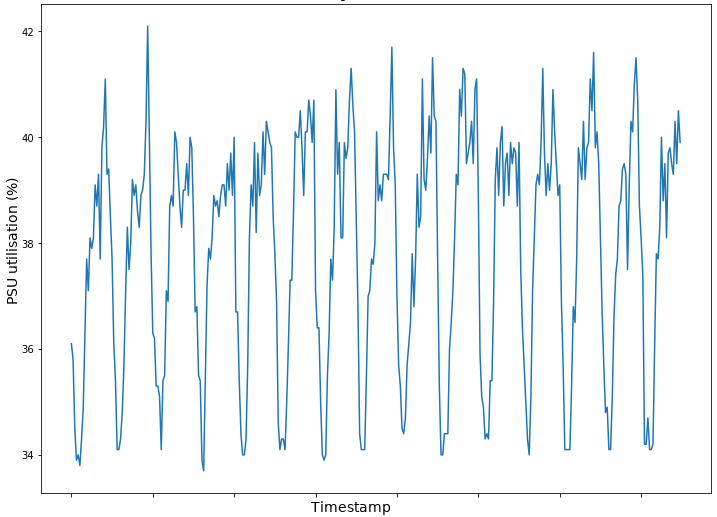
\includegraphics[width=0.65\textwidth]{avg_psu_utilization}
	\caption{Average PSU utilisation example}
	\label{fig:feats_avgpsu}
\end{figure}


\subsection{Radio energy}

\subsubsection*{Radio units voltage statistics}

The \acp{ru} are fed with energy by the \ac{pdu}. Nonetheless, this is not constant and might change over time. The minimum, maximum, average and standard deviation statistics show how these fluctuations have been over a determined time. Figure \ref{fig:feats_std_ru_voltage} shows the standard deviation of the voltage perceived by the \acp{ru}. 

\begin{figure}[hptb]
	\centering
	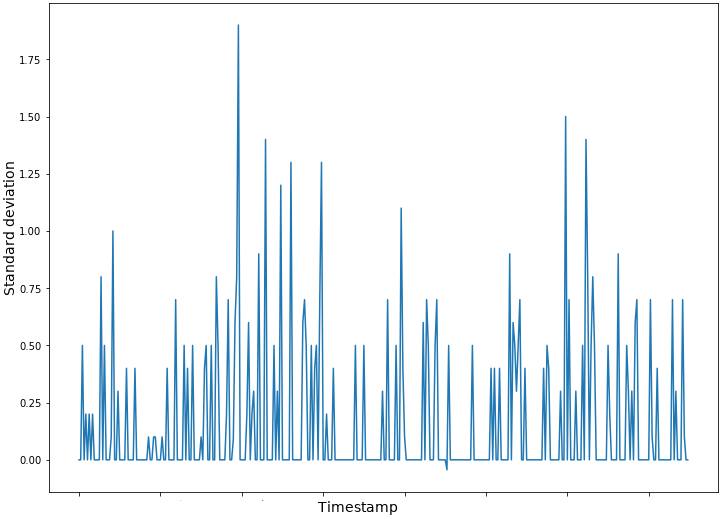
\includegraphics[width=0.65\textwidth]{std_ru_voltage}
	\caption{Standard deviation of \ac{ru} voltage example}
	\label{fig:feats_std_ru_voltage}
\end{figure}

\subsubsection*{Radio units power consumption statistics}

Supplied energy and power consumption are not the same. Whereas the former refers to the available energy to be used, the consumed power refers to the actual power used for broadcasting purposes. The minimum, maximum, average and standard deviation statistics have been measured and reported over a determined time. Figure \ref{fig:feats_avg_ru_power_consumption} presents the average of the consumed power by the \ac{ru} as an example.

\begin{figure}[hptb]
	\centering
	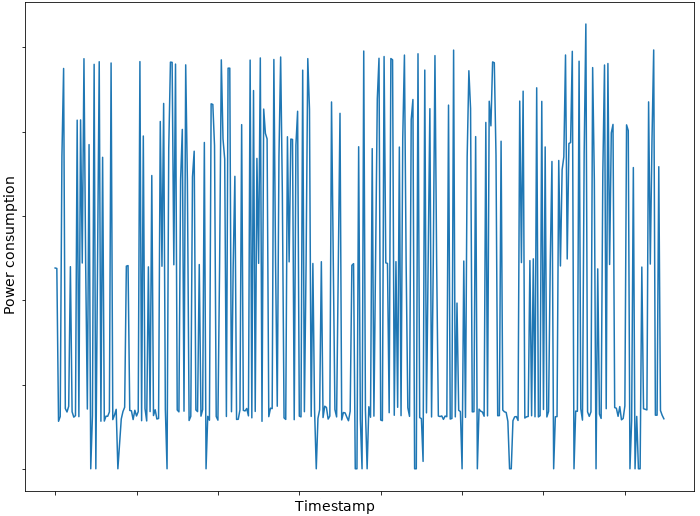
\includegraphics[width=0.65\textwidth]{avg_ru_power_consumption}
	\caption{Average \ac{ru} power consumption example}
	\label{fig:feats_avg_ru_power_consumption}
\end{figure}

\subsection{Power distribution}

As shown in Figure \ref{fig:powerinfrastucture}, the \acp{ru} are not fed directly by the \acp{psu} but by the \ac{pdu} which manages the different power sources of the \ac{rbs}. The measurements in the \ac{pdu} do not need to be the same as the voltage and power measurements in the \acp{ru} because the power lines that connect them could be up to 60 metres long, which might introduce some losses to the system.

Like other features, these are sampled and presented as their minimum, maximum, average and standard deviation over a determined time. Figure \ref{fig:feats_avg_pdu_voltage} shows the average of the \ac{pdu}'s output voltage as example.

\begin{figure}[hptb]
	\centering
	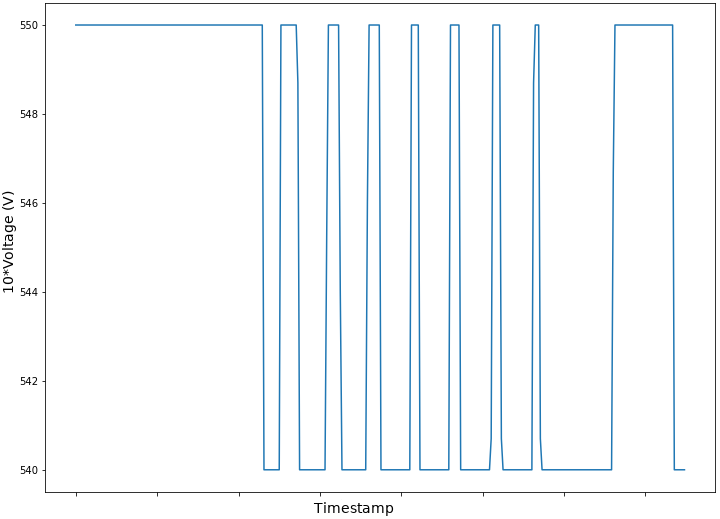
\includegraphics[width=0.65\textwidth]{avg_pdu_voltage}
	\caption{Average \ac{pdu} voltage example}
	\label{fig:feats_avg_pdu_voltage}
\end{figure}


\subsection{Radio traffic}

In the data measured from radio traffic, it is possible to observe the highly seasonal characteristics of users behaviour influenced by the day-night cycle. Examples of data are shown in Figures \ref{fig:feats_connections}. \ref{fig:feats_data_blocks}, and \ref{fig:feats_active_users}. 

\subsubsection*{Number of connections}

This measurement corresponds to the number of established connections to the radio traffic.

\begin{figure}[H]
	\centering
	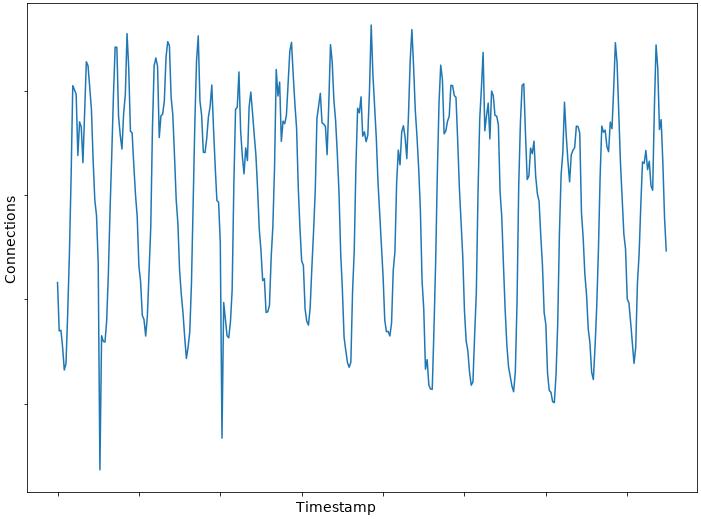
\includegraphics[width=0.65\linewidth]{connections.png}
	\caption{Connections requests signal example}
	\label{fig:feats_connections}
\end{figure}

\subsubsection*{Data blocks}

This signal corresponds to the number of resource blocks connected to the traffic load in the uplink and downlink.

\begin{figure}[H]
	\centering
	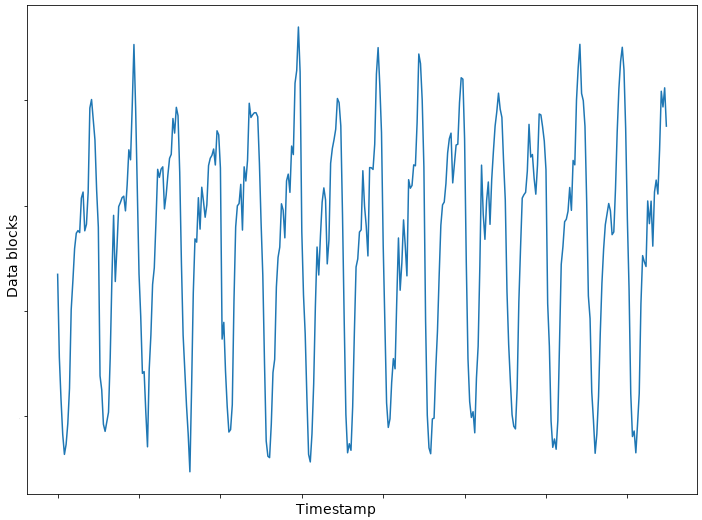
\includegraphics[width=0.65\linewidth]{data_blocks.png}
	\caption{Data blocks signal example}
	\label{fig:feats_data_blocks}
\end{figure}

\pagebreak
\subsubsection*{Active Users}

This feature shows the number of active users connected to the radio traffic load in the uplink and downlink.

\begin{figure}[H]
	\centering
	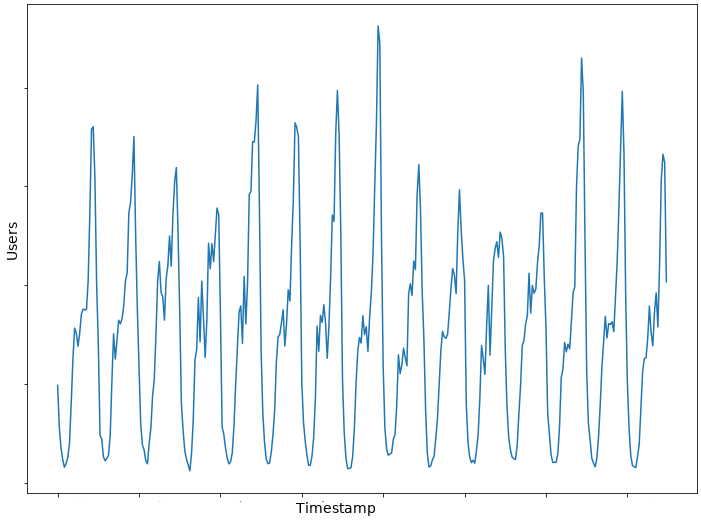
\includegraphics[width=0.65\linewidth]{active_users.png}
	\caption{Active users signal example}
	\label{fig:feats_active_users}
\end{figure}


\subsection{Climate}

\subsubsection*{Average cabinet temperature}

In electronic components, high temperature is highly correlated with power dissipation; therefore, its increments in the hardware units will also increase the temperature within the cabinet. An example of average cabinet temperature time series is shown in Figure \ref{fig:feats_cabinet_temp}. 

\begin{figure}[H]
	\centering
	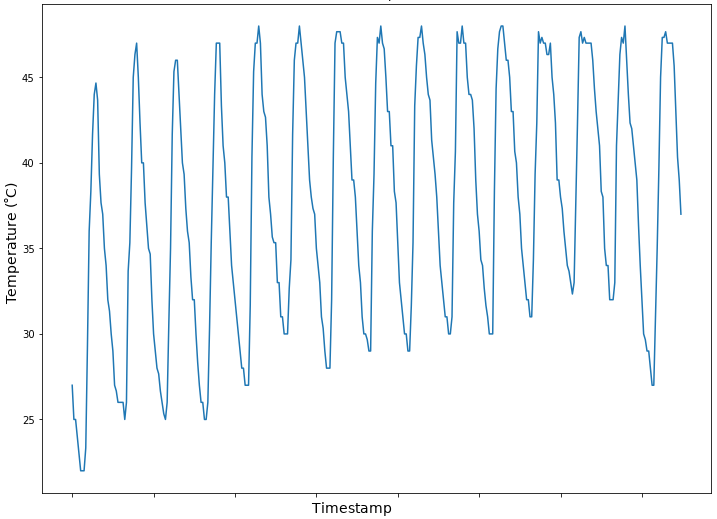
\includegraphics[width=0.65\linewidth]{cabinet_temp.png}
	\caption{Cabinet temperature signal example}
	\label{fig:feats_cabinet_temp}
\end{figure}

\pagebreak
\subsubsection*{Internal and external fan speed}

The cabinet is designed to keep the hardware safe. When the cabinet temperature is considered \emph{high}, the fans, one internal and the other external, will be managed to cool down the hardware units. Therefore, the higher the temperature, the faster the fans will run. The reported values correspond to percentages of possible speed values, i.e.,  a zero value represents a steady fan, whereas a 100 means maximum velocity. Internal and external fan speed signals are shown in Figure \ref{fig:feats_int_fan} and \ref{fig:feats_ext_fan}.

\begin{figure}[hptb]
	\begin{subfigure}{.47\textwidth}
		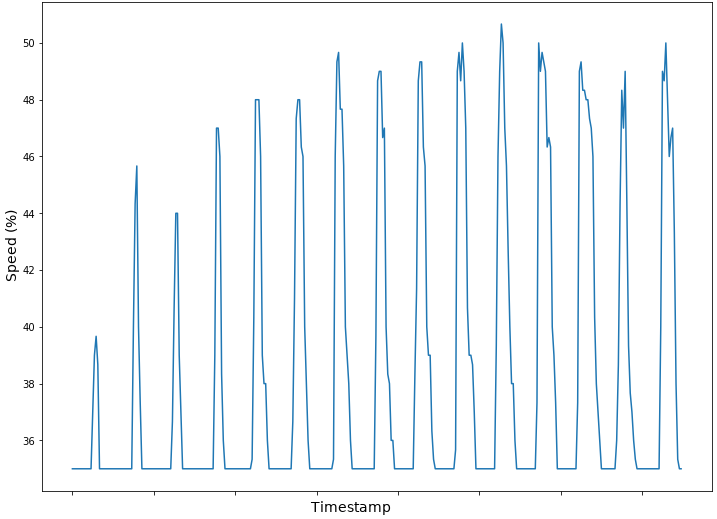
\includegraphics[width=\textwidth]{internal_fan}
		\caption{Internal fan speed}
		\label{fig:feats_int_fan}
	\end{subfigure}%
	\hfill
	\begin{subfigure}{.47\textwidth}
		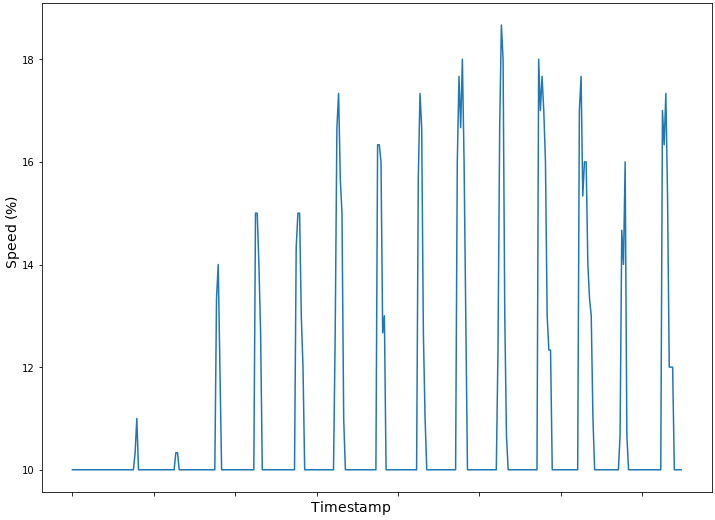
\includegraphics[width=\textwidth]{external_fan}
		\caption{External fan speed}
		\label{fig:feats_ext_fan}
	\end{subfigure}
	\caption{Internal and external fan speed signals examples}
\end{figure}



\chapter{Theory}
\label{cha:theory}

\section{Data imputation and database construction}


In general, when measuring any variable and collecting data there is always a risk of missing some data samples. Examples can be people not answering some questions in surveys or incomplete medical records, or even public entities failing to report data or choosing not to disclose it. Sampling data from sensors and reporting it via wireless communication channels is not invulnerable to this type of issues. There can be unforeseen technical issues such as a car crash damaging some units, power blackouts, or even a misconfiguration done by a negligent engineer.

Therefore, handling missing data is a problem that has been under research for a long time. Multiple Imputation \cite{imputationRubin}, Expectation-Maximization \cite{imputationEM}, Nearest Neighbours \cite{imputationNN} and hot-deck \cite{imputationHotDeck} are the most popular techniques to deal with them.

In the following sections, it is going to be exposed how it is possible to obtain approximations of the processes that produce a given time series, and how these approximations can be used to \emph{fill the gaps} of missing data through imputation processes.

%As in the previous step, and based on time constraints, it has been decided not to implement algorithms from scratch but rely on existing known packages to avoid investing in developing time. 
%
%Moritz et al. have analysed several univariate time series imputation implementations in R \cite{MoritzComparison}, which results later have been compiled in the \texttt{imputeTS} R package \cite{imputeTS}. Therefore, it is reasonable to rely on their work and use their results to decide which imputing strategy should be taken. 
%Thus, for the current work, the \texttt{imputeTS} package will estimate a structural time series model from the data and then perform the Kalman smoothing to fill the gaps. 
%
%It should be noted that before performing the Kalman smoothing, it is needed to have a state representation of the model, for which \texttt{imputeTS} supports Auto-ARIMA state-space estimation and structural time series model fitted by maximum likelihood. In addition, it should be mentioned that the development has been mainly done in python. Nonetheless, for this phase, an R package will be called from Python using the \texttt{rpy2} module as an interface to bounce between both languages.


\subsection{Notation}

In the following sections, mathematical notations will be used from time series analysis. In order to stand on common ground,  notations are defined and their meaning explained.

\subsubsection*{Backshift operator}

The \emph{backshift} ($B$) or \emph{lag} ($L$) operators refer to the same operation and both can be found in the literature with no different meaning. In the current work it will , let us define \ref{eq:backshift_def}

\begin{definition}[Backshift operator]
	\label{eq:backshift_def}
	Let $B$ denote a backshift or a lag operation in a given series $\{Y_t\} = \{Y_1, Y_2, \ldots, Y_n\}$ such that $ t,n \in \mathbb{N}, t \leq n$ as 
	
	\begin{equation}
		B Y_t = Y_{t-1}, \quad t>1
	\end{equation}
\end{definition}

\begin{property}[Inverse Backshift]
	\label{eq:inv_bs_op}
	The inverse operation of a lag it is a forward step, thus
	\begin{equation}
		B^{-1}Y_t = Y_{t+1}
	\end{equation}
\end{property}

\begin{property}
	The backshift exponentiation introduced in Property \ref{eq:inv_bs_op} can be generalised to denote back/forward shifts in multiple steps as	
	\begin{equation}
		B^{k}Y_t = Y_{t-k}
	\end{equation}
\end{property}


\begin{property}[Backshift algebra]
	$B$ is a linear operator. Therefore the following is always true.
	
	\begin{align}
		B(aX_t + bY_t + c) &= aBX_t + bBY_t + c \\
		B^jB^k Y_t &= B^{j+k}Y_t
	\end{align}
\end{property}

\begin{property}[Backshift polynomials]
	
	The backshift operations can be treated as polynomials to explain more complex expressions.
	
	Let $\{Y_t\} = \{Y_1, Y_2, \ldots, Y_n\}$ be a random process and $\bm{\alpha} = (\alpha_1, \alpha_2, \ldots, \alpha_n)$ such that.

	
	\begin{equation}
		\label{eq:bs_poly}
\begin{split}
		\alpha_{t-1} Y_{t-1} + \alpha_{t-2} Y_{t-2} + \ldots + \alpha_{t-k} Y_{t-k} &=\alpha_{t-1} BY_{t} + \alpha_{t-2} B^2Y_{t} + \ldots + \alpha_{t-k} B^kY_{t} \\
		&=(\alpha_{t-1}B + \alpha_{t-2}B^2 + \ldots + \alpha_{t-k}B^k) \{Y_{t}\}\\
		&=\alpha(B)\{Y_{t}\}
\end{split}
	\end{equation}
	 
The reduction in (\ref{eq:bs_poly}) shows the power of the backshift operator, allowing to reduce such large expression into a short and elegant one. Nonetheless, a common flaw in this notation that could create confusion is that it is not needed to specify the polynomial order ($k$ in the example). It can be assumed that whenever the order is not specified is then a general expression for any $k$-th order polynomial. Nonetheless, whenever its specification is needed, such as to specify an AR or MA model order, a subscript to the notation can be added: $\alpha_k(B)$ in this example.    
	 
\end{property}

\subsubsection*{Difference operator}

It is also used the (backward) difference operator used in finite difference calculus to simplify long differences expressions. 

\begin{definition}[Difference operator]
	Let $\nabla$ denote the difference operator in a given series $\{Y_t\} = \{Y_1, Y_2, \ldots, Y_n\}$ such that $ t,n \in \mathbb{N}, t \leq n$ as 
	
	\begin{equation}
		\nabla Y_t = Y_t - Y_{t-1}, \quad t>1
	\end{equation}
\end{definition}

\begin{property}[Difference and backshift operators relation]
	As an operation between lagged values, it is possible to define $\nabla$ in terms of $B$
	
	\begin{align}
		\begin{split}
			\nabla Y_t 	&= Y_t - Y_{t-1} \\
			\nabla Y_t	&= Y_t - BY_t \\
			\nabla Y_t	&= (1-B)Y_t
		\end{split}
	\end{align}
\end{property}

\begin{property}[High order differences]
	Let us obtain the second-order difference as	
	
	\begin{align}
		\label{eq:2nd_nabla}
		\begin{split}
			\nabla (\nabla Y_t)	&= \nabla Y_t - \nabla Y_{t-1} \\
			\nabla^2 Y_t		&= \nabla Y_t - \nabla B Y_{t} \\
			\nabla^2 Y_t		&= (1-B) \nabla Y_{t} \\
			\nabla^2 Y_t		&= (1-B)(1-B) Y_{t} \\
			\nabla^2 Y_t		&= (1-B)^2 Y_{t} \\
		\end{split}
	\end{align}

	It can be shown that the development in (\ref{eq:2nd_nabla}) can be extended to the $d$-th order difference operator having that
	
	\begin{equation}
		\nabla^d Y_t = (1-B)^d Y_t
	\end{equation} 
\end{property}



\subsection{ARIMA models}

It is defined that a time series $\{X_t\}$ can be modelled by an \emph{integrated autoregressive moving average} (ARIMA) model if there exist a $d$-th difference $\{Y_t\} = \nabla^d \{X_t\}$ that can be modelled as an ARMA model \cite{brockwell2016introduction}. 

Expanding the definition 

\begin{align}\label{eq1}
	\begin{split}
		\{Y_t\} &= \nabla^d \{X_t\}, \quad d>0 \\
		&= (1-B)\nabla^{d-1}\{X_t\} \\
		& \quad\quad \vdots \\
		&= (1-B)^{d-1}\nabla\{X_t\} \\
		&= (1-B)^d \{X_t\} 
	\end{split}
\end{align}

Therefore, $(1-B)^d \{X_t\}$ will be explained by an $\text{ARMA}(p,q)$ model if the following recursive equation has a causal and stationary solution:

\begin{equation*}
	Y_t - \phi_1Y_{t-1} - \cdots - \phi_pY_{t-p} = Z_t + \theta_1Z_{t-1} + \cdots + \theta_qZ_{t-q}
\end{equation*}

Where $\{Z_t\}$ is an uncorrelated noise sequence and $\phi_i$ and $\theta_j$ are the autoregressive and moving-average weights, respectively. Written using backshift operator:

\begin{align}\label{eq2}
	\phi(B)\{Y_t\} &= \theta(B) Z_t \quad,\quad Z_t \sim \mathcal{N}(0,\sigma^2)
\end{align}

Replacing \ref{eq1} in \ref{eq2} the $\text{ARIMA}(p,d,q)$ process that explains $\{X_t\}$ can be defined as:

\begin{align}\label{eq:arima}
	\phi(B)(1-B)^d \{X_t\} &= \theta(B) Z_t
\end{align}

Where $p$ is the $p$-order of the AR($p$) process, $q$ the $q$-order of the MA($q$) process and $d$ the successive differencing steps until obtaining a stationary ARMA($p,q$) process.

\subsection{SARIMA}

It is said that a time series has a seasonality of period $s$ if $Y_t = Y_{t-s}$. Written using the backshift operator this is $Y_t = B^sY_t$.

Using the same logical development than for ARIMA derivation, it can be said that $\{Y_t\}$ follows a Seasonal ARIMA (SARIMA) process with period $s$ \cite{brockwell2016introduction} :

\begin{equation*}
	\{Y_t\} \sim \text{ARIMA}(p,d,q)(P,D,Q)_s
\end{equation*}

If and only if (\ref{eq3}) is a causal ARMA process defined by (\ref{eq4}).

\begin{equation}\label{eq3}
	\{X_t\} = (1-B)^d (1-B^s)^D \{Y_t\}
\end{equation}

\begin{equation}\label{eq4}
	\phi(B)\Phi(B^s)X_t = \theta(B)\Theta(B^s)Z_t , \quad\{Z_t\} \sim \mathcal{N}(0,\sigma^2)
\end{equation}

Therefore, replacing (\ref{eq3}) in (\ref{eq4}), the SARIMA definition can be rewritten as

\begin{equation*}\label{eq5}
	\phi(B)\Phi(B^s)(1-B)^d (1-B^s)^D \{Y_t\} = \theta(B)\Theta(B^s)Z_t , \quad\{Z_t\} \sim \mathcal{N}(0,\sigma^2)
\end{equation*}

Most of the literature obviate a constant $c$ as part of the model since it does not add more insight about the concepts around these derivations. Nonetheless, as it will be seen in the following section it is considered as part of the auto-ARIMA estimation, therefore, the final ARIMA definition in this work is given by:

\begin{equation}\label{eq:sarima}
	\phi(B)\Phi(B^s)(1-B)^d (1-B^s)^D \{Y_t\} = c + \theta(B)\Theta(B^s)Z_t , \quad\{Z_t\} \sim \mathcal{N}(0,\sigma^2)
\end{equation}

Where $p, d$ and $q$ refer to the AR, integral and MA parameters of the ARIMA model, respectively. $P, D$ and $Q$ are the AR, integral and MA parameters of the seasonal construction for the period $s$.






\subsection{State space representation}

A state-space representation of a time series is suitable for cases in which the underlying nature of a process is hidden and cannot be determined. Nonetheless,  indirect observations can be measured.

Thus, state-space representations are given by two equations. The \emph{observation equation} (\ref{eq:obs}) relates $w$-dimensional observable measures as a linear function of the $v$-dimensional noisy hidden state, and the \emph{state equation} (\ref{eq:state}) determines how the hidden state will transition from time $t$ to $t+1$.

\begin{align}
	\bm{Y}_t		&=	G\bm{X}_t + \bm{W}_t  \label{eq:obs} \\
	\bm{X}_{t+1}	&=	F\bm{X}_t + \bm{V}_t \label{eq:state} 
\end{align}

Where $F$ is a $v \times v$ matrix, $G$ a $w \times v$ matrix, $\{\bm{W}_t\} \sim \mathcal{N}(0,R)$, $\{\bm{V}_t\} \sim \mathcal{N}(0,Q)$ and $E(\bm{V}_s\bm{W}^T_t) = 0$ for all $t, s$.

\subsection{Structural models}

The classical structural models are defined in terms of trend $(m)$, seasonal $(s)$ and noise $(\varepsilon)$ components (\ref{eq:struct}). Although useful for some applications, they can be too deterministic for some others.

\begin{equation}\label{eq:struct}
	X_t = m_t + s_t + \varepsilon_t
\end{equation}

State-space representations allow bringing more flexibility to these components. Therefore, it is natural to extend these concepts to a state-space domain. 

\subsubsection{Local level model}

To show how the model is built up, it will be derived by adding component by component from the most straightforward model: the random walk. Let $\{Y_t\}$ be the observable variable from a state-space (\ref{eq:loclvl_obs}) in which the hidden state corresponds is a random variable (\ref{eq:loclvl_st}), which in fact will determine the \emph{local level model} \cite{brockwell2016introduction}.

\begin{align}
	Y_t		&= M_t + W_t, \quad W_t \sim \mathcal{N}(0,\sigma^2_w) \label{eq:loclvl_obs} \\
	M_{t+1}	&= M_t + Vt, \quad V_t \sim \mathcal{N}(0,\sigma^2_v) \label{eq:loclvl_st}
\end{align}

\subsubsection{Local linear trend model}

It is not difficult to extend this local level model to a \emph{local linear trend model} by adding a slope state $B_t$. 

\begin{equation}
	M_t = M_{t-1} + B_{t-1} + V_{t-1} \label{eq:loclintrend}
\end{equation}

Introducing randomness into the slope also:

\begin{equation}
	B_t = B_{t-1} + U_t , \quad  U_t \sim \mathcal{N}(0,\sigma^2_u) \label{eq:randslope}
\end{equation} 

As now this model contains multiple state, in order to write the model in state-space form, it can be defined the state vector:

\begin{equation}
	\bm{X}_t = (M_t, B_t)^T \label{eq:statevect}
\end{equation}

Thus, using (\ref{eq:statevect}), (\ref{eq:loclintrend}) and (\ref{eq:randslope}) can be rewritten as

\begin{equation}
	\bm{X}_{t+1} = 
	\begin{bmatrix}
		1 & 1 \\
		0 & 1 
	\end{bmatrix} \bm{X}_{t+1} + \bm{V}_{t}, \quad t = 1, 2, \ldots
	\label{eq:lintrendstates}
\end{equation}

Such that 
\begin{equation}\label{eq:V_trend}
	\bm{V}_{t} = (V_t, U_t)^T
\end{equation}

The observation equation for the process $\{Y_t\}$ is then by

\begin{equation}\label{eq:lintrendobs}
	Y_t = \begin{bmatrix}1 & 0\end{bmatrix}\bm{X}_{t} + W_t
\end{equation}

Thus, from (\ref{eq:lintrendstates}) and (\ref{eq:lintrendobs}) the missing pieces to define the state-space equations are:

\begin{equation}\label{eq:F_trend}
	F = \begin{bmatrix}
		1 & 1 \\
		0 & 1 
	\end{bmatrix}
\end{equation}

\begin{equation}
	G = \begin{bmatrix}1 & 0\end{bmatrix}
\end{equation} 

\begin{equation}
	Q = \begin{bmatrix}
		\sigma^2_v 	& 0 \\
		0 			& \sigma^2_u 
	\end{bmatrix}
\end{equation}

\begin{equation}
	R = \sigma^2_w
\end{equation}

\subsubsection{Noisy seasonal model}

Same as the classical structural models, the seasonal component $s_t$ with period $d$ has the properties \cite{maravall1985structural}

\begin{align*}
	s_{t+d} &= s_t \\
	\sum_{t=1}^{d}{s_t} &= 0
\end{align*}

Expanding it as in \cite{brockwell2016introduction} it is obtained that:

\begin{equation}\label{eq:noiseasonal}
	s_{t+1} = -s_t - \cdots - s_{t-d+2}, \quad t=1,2,\ldots
\end{equation}

From (\ref{eq:noiseasonal}) a generalised sequence $\{Y_t\}$ it can be constructed by adding a random variable $S_t \sim \mathcal{N}(0, \sigma^2_s)$

\begin{equation}
	Y_{t+1} = -Y_t - \cdots - Y_{t-d+2} + S_t, \quad t=1,2,\ldots
\end{equation} 

Now, to put it into a state-space form, the state vector is defined:

\begin{equation}
	\bm{X} = (Y_t, Y_{t-1}, \ldots, Y_{t-d+2})^T
\end{equation}

Therefore the observation equation for $\{Y_t\}$

\begin{equation}
	Y_t = \begin{bmatrix}1 & 0 & 0 & \cdots & 0\end{bmatrix} \bm{X}, \quad t=1,2,\ldots
\end{equation}

$\{\bm{X}\}$ in the state equation

\begin{align}
	\bm{X}_{t+1} &= F\bm{X}_t + \bm{V}_t , \quad t=1,2,\dots\\
	\bm{V}_t &= (S_t, 0, \ldots, 0)^T \label{eq:V_noise} \\
	F &= 
	\begin{bmatrix}
		-1		& -1		& \cdots	& -1		& -1 		\\
		1		&  0 		& \cdots 	&  0		& 0  		\\
		0		&  1 		& \cdots 	&  0		& 0  		\\
		\vdots	& \vdots	& \ddots	& \vdots	& \vdots	\\
		0		&  0		& \cdots 	&  1		& 0		
	\end{bmatrix}\label{eq:F_noise}
\end{align}



\subsubsection{Structural time series general model}

As in (\ref{eq:struct}), to construct a general (additive) structural time series model, it is needed to sum each of the components, i.e., the general model is built as a result of merging the linear trend and the noisy seasonal models.

The state vector is then:

\begin{equation}
	\bm{X}_t = 
	\begin{bmatrix}
		\bm{X}_t^1 \\
		\bm{X}_t^2
	\end{bmatrix} =
	\begin{bmatrix}
		(M_t, B_t)^T \\
		(Y_t, Y_{t-1}, \ldots, Y_{t-d+2})^T
	\end{bmatrix} = 
	\begin{bmatrix}
		\begin{bmatrix}
			M_t \\
			B_t
		\end{bmatrix} \\
		\begin{bmatrix}
			Y_t \\
			Y_{t-1} \\
			\vdots \\
			Y_{t-d+2}
		\end{bmatrix}
	\end{bmatrix}
\end{equation}

The state equation

\begin{align}
	\bm{X}_{t+1}	&= 
	\begin{bmatrix}
		F_1	& 0 \\
		0	& F2
	\end{bmatrix} \bm{X}_{t} +
	\begin{bmatrix}
		\bm{V}_t^1 \\
		\bm{V}_t^2
	\end{bmatrix}
\end{align}

Where $F_1$ and $F_2$ are the matrices defined in (\ref{eq:F_trend}) and (\ref{eq:F_noise}) respectively. $\bm{V}_t^1$ and $\bm{V}_t^2$ are (\ref{eq:V_trend}) and (\ref{eq:V_noise}).


And the observations equation:

\begin{equation}
	Y_t = 	\begin{bmatrix}1 & 0 & 1 & 0 & \cdots & 0\end{bmatrix}\bm{X}_{t} + W_t
\end{equation}



\subsection{Kalman prediction}

Let $\bm{X} = (X_1, \ldots, X_v)^T$ be a random vector. Then it can be defined 

\begin{equation}
	P_t(\bm{X}) \coloneqq (P_t(X_1), \ldots, P_t(X_v))^T
\end{equation}

Such that 

\begin{equation}
	P_t(X_i) \coloneqq P(X_i | Y_0, \ldots, Y_t)
\end{equation}

Is the best linear predictor of $X_i$ in terms of all components of $Y_0, Y_1, \ldots, Y_t$ \cite{brockwell2016introduction}


Then the Kalman one-step predictor for a state-space model given by (\ref{eq:obs}) and (\ref{eq:state}) is defined as 

\begin{equation}
	\hat{\bm{X}} \coloneqq P_{t-1}(\bm{X}_t)
\end{equation}

And their error covariance matrices:

\begin{equation}
	\Omega_t = E[(\bm{X}_t - \hat{\bm{X}}_t)(\bm{X}_t - \hat{\bm{X}}_t)^T]
\end{equation}

The Kalman predictive recursions are then defined by

Initial conditions:
\begin{align}\label{eq:kalm_pred_init}
	\begin{split}
		\hat{\bm{X}}_1 &= P(\bm{X}_1 | \bm{Y}_0) \\
		\Omega_1 &= E[(\bm{X}_1 - \hat{\bm{X}}_1)(\bm{X}_1 - \hat{\bm{X}}_1)^T]
	\end{split}
\end{align}

Recursions:
\begin{align}\label{eq:kalm_pred_1}
	\begin{split}
		\hat{\bm{X}}_{t+1} &= F_t\hat{\bm{X}}_t + \Theta_t\Delta_t^{-1}(\hat{\bm{Y}}_t - G_t\hat{\bm{X}}_t) \\
		\Omega_{t+1} &= F_t \Omega_t F_t^T + Q_t - \Theta_t \Delta_t^{-1} \Theta_t^T 
	\end{split}
\end{align}

Where,
\begin{align}\label{eq:kalm_pred_2}
	\begin{split}
		\Delta_t &= G_t \Omega_t G_t^T + R_t \\
		\Theta_t &= F_t \Omega_t G_t^T
	\end{split}
\end{align}

\subsection{Structural models estimation}

Consider a vector $\bm{\theta}$ whose components can fully parametrise the state space given by (\ref{eq:obs}) and (\ref{eq:state}).

Therefore, it is possible to find $\bm{\hat{\bm{\theta}}}_{MLE}$ by maximising the observations in $\{Y_t\}$ with respect to the parameters in $\bm{\theta}$.

If the conditional probability density of $\bm{Y}_t | \bm{Y}_{t-1}, \ldots, \bm{Y}_0$ is $f(\cdot | \bm{Y}_{t-1}, \ldots, \bm{Y}_0)$, then the likelihood can be expressed as 

\begin{equation}\label{eq:structts_lik_1}
	\mathcal{L}(\bm{\theta} ; \bm{Y}_1, \ldots, \bm{Y}_n) = \prod_{t=1}^{n}{f(\bm{Y}_t | \bm{Y}_{t-1}, \ldots, \bm{Y}_0)}
\end{equation}

In general (\ref{eq:structts_lik_1}) is hard to solve. But, if it is assumed that $\bm{Y}_0$ , $\bm{X}_1$ and $\bm{W}_t$, $\bm{V}_t, t=1,2,\ldots$ are \emph{jointly Gaussian}, then the resulting conditional densities will have the form \cite{brockwell2016introduction}

\begin{equation}
	f(\cdot | \bm{Y}_{t-1}, \ldots, \bm{Y}_0) =  \left(2 \pi\right)^{-w/2} \left(\det \Delta_t\right)^{-1/2} \exp \left\{-\frac{1}{2} \bm{I}_t^T \Delta_t^{-1}\bm{I}_t\right\}
\end{equation}

Where 

\begin{equation}
	\bm{I}_t = \bm{Y}_t - P_{t-1} \bm{Y}_t = \bm{Y}_t - G \hat{\bm{X}}_t
\end{equation}

And $P_{t-1} \bm{Y}_t$ and $\Delta_t, t \geq 1$ are obtained from the Kalman prediction recursions.

Finally, under the Gaussian assumptions, the likelihood can be rewritten as \cite{brockwell2016introduction}

\begin{equation}\label{eq:structts_lik_2}
	\mathcal{L}(\bm{\theta} ; \bm{Y}_1, \ldots, \bm{Y}_n) =
	\left(2 \pi\right)^{-\frac{nw}{2}} 
	\left( \prod_{j=1}^{n}{\det \Delta_j} \right)^{-\frac{1}{2}}
	\exp\left\{ - \frac{1}{2} \sum_{j=1}^{n}{\bm{I}_t^T \Delta_t^{-1}\bm{I}_t} \right\}
\end{equation} 

Now, for any value of $\bm{\theta}$, the likelihood values $\mathcal{L}(\bm{\theta} ; \bm{Y}_1, \ldots, \bm{Y}_n)$ can be calculated using the help of Kalman recursions. Thus, in order to find $\hat{\bm{\theta}}_{MLE}$ it is needed to run some non-linear optimisation algorithm to find the best $\bm{\theta}$ by maximising $\mathcal{L}$\footnote{Constrained to the optimisation algorithm behaviour}. %\textcolor{red}{(This fits more in methods) In the current work it is used the L-BFGS-B algorithm via \texttt{optim} calls in R}.

\subsection{Kalman smoothing}

A time series smoothing consists in the estimation of the hidden states $\bm{X}_t$ given the complete time series $\bm{Y}_1, \ldots, \bm{Y}_n$ such that $t > n$ \cite{timeseries_statespace_models}. Which is especially suitable when there is any missing data point at a time $t < n$, this is:

\begin{equation}
	\bm{X}_{t|n} = P_n \bm{X}_t
\end{equation}

An the error covariance matrices \cite{brockwell2016introduction}

\begin{equation}
	\Omega_{t|n} = E \left[(\bm{X}_{t} - \bm{X}_{t|n})(\bm{X}_{t} - \bm{X}_{t|n})^T \right]
\end{equation}

Then, the Kalman iterations for the smoothing problem are \cite{brockwell2016introduction}

\begin{align}
	P_n \bm{X}_t	
	&= 
	P_{n-1} \bm{X}_t + \Omega_{t,n} G_n^T \Delta_n^{-1} (\bm{Y}_n - G_n \hat{\bm{X}}_n) 
	\\
	\Omega_{t,n+1} 		
	&=
	\Omega_{t,n} \left[ F_n `\Theta_n \Delta_n^{-1} G_n \right]^T
	\\
	\Omega_{t|n}
	&=
	\Omega_{t|n-1} - \Omega_{t,n} G_n^T \Delta_n^{-1} G_n \Omega_{t,n}^T
\end{align}

Given the initial conditions in (\ref{eq:kalman_smoot_init_cond}), which are obtained from the Kalman prediction.

\begin{align}
	\label{eq:kalman_smoot_init_cond}
	\hat{\bm{X}}_t &= P_{t-1} \bm{X}_t \\
	\Omega_{t,t} &= \Omega_{t|t-1} = \Omega_t
\end{align}









%% %%%%%%%%%%%%%%%%%%%%%%%%%%%%%%%%%%%%%%%%%%%% Forecasting


\section{Prophet forecasting model}
\label{cha:forecasting}

Prophet is a statistical model developed by engineers at Facebook, which mainly fits its models in Stan \cite{carpenter2017stan} and has been open-sourced with public \acp{api} for python and R languages \cite{fb_prophet}. It takes a regression-fitting approach to learn the time series and then forecasts by extrapolating such models and adding uncertainty in a Bayesian framework.

It uses a decomposable time series model \cite{harvey1990estimation} with three main components: trend, seasonality and holidays:

\begin{equation}
	\label{eq:prophet_def}
	y(t) = g(t) + s(t) + h(t) + \varepsilon_t
\end{equation}

Where $g(t)$ is a trend function that models non-periodic fluctuations, $s(t)$ capture different kinds of seasonalities, and $h(t)$ represents special situations that could add irregularities to the other components and a random error term $\varepsilon$.

The model is built as a \ac{gam} \cite{hastie1987generalized}, which allows adding more and more components as needed, this extension is going to be further explained in Section \ref{sec:mv_prophet}. The seasonalities are modelled by an exponential smoothing approach \cite{gardner1985exponential}.

\subsection{Trend model}

Prophet has two trend models: a saturating growth one, which is similar to model population growths in ecosystems  \cite{hutchinson1978introduction} and a piecewise model to give the flexibility of trend changes in determined learnt changepoints \cite{fb_prophet}.

The basic saturated growth model is given by

\begin{align}\label{eq:sat_growth}
	g(t) &= \frac{C}{1 + \exp\left\{ -k(t-m) \right\}}
\end{align}

\begin{equation*}
	\text{Where} \quad
	C: \text{Carrying capacity}, \quad
	k: \text{Growth rate}, \quad
	m: \text{Offset parameter}
\end{equation*}

Nonetheless, the saturated growth model in (\ref{eq:sat_growth}) does not meet all the usual requirements for some of the applications in which the saturating ceiling varies over time or in which the growth rate is not constant. Therefore, the authors have extended the model as follows.

Let $s_j=1,\ldots, S$ be the number of changepoints where the growth rate is allowed to change. Then, let $\delta_j$ be the change rate that happens at $s_j$, and $\bm{\delta} \in \mathbb{R}^s$ the vector defined by all $\delta_j$. The growth rate at any time $t$ is then the base rate $k$ plus all the adjustments up to $t$.

\begin{equation}
	\label{eq:proph_trend_1}
	k + \sum_{j=1}^{t < s_j}{\delta_j}
\end{equation}

Expression (\ref{eq:proph_trend_1}) can be rewritten as:

\begin{align}
	\begin{split}
		k &+ \bm{a}(t)^T\bm{\delta} \\
		\text{Where}\quad a_j &= 
		\begin{cases*}
			1\quad,\quad\text{if} \quad t > s_j \\
			0\quad,\quad\text{otherwise}
		\end{cases*}
	\end{split}
\end{align}

Also, when the growth rate is adjusted, the $m$ needs to be adjusted to ensure continuity. 

\begin{equation}
	\gamma_j = \left( s_j - m - \sum_{l<j}{\gamma_l} \right) \left(1 - \frac{k+\sum_{l<j}{\delta_l}}{k+\sum_{l \leq j}{\delta_l}} \right)
\end{equation}

Then the linear trend with changepoints is defined by (\ref{eq:piece_trend}) piecewise logistic growth model by (\ref{eq:piece_satgrowth}) \cite{fb_prophet}.

\begin{equation}\label{eq:piece_trend}
	g(t) = \left( k + \bm{a}(t)^T \bm{\delta} \right)t + \left( m + \bm{a}(t)^T \bm{\gamma} \right)
\end{equation}

\begin{equation}\label{eq:piece_satgrowth}
	g(t) = \frac{C(t)}
	{1 + \exp\left\{-(k+\bm{a}(t)^T\bm{\delta})(t-(m+\bm{a}(t)^T \bm{\gamma}))\right\}
	}
\end{equation}


\subsection{Trend forecast}


After the model has learnt from a history of $T$ time points with $S$ changepoints from which each point has a rate change $\delta_j \sim \text{Laplace}(0,\tau)$. 

The trend will keep its last growth rate constant. The forecasts will be made by extrapolating the \ac{gam} and simulating samples from Laplace$(0,\lambda)$ where $\lambda$ is a variance inferred from the data from the maximum likelihood estimate of the rate scale parameter (\ref{eq:lambda_inferr}).

\begin{equation}\label{eq:lambda_inferr}
	\lambda = \frac{1}{2} \sum_{j=1}^{S}{|\delta_j|}
\end{equation}

Once $\lambda$ has been inferred, the trend forecast and its uncertainty are obtained from

\begin{equation}\label{eq:trend_forecast}
	\forall j > T\quad,\quad 
	\begin{cases}
		\delta_j = 0 \quad \text{w.p.} \frac{T-S}{S} \\
		\delta_j \sim \text{Laplace}(0,\lambda) \quad \text{w.p.} \frac{S}{T}
	\end{cases}
\end{equation}


\subsection{Multivariate Model}
\label{sec:mv_prophet}

As mentioned in Section \ref{cha:forecasting}, one of the strengths of using \acp{gam} is their flexibility provided by its property of including as many additive components as needed. Although Prophet's authors do not mention the extension of adding external regressors in their original publication \cite{fb_prophet}, it is documented in their \ac{api} and more in depth research has been done in their source code to obtain the following models.

In the current work it is going to be understood as \emph{multivariate Prophet model} a Prophet model that has included external regressors in its learning process. This external regressors can be included in two different modes: as an additive component $x_a(t)$ or as a multiplicative factor to the trend model $x_m(t)$, each are scaled by a corresponding factor $\chi_a$ and $\chi_m$, respectively\footnote{As this model is not part of the original publication, the nomenclature cannot considered standard when working with Prophet models}.

In (\ref{eq:prophet_def_mv}) is expressed the general multivariate model including $N_a$ additive external regressors and $N_m$ multiplicative external regressors.

\begin{equation}
	\label{eq:prophet_def_mv}
	y(t) = g(t) \bigg\{ 1 + \sum_{i=1}^{N_m}{\chi_{m_i} x_{m_i}(t)} \bigg\} + \sum_{i=1}^{N_a}{\chi_{a_i} x_{a_i}(t)} + s(t) + h(t) + \varepsilon_t
\end{equation}

Where $\chi_i = b \cdot B$ , $B \sim \mathcal{N}(0,1)$ and $b \in \mathbb{R}, b > 0$ where $b$ can be used as a regularization factor.


\subsection{Seasonalities}

By using the \ac{gam} flexibility, it is possible to add different seasonality periods. 365.25 or 7, for yearly and weekly seasonalities, respectively, --in days measurements-- for example. These seasonalities are modelled by the use of Fourier series \cite{harvey_fourier}.

Therefore, for every given period $P$, it can be defined that.

\begin{equation}
	s(t) = \sum_{n=1}^{N}\left( a_n \cos\left( \frac{2 \pi n t}{P}\right)  + b_n \sin\left( \frac{2 \pi n t}{P}\right) \right)
\end{equation}

Which has $2N$ params to learn:

\begin{equation*}
	\bm{\beta} = \left[ a_1, b_1, a_2, b_2, \ldots, a_N, b_N\right]^T
\end{equation*}

In order to make the structures more manageable, a matrix of seasonalities is defined comprised of the seasonal vectors for each time step.

\begin{equation}
	\bm{X}(t) = \left[ \cos\left( \frac{2 \pi (1) t}{P}\right), \sin\left( \frac{2 \pi (1) t}{P}\right), \dots , \cos\left( \frac{2 \pi (N) t}{P}\right), \sin\left( \frac{2 \pi (N) t}{P}\right)  \right]
\end{equation}

Thus, the seasonal component is expressed then as.

\begin{align}
	s(t) &= \bm{X}(t) \bm{\beta} \\
	\text{Where} \quad \beta &\sim \mathcal{N}(0, \sigma^2)
\end{align}


\subsection{Holidays and festivities}

Prophet also allows considering non-seasonal events that can significantly affect the forecasts due to changes in peoples behaviour. Namely, Muslim Ramadan, Chinese New Year or the US's Super Bowl.

It is assumed that each holiday is independent. For each holiday $i$, $D_i$ is the set of past and future dates of it. 

Like seasonalities, a regressors matrix is generated indicating whether the time $t$ happens during holiday $i$ and a parameter $\kappa_i$ to model its influence in the forecast.

\begin{align}
	Z(t) &=  \left[   \bm{1}(t \in D_1), \ldots, \bm{1}(t \in D_L) \right] \\
	\therefore \quad h(t) &= Z(t)\bm{\kappa} \\
	\bm{\kappa} &\sim \mathcal{N}(0,\nu^2)
\end{align}

For practical cases, importing the holidays' dates can be done using the python-holidays open-source package  \cite{Holidays}. It is possible also to include other parameters to extend the holiday component to the neighbouring days. For more details, the reader can further investigate in \cite{fb_prophet}.

%\begin{table}[H]
%	\centering
%	\begin{tabular}{|c|c|}
%		\hline
%		\textbf{Date} & \textbf{Holiday} \\
%		\hline
%		2021-01-01 &Nyårsdagen \\
%		2021-01-06 &Trettondedag jul \\
%		2021-04-02 &Långfredagen \\
%		2021-04-04 &Påskdagen, Söndag \\
%		2021-04-05 &Annandag påsk \\
%		2021-05-01 &Första maj \\
%		2021-05-13 &Kristi himmelsfärdsdag \\
%		2021-05-23 &Pingstdagen, Söndag \\
%		2021-06-06 &Sveriges nationaldag, Söndag \\
%		2021-06-25 &Midsommarafton \\
%		2021-06-26 &Midsommardagen \\
%		2021-11-06 &Alla helgons dag \\
%		2021-12-24 &Julafton \\
%		2021-12-25 &Juldagen \\
%		2021-12-26 &Annandag jul, Söndag \\
%		2021-12-31 &Nyårsafton \\
%		\hline
%	\end{tabular}
%	\caption{Results for Swedish holidays in 2021 from \texttt{python-holidays}}
%	\label{table:sv_holidays}
%\end{table}

%\subsection{External regressors}



\subsection{Hamiltonian Monte Carlo and Prophet fitting}

As mentioned, Prophet's core has been implemented in Stan \cite{carpenter2017stan}. As a consequence, the R and python \acp{api} work only as intermediaries between the application code and Stan's model definition. 

Stan, as a Bayesian framework, uses \ac{mcmc} algorithms to sample from the defined distributions: \ac{hmc} \cite{betancourt2018conceptual} and its adaptive variation \ac{nuts} \cite{hoffman2014no}. These approaches resemble the Hamiltonian mechanics, which describes the evolution of a system over time, its position $q$ and momentum $p$, as the partial derivatives of the Hamiltonian function $\mathcal{H}(q,p)$ with respect to the other parameter, i.e., the derivative of the Hamiltonian with respect to the position results in the derivative of the momentum with respect to the time and the same in the opposite sense as defined in (\ref{eq:hamilton}).

\begin{align}
	\label{eq:hamilton}
	-\frac{\partial\mathcal{H}}{\partial q} &= \frac{dp_i}{dt} \\
	\frac{\partial\mathcal{H}}{\partial p} &= \frac{dq_i}{dt}
\end{align}

Where 

\begin{equation}
	\mathcal{H}(q,p) = U(q) + K(p) 
\end{equation}


With $U(q)$ the potential energy which is defined to be the negative log-probability density of the distribution for $q$ desired to be sampled (sometimes denoted as $\theta$ in Bayesian literature), and $K(p)$ the negative log-probability density of multi-normal $\mathcal{N}(0,\Sigma)$ \cite{neal2011mcmc}.

The \ac{hmc} iterations consist of two steps. In the first step, samples for the momentum variables are drawn from their multi-normal distribution. In the second step, Leapfrog numerical integration \cite{cuendet2007calculation} is used to solve the Hamiltonian equations, to run later a Metropolis-Hastings accept/reject step to propose a new state of the system.

It should be noted that for maximum a posteriori estimation, it is used Limited-memory-Broyden–Fletcher–Goldfarb–Shanno algorithm (L-BFGS) optimisation method \cite{fletcher1987}. L-BFGS is an iterative method for solving unconstrained nonlinear optimisation problems using a limited amount of computer memory.
%
\chapter{Data imputation}
\label{ch:data-imputation}

\section{Model estimation}

Whenever some variables are measured, there is a chance of failing on collecting the data and missing some samples. It could be related to different reasons. % people not answering some questions in surveys or incomplete medical records or even public entities failing to report or just choosing not to disclose them. 
Also, sampling data from sensors and reporting it via wireless communication channels is not an exception.

Therefore, handling missing data is a problem that has been under research for a long time. Being Multiple Imputation\cite{imputationRubin}, Expectation-Maximization\cite{imputationEM}, Nearest Neighbours\cite{imputationNN} and hot-deck\cite{imputationHotDeck} the most popular techniques to deal with them.

%As in the previous step, and based on time constraints, it has been decided not to implement algorithms from scratch but rely on existing known packages to avoid investing in developing time. 

Moritz et al. have analysed several univariate time series imputation implementations in R\cite{MoritzComparison}, which results later have been compiled in the \texttt{imputeTS} R package\cite{imputeTS}. Therefore it is reasonable to rely on their work and use their results to decide which imputing strategy should be taken.
Thus, for the current work, the \texttt{imputeTS} package will estimate a structural time series model from the data and then perform Kalman smoothing to fill the gaps. 

It should be noted that before performing a Kalman smoothing, it is needed to have a state representation of the model, for which \texttt{imputeTS} supports Auto-ARIMA state space estimation and structural time series model fitted by maximum likelihood. Moreover, it should be mentioned that the development has been mainly done in Python. Nonetheless, for this phase, an R package will be called from Python using the \texttt{rpy2} module as an interface to bounce between both languages.

\pagebreak
\section{Auto-ARIMA}

\subsection{ARIMA models}

It is defined that a time series $\{X_t\}$ can be modelled by an \emph{integrated autoregressive moving average} (ARIMA) model if there exist a $d$-th difference $\{Y_t\} = \nabla^d \{X_t\}$ that can be modelled as an ARMA model\cite{brockwell2016introduction}. 

Let $\nabla$ and $B$ be the difference and backshift operators, respectively. Then:

\begin{align}\label{eq1}
	\begin{split}
		\{Y_t\} &= \nabla^d \{X_t\}, \quad d>0 \\
				&= (1-B)\nabla^{d-1}\{X_t\} \\
				& \quad\quad \vdots \\
				&= (1-B)^{d-1}\nabla\{X_t\} \\
				&= (1-B)^d \{X_t\} \longrightarrow \text{ARMA}(p,q) \\
	\end{split}
\end{align}

Therefore, $\{Y_t - \mu\}$ will be $\text{ARMA}(p,q)$ with mean $\mu$ if satisfies the following difference equation:

\begin{equation*}
	Y_t - \phi_1Y_{t-1} - \cdots - \phi_pY_{t-p} = Z_t + \theta_1Z_{t-1} + \cdots + \theta_qZ_{t-q}
\end{equation*}

Which written using backshift operator:

\begin{align}\label{eq2}
	\phi(B)\{Y_t\} &= \theta(B) Z_t \quad,\quad Z_t \sim \mathcal{N}(0,\sigma^2)
\end{align}

Replacing \ref{eq1} in \ref{eq2} the ARIMA process can be defined as:

\begin{align}\label{eq:arima}
	\begin{split}
		\phi(B)(1-B)^d \{X_t\} &= \theta(B) Z_t \\
		\{X_t\} &\sim \text{ARIMA}(p,d,q)
	\end{split}
\end{align}


\subsection{SARIMA}

 It is said that a time series has a seasonality of period $s$ if $Y_t = Y_{t-s}$. Written using the backshift operator this is $Y_t = B^sY_t$.
 
 Using the same logical development than for ARIMA derivation, it can be said that $\{Y_t\}$ follows a Seasonal ARIMA (SARIMA) process with period $s$ \cite{brockwell2016introduction} :
 
\begin{equation*}
 	\{Y_t\} \sim \text{ARIMA}(p,d,q)(P,D,Q)_s
\end{equation*}
 
 If and only if
 
\begin{equation}\label{eq3}
 	\{X_t\} = (1-B)^d (1-B^s)^D \{Y_t\}
\end{equation}

Is a causal ARMA process defined by 

\begin{equation}\label{eq4}
	\phi(B)\Phi(B^s)X_t = \theta(B)\Theta(B^s)Z_t , \quad\{Z_t\} \sim \mathcal{N}(0,\sigma^2)
\end{equation}

Therefore, replacing (\ref{eq3}) in (\ref{eq4}), the SARIMA definition can be rewritten as

\begin{equation*}\label{eq5}
	\phi(B)\Phi(B^s)(1-B)^d (1-B^s)^D \{Y_t\} = \theta(B)\Theta(B^s)Z_t , \quad\{Z_t\} \sim \mathcal{N}(0,\sigma^2)
\end{equation*}

Most of the literature obviate a constant $c$ as part of the model since it does not add more insight about the concepts around these derivations. Nonetheless, as it will be seen in the following section it is considered as part of the auto-ARIMA estimation, therefore, the final ARIMA definition in current work is given by:

\begin{equation}\label{eq:sarima}
	\phi(B)\Phi(B^s)(1-B)^d (1-B^s)^D \{Y_t\} = c + \theta(B)\Theta(B^s)Z_t , \quad\{Z_t\} \sim \mathcal{N}(0,\sigma^2)
\end{equation}


\subsection{Auto-ARIMA algorithm}

Despite the fact that in the library the procedure is called \emph{auto-ARIMA}, it does also support SARIMA models.

The main goal of auto-tuning these models is to choose the appropriates $p, q, d, P, Q$ and $D$ values so the model can make a good approximation of the process. If $d$ and $D$ are known, $p, q, P, Q$ can be selected by using an information criterion such as the \ac{aic}\cite{Akaike1998}:

\begin{equation}
	\text{AIC} = -2\log(L) + 2(p+q+P+Q+k)
\end{equation}

Where $k=1$ if $c\neq0$ in equation (\ref{eq:sarima}) and $0$ otherwise, and $L$ is the maximised likelihood of the model fitted to $(1-B)^d (1-B^s)^D \{Y_t\}$\cite{autoarimaLib} 

\texttt{ImputeTS} library does not implement the (S)ARIMA estimation on its code. Instead, it uses the \texttt{forecast} package to do for it\cite{imputeTS}.

The \texttt{forecast} library implements the Hyndman-Khandakar algorithm for \ref{eq:sarima}, which uses an heuristic that combines unit root tests, \ac{aic} minimisation and MLE maximisation as shown in Figure \ref{alg:autoarima}\cite{autoarimaLib}.

\begin{figure}[H]
	\noindent\fbox{
	{\small\parbox{\textwidth}
		{
			\subsubsection*{Step 1: Find $D$ and $d$}
				
			For non-seasonal data run KPSS unit-root tests\cite{kpss}. If the results are significant difference the data and repeat $d$ times until the test results are insignificant. 
			
			For seasonal data it is considered ARIMA$(p,d,q)(P,D,Q)_s$ models where $s$ is the seasonal frequency and $D=0$ or $D=1$ depending on a extended Canova-Hansen test\cite{canovahansen} (for $s$ > 13 the library estimates critical values $C_s = 0.269s^{0.928}$). 
			
			After the seasonal pattern has passed its stability test and $D$ has been selected, $d$ is chosen by successive KPSS tests for seasonal differenced data if $D=1$, or the original data if $D=0$
			
			\subsubsection*{Step 2: Initial model}
			
			Fit the following models
			
			\begin{itemize}
				\item ARIMA$(2,d,2)$ if $s=1$ or ARIMA$(2,d,2)(1,D,1)$ if $s \geq 1$
				\item ARIMA$(0,d,0)$ if $s=1$ or ARIMA$(0,d,0)(0,D,0)$ if $s \geq 1$
				\item ARIMA$(1,d,0)$ if $s=1$ or ARIMA$(1,d,0)(1,D,0)$ if $s \geq 1$
				\item ARIMA$(0,d,1)$ if $s=1$ or ARIMA$(0,d,1)(0,D,1)$ if $s \geq 1$
			\end{itemize}
		
			From these ones it is selected the one with lowest AIC score as initial model, it will be called \emph{current} model and denoted as ARIMA$(p,d,q)$ if $s=1$ or ARIMA$(p,d,q)(P,D,Q)_s$ if $s \geq 1$
			
			\subsubsection*{Step 3: Explore variations}
			
			13 variations of current model are explored. They are summarised as: 
			
			\begin{itemize}
				\item One of $p, q, P$ and $Q$ is allowed to vary by $\pm1$ from the current model
				\item $p$ and $q$ vary both $\pm1$ from the current model
				\item $P$ and $Q$ both vary by $\pm1$ from the current model
				\item $c$ is included if the current model has $c=0$ or excluded if the current model has $c\neq0$.
			\end{itemize}
		
			Once it is found a model with better AIC score than the current model, then this one is updated. The algorithm stops when no better AIC than the current is found. 
			
			
			\emph{Note: The model updating is also subjected to stability constraints that can be found in the original publication for further details.}
			
		}
	}}
	\caption{Hyndman-Khandakar algorithm for Auto-ARIMA estimation}
	\label{alg:autoarima}
\end{figure}



\section{Structural times series estimation}

\subsection{State space representation}

A state-space representation of a time series is suitable for cases in which the underlying nature of a process is hidden and cannot be determined. Nonetheless,  indirect observations can be measured.

Thus, state-space representations are given by two equations. The \emph{observation equation} (\ref{eq:obs}) relates $w$-dimensional observable measures as a linear function of the $v$-dimensional noisy hidden state, and the \emph{state equation} (\ref{eq:state}) determines how the hidden state will transition from time $t$ to $t+1$.

\begin{align}
	\bm{Y}_t		&=	G\bm{X}_t + \bm{W}_t  \label{eq:obs} \\
	\bm{X}_{t+1}	&=	F\bm{X}_t + \bm{V}_t \label{eq:state} 
\end{align}

Where $F$ is a $v \times v$ matrix, $G$ a $w \times v$ matrix, $\{\bm{W}_t\} \sim \mathcal{N}(0,R)$, $\{\bm{V}_t\} \sim \mathcal{N}(0,Q)$ and $E(\bm{V}_s\bm{W}^T_t) = 0$ for all $t, s$.

\subsection{Structural models}

The classical structural models are defined in terms of trend $(m)$, seasonal $(s)$ and noise $(\varepsilon)$ components (\ref{eq:struct}). Although useful for some applications, they can be too deterministic for some others.

\begin{equation}\label{eq:struct}
	X_t = m_t + s_t + \varepsilon_t
\end{equation}

State-space representations allow bringing more flexibility to these components. Therefore, it is natural to extend these concepts to a state-space domain. 

\subsubsection*{Local level model}

To show how the model is built up, it will be derived by adding component by component from the most straightforward model: the random walk. Let $\{Y_t\}$ be the observable variable from a state-space (\ref{eq:loclvl_obs}) in which the hidden state corresponds is a random variable (\ref{eq:loclvl_st}), which in fact will determine the \emph{local level model}\cite{brockwell2016introduction}.

\begin{align}
	Y_t		&= M_t + W_t, \quad W_t \sim \mathcal{N}(0,\sigma^2_w) \label{eq:loclvl_obs} \\
	M_{t+1}	&= M_t + Vt, \quad V_t \sim \mathcal{N}(0,\sigma^2_v) \label{eq:loclvl_st}
\end{align}

\subsubsection*{Local linear trend model}

It is not difficult to extend this local level model to a \emph{local linear trend model} by adding a slope state $B_t$. 

\begin{equation}
	M_t = M_{t-1} + B_{t-1} + V_{t-1} \label{eq:loclintrend}
\end{equation}

Introducing randomness into the slope also

\begin{equation}
	B_t = B_{t-1} + U_t , \quad  U_t \sim \mathcal{N}(0,\sigma^2_u) \label{eq:randslope}
\end{equation} 

As now this model contains multiple state, in order to write the model in state-space form, it can be defined the state vector:

\begin{equation}
	\bm{X}_t = (M_t, B_t)^T \label{eq:statevect}
\end{equation}

Thus, using (\ref{eq:statevect}), (\ref{eq:loclintrend}) and (\ref{eq:randslope}) can be rewritten as

\begin{equation}
	\bm{X}_{t+1} = 
	\begin{bmatrix}
		1 & 1 \\
		0 & 1 
	\end{bmatrix} \bm{X}_{t+1} + \bm{V}_{t}, \quad t = 1, 2, \ldots
	\label{eq:lintrendstates}
\end{equation}

Such that 
\begin{equation}\label{eq:V_trend}
	\bm{V}_{t} = (V_t, U_t)^T
\end{equation}

The observation equation for the process $\{Y_t\}$ is then by

\begin{equation}\label{eq:lintrendobs}
	Y_t = \begin{bmatrix}1 & 0\end{bmatrix}\bm{X}_{t} + W_t
\end{equation}

Thus, from (\ref{eq:lintrendstates}) and (\ref{eq:lintrendobs}) the missing pieces to define the state-space equations are:

\begin{equation}\label{eq:F_trend}
	F = \begin{bmatrix}
		1 & 1 \\
		0 & 1 
	\end{bmatrix}
\end{equation}

\begin{equation}
  G = \begin{bmatrix}1 & 0\end{bmatrix}
\end{equation} 

\begin{equation}
  Q = \begin{bmatrix}
  		\sigma^2_v 	& 0 \\
  		0 			& \sigma^2_u 
  \end{bmatrix}
\end{equation}

\begin{equation}
  R = \sigma^2_w
\end{equation}

\subsubsection*{Noisy seasonal model}

Same as the classical structural models, the seasonal component $s_t$ with period $d$ has the properties\cite{maravall1985structural}

\begin{align*}
	s_{t+d} &= s_t \\
	\sum_{t=1}^{d}{s_t} &= 0
\end{align*}

Expanding it as in \cite{brockwell2016introduction} it is obtained that

\begin{equation}\label{eq:noiseasonal}
	s_{t+1} = -s_t - \cdots - s_{t-d+2}, \quad t=1,2,\ldots
\end{equation}

From (\ref{eq:noiseasonal}) it can be constructed a generalised sequence $\{Y_t\}$ by adding a random variable $S_t \sim \mathcal{N}(0, \sigma^2_s)$

\begin{equation}
	Y_{t+1} = -Y_t - \cdots - Y_{t-d+2} + S_t, \quad t=1,2,\ldots
\end{equation} 

Now, to put it into a state-space form, it is defined the state vector

\begin{equation}
	\bm{X} = (Y_t, Y_{t-1}, \ldots, Y_{t-d+2})^T
\end{equation}

Therefore the observation equation for $\{Y_t\}$

\begin{equation}
	Y_t = \begin{bmatrix}1 & 0 & 0 & \cdots & 0\end{bmatrix} \bm{X}, \quad t=1,2,\ldots
\end{equation}

$\{\bm{X}\}$ in the state equation

\begin{align}
	\bm{X}_{t+1} &= F\bm{X}_t + \bm{V}_t , \quad t=1,2,\dots\\
	\bm{V}_t &= (S_t, 0, \ldots, 0)^T \label{eq:V_noise} \\
	F &= 
	\begin{bmatrix}
		-1		& -1		& \cdots	& -1		& -1 		\\
		 1		&  0 		& \cdots 	&  0		& 0  		\\
		 0		&  1 		& \cdots 	&  0		& 0  		\\
		\vdots	& \vdots	& \ddots	& \vdots	& \vdots	\\
		0		&  0		& \cdots 	&  1		& 0		
	\end{bmatrix}\label{eq:F_noise}
\end{align}



\subsubsection*{Structural time series general model}

As in (\ref{eq:struct}), to construct a general (additive) structural time series model, it is needed to sum each of the components, i.e., the general model is built as result of merging the linear trend and the noisy seasonal models.

The state vector is then

\begin{equation}
	\bm{X}_t = 
	\begin{bmatrix}
		\bm{X}_t^1 \\
		\bm{X}_t^2
	\end{bmatrix} =
	\begin{bmatrix}
		(M_t, B_t)^T \\
		(Y_t, Y_{t-1}, \ldots, Y_{t-d+2})^T
	\end{bmatrix} = 
	\begin{bmatrix}
		\begin{bmatrix}
			M_t \\
			B_t
		\end{bmatrix} \\
		\begin{bmatrix}
			Y_t \\
			Y_{t-1} \\
			\vdots \\
			Y_{t-d+2}
		\end{bmatrix}
	\end{bmatrix}
\end{equation}

The state equation

\begin{align}
	\bm{X}_{t+1}	&= 
	\begin{bmatrix}
		F_1	& 0 \\
		0	& F2
	\end{bmatrix} \bm{X}_{t} +
	\begin{bmatrix}
		\bm{V}_t^1 \\
		\bm{V}_t^2
	\end{bmatrix}
\end{align}

Where $F_1$ and $F_2$ are the matrices defined in (\ref{eq:F_trend}) and (\ref{eq:F_noise}) respectively. $\bm{V}_t^1$ and $\bm{V}_t^2$ are (\ref{eq:V_trend}) and (\ref{eq:V_noise}).


And the observations equation

\begin{equation}
	Y_t = 	\begin{bmatrix}1 & 0 & 1 & 0 & \cdots & 0\end{bmatrix}\bm{X}_{t} + W_t
\end{equation}



\subsection{Kalman prediction}

Let $\bm{X} = (X_1, \ldots, X_v)^T$ be a random vector. Then it can be defined 

\begin{equation}
	P_t(\bm{X}) \coloneqq (P_t(X_1), \ldots, P_t(X_v))^T
\end{equation}

Such that 

\begin{equation}
	P_t(X_i) \coloneqq P(X_i | Y_0, \ldots, Y_t)
\end{equation}

Is the best linear predictor of $X_i$ in terms of all components of $Y_0, Y_1, \ldots, Y_t$\cite{brockwell2016introduction}


Then the Kalman one-step predictor for a state-space model given by (\ref{eq:obs}) and (\ref{eq:state}) is defined as 

\begin{equation}
	\hat{\bm{X}} \coloneqq P_{t-1}(\bm{X}_t)
\end{equation}

And their error covariance matrices

\begin{equation}
	\Omega_t = E[(\bm{X}_t - \hat{\bm{X}}_t)(\bm{X}_t - \hat{\bm{X}}_t)^T]
\end{equation}

The Kalman predictive recursions are then defined by

Initial conditions:
\begin{align}\label{eq:kalm_pred_init}
\begin{split}
		\hat{\bm{X}}_1 &= P(\bm{X}_1 | \bm{Y}_0) \\
		\Omega_1 &= E[(\bm{X}_1 - \hat{\bm{X}}_1)(\bm{X}_1 - \hat{\bm{X}}_1)^T]
\end{split}
\end{align}

Recursions:
\begin{align}\label{eq:kalm_pred_1}
\begin{split}
	\hat{\bm{X}}_{t+1} &= F_t\hat{\bm{X}}_t + \Theta_t\Delta_t^{-1}(\hat{\bm{Y}}_t - G_t\hat{\bm{X}}_t) \\
	\Omega_{t+1} &= F_t \Omega_t F_t^T + Q_t - \Theta_t \Delta_t^{-1} \Theta_t^T 
\end{split}
\end{align}

Where,
\begin{align}\label{eq:kalm_pred_2}
\begin{split}
	\Delta_t &= G_t \Omega_t G_t^T + R_t \\
	\Theta_t &= F_t \Omega_t G_t^T
\end{split}
\end{align}

\subsection{Structural models estimation}

Consider a vector $\bm{\theta}$ whose components can fully parametrise the state space given by (\ref{eq:obs}) and (\ref{eq:state}).

Therefore, it is possible to find $\bm{\hat{\bm{\theta}}}_{MLE}$ by maximising the observations in $\{Y_t\}$ with respect to the parameters in $\bm{\theta}$.

If the conditional probability density of $\bm{Y}_t | \bm{Y}_{t-1}, \ldots, \bm{Y}_0$ is $f(\cdot | \bm{Y}_{t-1}, \ldots, \bm{Y}_0)$, then the likelihood can be expressed as 

\begin{equation}\label{eq:structts_lik_1}
	\mathcal{L}(\bm{\theta} ; \bm{Y}_1, \ldots, \bm{Y}_n) = \prod_{t=1}^{n}{f(\bm{Y}_t | \bm{Y}_{t-1}, \ldots, \bm{Y}_0)}
\end{equation}

In general (\ref{eq:structts_lik_1}) is hard to solve. But, if it is assumed that $\bm{Y}_0$ , $\bm{X}_1$ and $\bm{W}_t$, $\bm{V}_t, t=1,2,\ldots$ are \emph{jointly Gaussian}, then the resulting conditional densities will have the form\cite{brockwell2016introduction}

\begin{equation}
	f(\cdot | \bm{Y}_{t-1}, \ldots, \bm{Y}_0) =  \left(2 \pi\right)^{-w/2} \left(\det \Delta_t\right)^{-1/2} \exp \left\{-\frac{1}{2} \bm{I}_t^T \Delta_t^{-1}\bm{I}_t\right\}
\end{equation}

Where 

\begin{equation}
	\bm{I}_t = \bm{Y}_t - P_{t-1} \bm{Y}_t = \bm{Y}_t - G \hat{\bm{X}}_t
\end{equation}

And $P_{t-1} \bm{Y}_t$ and $\Delta_t, t \geq 1$ are obtained from the Kalman prediction recursions.

Finally, under the Gaussianity assumptions, the likelihood can be rewritten as\cite{brockwell2016introduction}

\begin{equation}\label{eq:structts_lik_2}
	\mathcal{L}(\bm{\theta} ; \bm{Y}_1, \ldots, \bm{Y}_n) =
	\left(2 \pi\right)^{-\frac{nw}{2}} 
	\left( \prod_{j=1}^{n}{\det \Delta_j} \right)^{-\frac{1}{2}}
	\exp\left\{ - \frac{1}{2} \sum_{j=1}^{n}{\bm{I}_t^T \Delta_t^{-1}\bm{I}_t} \right\}
\end{equation} 

Now, for any value of $\bm{\theta}$, the likelihood values $\mathcal{L}(\bm{\theta} ; \bm{Y}_1, \ldots, \bm{Y}_n)$ can be calculated using the help of Kalman recursions. Thus, in order to find $\hat{\bm{\theta}}_{MLE}$ it is needed to run some nonlinear optimisation algorithm to find the best $\bm{\theta}$ by maximising $\mathcal{L}$\footnote{Constrained to the optimisation algorithm behaviour}. In the current work it is used the L-BFGS-B algorithm via \texttt{optim} calls in R.

\pagebreak
\section{Kalman smoothing}

A time series smoothing consists in the estimation of the hidden states $\bm{X}_t$ given the complete time series $\bm{Y}_1, \ldots, \bm{Y}_n$ such that $n > n$\cite{timeseries_statespace_models}. Which is especially suitable when there is any missing data point at a time $t < n$, this is:

\begin{equation}
	\bm{X}_{t|n} = P_n \bm{X}_t
\end{equation}

An the error covariance matrices\cite{brockwell2016introduction}

\begin{equation}
	\Omega_{t|n} = E \left[(\bm{X}_{t} - \bm{X}_{t|n})(\bm{X}_{t} - \bm{X}_{t|n})^T \right]
\end{equation}

Then, the Kalman iterations for the smoothing problem are \cite{brockwell2016introduction}

\begin{align}
	P_n \bm{X}_t	
	&= 
	P_{n-1} \bm{X}_t + \Omega_{t,n} G_n^T \Delta_n^{-1} (\bm{Y}_n - G_n \hat{\bm{X}}_n) 
	\\
	\Omega_{t,n+1} 		
	&=
	\Omega_{t,n} \left[ F_n `\Theta_n \Delta_n^{-1} G_n \right]^T
	\\
	\Omega_{t|n}
	&=
	\Omega_{t|n-1} - \Omega_{t,n} G_n^T \Delta_n^{-1} G_n \Omega_{t,n}^T
\end{align}

Given the initial conditions

\begin{align}
	\hat{\bm{X}}_t &= P_{t-1} \bm{X}_t \\
	\Omega_{t,t} &= \Omega_{t|t-1} = \Omega_t
\end{align}

Which are found from the Kalman prediction.

\section{Comparative experiments}

A set of thorough experiments have been designed to compare both model estimation techniques and empirically determine which one performs best for the current dataset.

The starting point is a database containing 500 \acp{rbs} and approximately two months of measurements. Then, the database is mined to find $n=50$ signals per feature with no missing data. After that, it has been artificially removed a given ratio of data using a uniform distribution so that it can be simulated a \ac{mcar} scenario\cite{rantou2017missing}. 

The two algorithms are run to estimate the model and use them to run Kalman smoothing. It is used the coefficient of determination $R^2$ to compare the performance of the models. 

\begin{equation}\label{eq:R2}
	R^2 = 1 - \frac{\sum_{i}{(y_i - \hat{y}_i)^2}}{\sum_{i}{(y_i - \bar{y}_i)^2}}
\end{equation}

Some of the good results are presented in Figure \ref{fig:imp_exp_good}


\begin{figure}[hptb]
	\begin{subfigure}{.47\textwidth}
		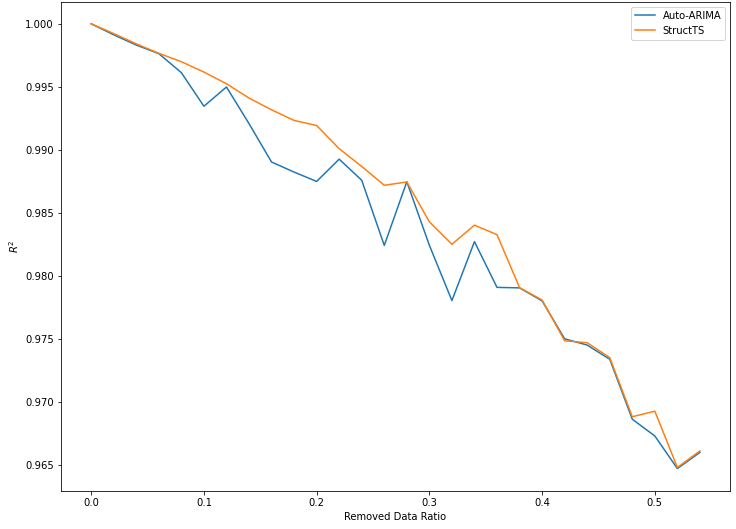
\includegraphics[width=\textwidth]{imp_traffic}
		\caption{Radio traffic load imputation}
		\label{fig:imp_radio_traffic}
	\end{subfigure}%
	\hfill
	\begin{subfigure}{.47\textwidth}
		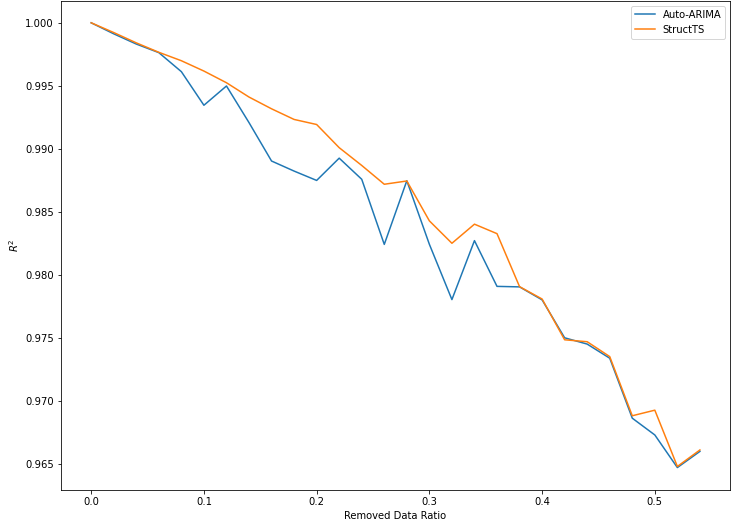
\includegraphics[width=\textwidth]{imp_temp}
		\caption{Cabinet temperature}
		\label{fig:imp_temp}
	\end{subfigure}
	\caption{Imputation experiments good results}
	\label{fig:imp_exp_good}
\end{figure}

Although the plots above show promising results, there are other cases where the experiment did not perform as expected. 

\pagebreak

\subsubsection*{Unintuitive $R^2$ values}

There are cases in which Auto-ARIMA estimation show poor and even negative $R^2$ values as shown in Figure \ref{fig:imp_exp_issue}. The latter are unintuitive results, as $R^2$ values are expected to be limited to the $[0,1]$ interval. 

Nonetheless, this is meant only for linear models, where the worst fitted model is assumed to be the observations mean[add citation]. Thus, having negative $R^2$ values implies that the observations mean explains more variance than the fitted model.

\begin{figure}[hptb]
	\begin{subfigure}{.47\textwidth}
		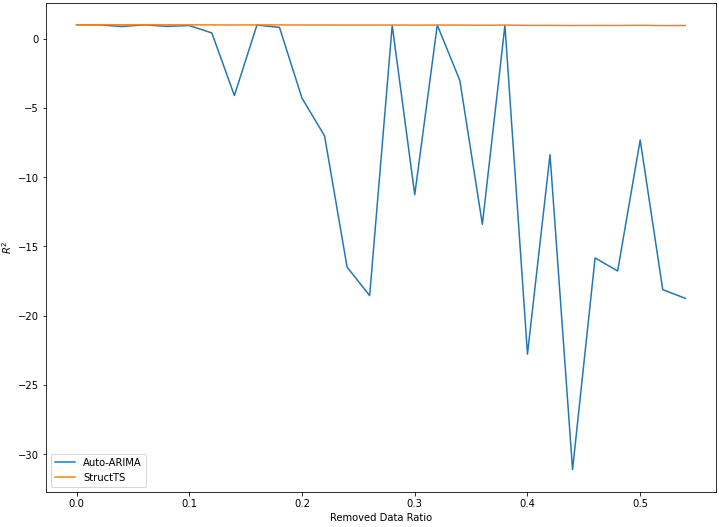
\includegraphics[width=\textwidth]{imp_sys_voltage}
		\caption{\ac{pdu} system voltage imputation}
		\label{fig:imp_pdu_sys_voltage}
	\end{subfigure}%
	\hfill
	\begin{subfigure}{.47\textwidth}
		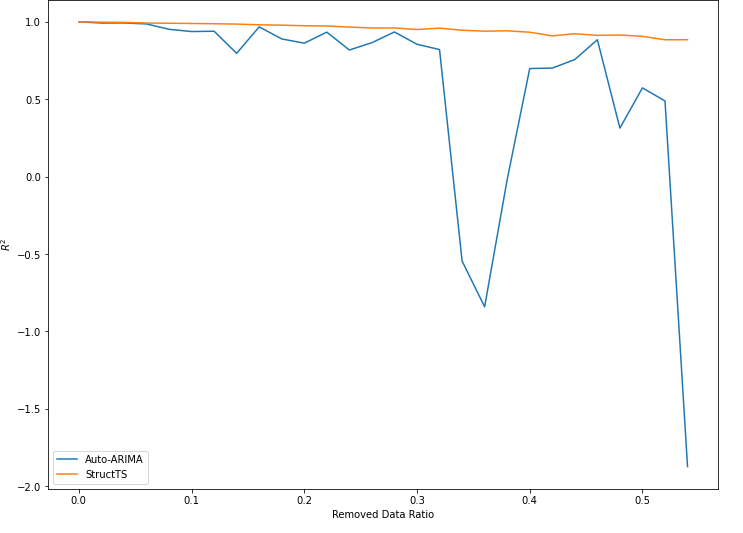
\includegraphics[width=\textwidth]{imp_power_load}
		\caption{Average \ac{psu} utilization imputation}
		\label{fig:imp_psu_load}
	\end{subfigure}
	\caption{Imputation experiments good results}
	\label{fig:imp_exp_issue}
\end{figure}

\subsubsection*{Optim convergence failures}

The model estimation threw runtime exceptions for some features due to the R code calls to the \texttt{optim} library not converging. These exceptions were found to be an actual bug in the library that occurs when the function being optimised tends to a constant value. 

A dedicated routine was written to catch whenever this exception was thrown and run a simple interpolation instead of estimating the model.

\begin{figure}[H]
	\centering
	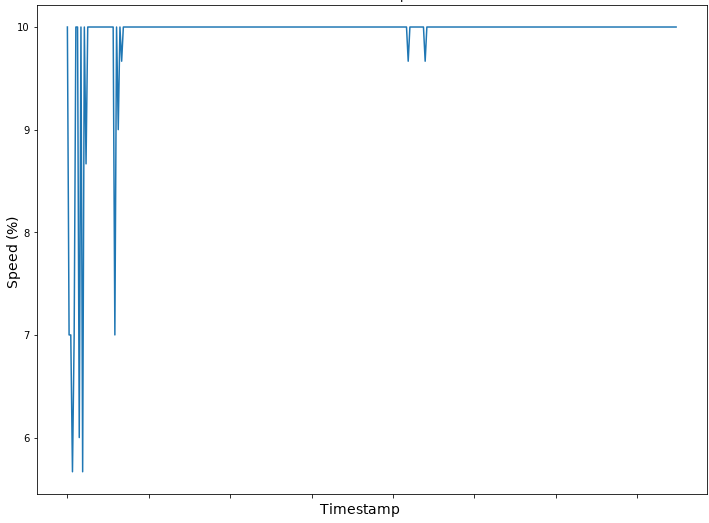
\includegraphics[width=0.55\linewidth]{imp_conv_issue}
	\caption{Problematic signals for imputeTS}
	\label{fig:imp_conv_issue}
\end{figure}

\section{Database construction algorithm}

It has been implemented a pipeline to build a unified and non-corrupted database from the sparsed raw files so that the forecasting section could learn from reliable data.

In the Figure, it is shown how the implemented blocks interact with each other to accomplish this task.

\begin{figure}[H]
	\centering
	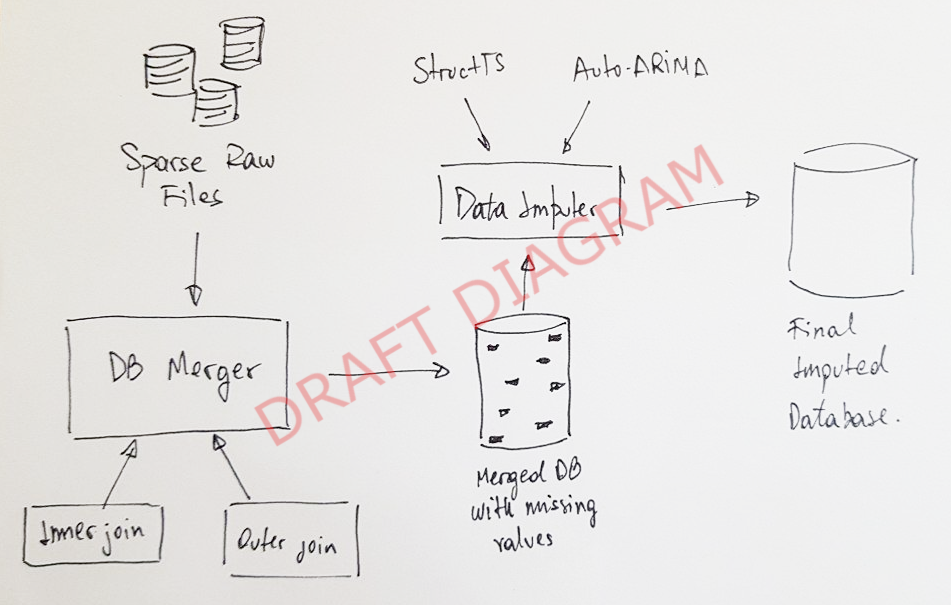
\includegraphics[width=0.65\linewidth]{db_construction_algorithm}
	\caption{Database construction algorithm}
	\label{fig:db_construction_algorithm}
\end{figure}


%
\chapter{Forecasting}
\label{cha:forecasting}

\section{Prophet}

\subsection{Model overview}

Prophet is a statistical model developed by engineers at Facebook, which mainly fits its models in Stan and has been open-sourced with public APIs for python and R languages\cite{fb_prophet}. It takes a regression-fitting approach to learn the time series and then forecasts by extrapolating such models and adding uncertainty in a Bayesian framework.

It uses a decomposable time series models \cite{harvey1990estimation} with three components: trend, seasonality and holidays:

\begin{equation}
	y(t) = g(t) + s(t) + h(t) + \varepsilon_t
\end{equation}

Where $g(t)$ is a trend function that models non-periodic fluctuations, $s(t)$ capture different kinds of seasonalities, and $h(t)$ represents special situations that could add irregularities to the other components and a random error term $\varepsilon$.

The model is similar to a \ac{gam}\cite{hastie1987generalized}, which allows adding more and more components as needed. The seasonalities are modelled by an exponential smoothing approach\cite{gardner1985exponential}.

\subsection{Trend model}

Prophet has two trend models: a saturating growth one, which is similar to model population growths in ecosystems \cite{hutchinson1978introduction} and a piecewise model to give the flexibility of trend changes in determined learnt changepoints \cite{fb_prophet}.

The basic saturated growth model is given by

\begin{align}\label{eq:sat_growth}
		g(t) &= \frac{C}{1 + \exp\left\{ -k(t-m) \right\}}
\end{align}

\begin{equation*}
	\text{Where} \quad
	C: \text{Carrying capacity}, \quad
	k: \text{Growth rate}, \quad
	m: \text{Offset parameter}
\end{equation*}

Nonetheless, the saturated growth model in (\ref{eq:sat_growth}) does not meet all the usual requirements for some of the applications in which the saturating ceiling varies over time or in which the growth rate is not constant. Therefore, the model has been extended as follows.

Let $s_j=1,\ldots,S$ be the number of changepoints where the growth rate is allowed to change. Then, let $\delta_j$ be the change rate that happens at $s_j$, and $\bm{\delta} \in \mathbb{R}^s$ the vector defined by all $\delta_j$. This means that the growth rate at any time $t$ is the base rate $k$ plus all the adjustments up to $t$

\begin{equation}
	k + \sum_{j=1}^{t < s_j}{\delta_j}
\end{equation}

This can be rewriten as

\begin{align}
	\begin{split}
		k &+ \bm{a}(t)^T\bm{\delta} \\
		\text{Where}\quad a_j &= 
		\begin{cases*}
			1\quad,\quad\text{if} \quad t > s_j \\
			0\quad,\quad\text{otherwise}
		\end{cases*}
	\end{split}
\end{align}

Also, when the growth rate is adjusted, the $m$ needs to be adjusted to ensure continuity. 

\begin{equation}
	\gamma_j = \left( s_j - m - \sum_{l<j}{\gamma_l} \right) \left(1 - \frac{k+\sum_{l<j}{\delta_l}}{k+\sum_{l \leq j}{\delta_l}} \right)
\end{equation}

Then the linear trend with changepoints is defined by (\ref{eq:piece_trend}) piecewise logistic growth model by (\ref{eq:piece_satgrowth})\cite{fb_prophet}.

\begin{equation}\label{eq:piece_trend}
	g(t) = \left( k + \bm{a}(t)^T \bm{\delta} \right)t + \left( m + \bm{a}(t)^T \bm{\gamma} \right)
\end{equation}

\begin{equation}\label{eq:piece_satgrowth}
	g(t) = \frac{C(t)}
	        {1 + \exp\left\{-(k+\bm{a}(t)^T\bm{\delta})(t-(m+\bm{a}(t)^T \bm{\gamma}))\right\}
	        }
\end{equation}


\subsection{Trend forecast}


After the model has learnt from a history of $T$ time points with $S$ changepoints from which each point has a rate change $\delta_j \sim \text{Laplace}(0,\tau)$. 

The trend will keep its last growth rate constant. The forecasts will be made by extrapolating the \ac{gam} and simulating samples from Laplace$(0,\lambda)$ where $\lambda$ is a variance inferred from the data from the maximum likelihood estimate of the rate scale parameter (\ref{eq:lambda_inferr}).

\begin{equation}\label{eq:lambda_inferr}
	\lambda = \frac{1}{2} \sum_{j=1}^{S}{|\delta_j|}
\end{equation}

Once $\lambda$ has been inferred the trend forecast and its uncertainty are obtained from

\begin{equation}\label{eq:trend_forecast}
\forall j > T\quad,\quad 
	\begin{cases}
		\delta_j = 0 \quad \text{w.p.} \frac{T-S}{S} \\
		\delta_j \sim \text{Laplace}(0,\lambda) \quad \text{w.p.} \frac{S}{T}
	\end{cases}
\end{equation}

\pagebreak
\subsection{Seasonalities}

By using the \ac{gam} flexibility, it is possible to add different seasonality periods, 365.25 or 7 for yearly and weekly seasonalities -in days measurements-, for example. These seasonalities are modelled by the use of Fourier series\cite{harvey_fourier}.

Therefore, for every given period $P$, it can be defined that.

\begin{equation}
	s(t) = \sum_{n=1}^{N}\left( a_n \cos\left( \frac{2 \pi n t}{P}\right)  + b_n \sin\left( \frac{2 \pi n t}{P}\right) \right)
\end{equation}

Which has $2N$ params to learn:

\begin{equation*}
	\bm{\beta} = \left[ a_1, b_1, a_2, b_2, \ldots, a_N, b_N\right]^T
\end{equation*}

In order to make the structures more manageable, it is defined a matrix of seasonalities comprised of the seasonal vectors for each time step.

\begin{equation}
	\bm{X}(t) = \left[ \cos\left( \frac{2 \pi (1) t}{P}\right), \sin\left( \frac{2 \pi (1) t}{P}\right), \dots , \cos\left( \frac{2 \pi (N) t}{P}\right), \sin\left( \frac{2 \pi (N) t}{P}\right)  \right]
\end{equation}

Thus, the seasonal component is expressed then as.

\begin{align}
	s(t) &= \bm{X}(t) \bm{\beta} \\
	\text{Where} \quad \beta &\sim \mathcal{N}(0, \sigma^2)
\end{align}


\subsection{Holidays and festivities}

Prophet also allows considering non-seasonal events that can significantly affect the forecasts due to changes in peoples behaviour. Namely, Muslim Ramadan, Chinese New Year or the US's Super Bowl.

It is assumed that each holiday is independent. For each holiday $i$, $D_i$ is the set of past and future dates of it. 

Same as seasonalities, a regressors matrix is generated indicating whether the time $t$ happens during holiday $i$ and a parameter $\kappa_i$ to model its influence in the forecast.

\begin{align}
	Z(t) &=  \left[   \bm{1}(t \in D_1), \ldots, \bm{1}(t \in D_L) \right] \\
	\therefore \quad h(t) &= Z(t)\bm{\kappa} \\
	\bm{\kappa} &\sim \mathcal{N}(0,\nu^2)
\end{align}

For practical cases, importing the holidays' dates can be done using the python-holidays open-source package \cite{Holidays}, for which an extract of available Swedish holidays is shown in Table \ref{table:sv_holidays}.

\begin{table}[H]
	\centering
	\begin{tabular}{|c|c|}
		\hline
		\textbf{Date} & \textbf{Holiday} \\
		\hline
		2021-01-01 &Nyårsdagen \\
		2021-01-06 &Trettondedag jul \\
		2021-04-02 &Långfredagen \\
		2021-04-04 &Påskdagen, Söndag \\
		2021-04-05 &Annandag påsk \\
		2021-05-01 &Första maj \\
		2021-05-13 &Kristi himmelsfärdsdag \\
		2021-05-23 &Pingstdagen, Söndag \\
		2021-06-06 &Sveriges nationaldag, Söndag \\
		2021-06-25 &Midsommarafton \\
		2021-06-26 &Midsommardagen \\
		2021-11-06 &Alla helgons dag \\
		2021-12-24 &Julafton \\
		2021-12-25 &Juldagen \\
		2021-12-26 &Annandag jul, Söndag \\
		2021-12-31 &Nyårsafton \\
		\hline
	\end{tabular}
	\caption{Results for Swedish holidays in 2021 from \texttt{python-holidays}}
	\label{table:sv_holidays}
\end{table}

It is possible also to include other parameters to extend the holiday to the neighbouring days. For more details, the reader can further investigate in \cite{fb_prophet}.

\subsection{Model fitting}

The seasonality and holiday components are then merged in a matrix $\bm{X}$ and the changepoints $\bm{a}(t)$, in a matrix $\bm{A}$. Then the model is expressed using Stan\cite{carpenter2017stan} as is shown in figure \ref{alg:stan}.

\begin{figure}[H]
\begin{lstlisting}
// Priors
k ~ normal(0, 5);
m ~ normal(0, 5);
epsilon ~ normal(0, 0.5);
delta ~ double_exponential(0, tau);
beta ~ normal(0, sigma);

// Logistic likelihood
y ~ normal(C ./ (1 + exp(-(k + A * delta) .* (t - (m + A * gamma)))) + X * beta, epsilon);

// Linear likelihood
y ~ normal((k + A * delta) .* t + (m + A * gamma) + X * beta, sigma);
\end{lstlisting}
\caption{Prophet Stan model.}
\label{alg:stan}
\end{figure}

Where \texttt{tau} and \texttt{sigma} are used to control the regularization levels.

Another handy feature that allows using \acp{gam} is to plot each component on its own, which allows the analyst to spot abnormalities when debugging a model. These plots will be shown and explained in the following sections.

\pagebreak
\subsection{Experiments}

The average \ac{psu} load signal shown in Figure \ref{fig:forecast_experiment_signal} has been chosen to run the following experiments. It is not a particularly easy signal since it contains some severe outliers in the first days that turned the power to almost zero, and at the end, the average power consumption seems to decrease.

It is necessary to notice that in every forecasting model, the longer the prediction horizon is, the more uncertainty and thus the lower performance. For this experiment, it has been decided to leave the last 10\% of data for testing purposes.

\begin{figure}[H]
	\centering
	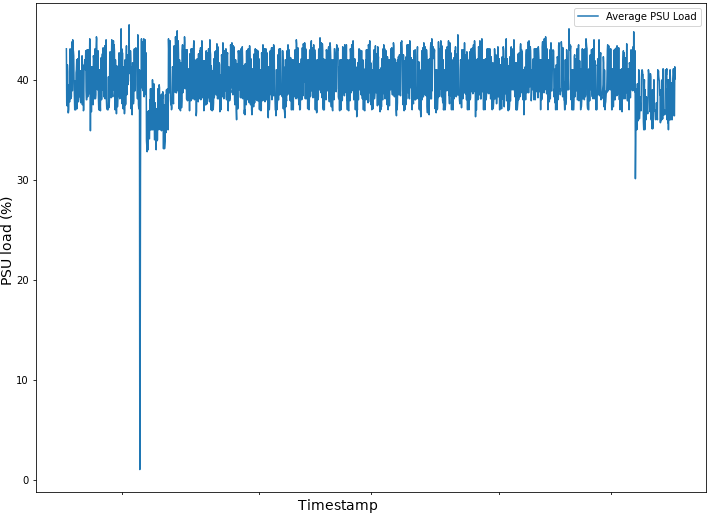
\includegraphics[width=0.6\linewidth]{forecast_experiment_signal}
	\caption{Signal used for the forecasting experiments}
	\label{fig:forecast_experiment_signal}
\end{figure}

In the following sections it is going to be shown first a pure univariate approach and later it will be added more exogenous regressors to improve the predictions. The models will be evaluated by using the following scores.

\subsubsection*{Coefficient of determination}

The coefficient of determination $R^2$ is a measure of how many variance of $\hat{y}$ is explained by the variance in $y$ in a linear regression context. It is compared against the considered \emph{worst possible linear approximation} which corresponds to the samples mean.

It is said that $R^2$ has values $[0,1]$, where $0$ corresponds to the worst linear model and 1 a perfect approximation. 

Althought the current application is not a linear regression case, $R^2$ is still considered a valuable score to compare predictor performances, nonetheless, as the linearity assumption is not met, its values would reside in $(-\infty, 1]$ where 0 still being the mean value, but it is no longer considered the worst possible fit.

\begin{equation}\label{eq:rsq}
R^2 = 1 - \frac{\sum_{i}{(y_i - \hat{y}_i)^2}}{\sum_{i}{(y_i - \bar{y}_i)^2}}
\end{equation}


\subsubsection*{Mean absolute error}

It measures, in absolute terms, the deviations from the true values. \ac{mae} is preferred, given its interpretability, over \ac{rmse} \cite{MAE}.

\begin{equation}\label{eq:mae}
\text{MAE}	= \frac{1}{N} \sum_{i=1}^{N}{ \left| y_i - \hat{y}_i \right| }
\end{equation}


\subsubsection*{Mean out-of-bounds error}

As result of the fitting process, prophet's output is comprised by the mean prediction $\hat{y}_t$ and also its lower and upper boundaries for a given confidence value when constructing the predictor object which defaults at $80\%$ 

Let then the \ac{obe} be the out-of-the-confidence-bands error defined by (\ref{eq:obe}) where $\Delta \hat{y}_t$ is the computed confidence interval half-magnitude for the time $t$. Then the \ac{mobe} can be obtained by taking the mean of these values to obtain an overall performance score as in (\ref{eq:mobe}). 

\begin{align}
\text{OBE}_i &= \bm{\min} \Big\{ \big| y_i - (\hat{y}_i - \Delta\hat{y}_i) \big| , \big	| y_i - (\hat{y}_i + \Delta\hat{y}_i) \big| \Big\} \label{eq:obe} \\
\text{MOBE} &= \frac{1}{N} \sum_{i=1}^{N}{ \text{OBE}_i }\label{eq:mobe}
\end{align}

\subsection{Univariate model implementation}

In the figure \ref{fig:prophet_uni_split} is shown the complete results of training and testing for a univariate prophet model.

\begin{figure}[H]
	\centering
	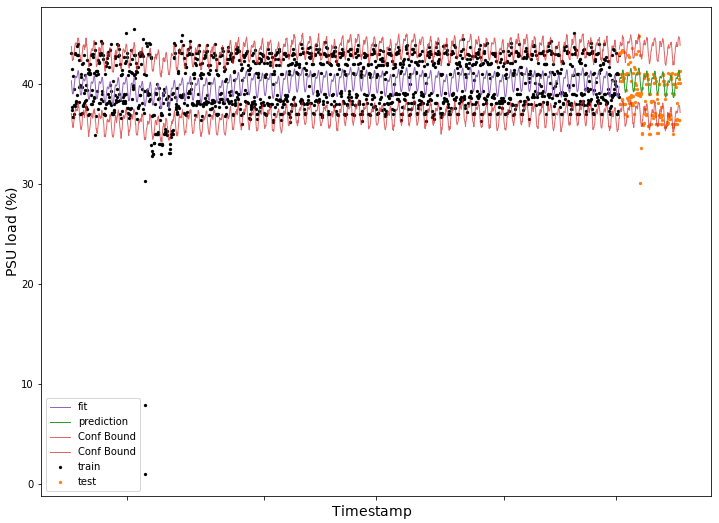
\includegraphics[width=0.6\linewidth]{prophet_uni_split}
	\caption{Training, test and predictions from univariate Prophet}
	\label{fig:prophet_uni_split}
\end{figure}

\subsubsection*{Training fitting}

In training is obtained a very poor $R^2$ value, which from the plot in figure \ref{fig:prophet_uni_fitting} can be expected, since $\hat{y}$ looks like mostly an average of the seasonal components. Nonetheless, if it is considered that predicting an interval is acceptable, then the \ac{mobe} shows a very good result. 

It can also be observed that the trend component did not overfit to the outliers.

\begin{table}[H]
	\centering
	\begin{tabular}{|c|c|}
		\hline
		\ac{mae} 	& 2.20 \\
		$R^2$ 		& 0.11 \\
		\ac{mobe} 	& 0.08 \\
		\hline
	\end{tabular}
	\caption{Univariate prophet training scores}
	\label{table:prophet_uni_train_scores}
\end{table}

\begin{figure}[H]
	\centering
	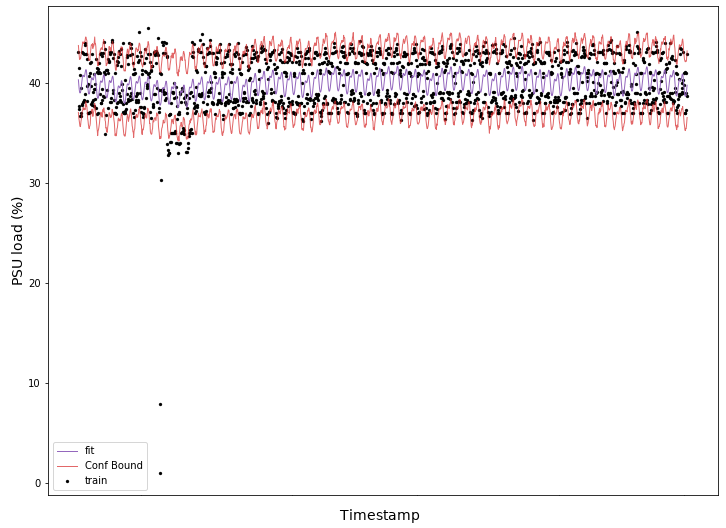
\includegraphics[width=0.6\linewidth]{prophet_uni_fitting}
	\caption{Training fitting from univariate prophet}
	\label{fig:prophet_uni_fitting}
\end{figure}

\subsubsection*{Model learnt components}

In figure \ref{fig:prophet_uni_components} it is shown the learnt approximation of every component in the \ac{gam}. Although the trend did not overfit to the outliers, still learnt that there is a break point and changed the piecewise trend.

\begin{figure}[H]
	\centering
	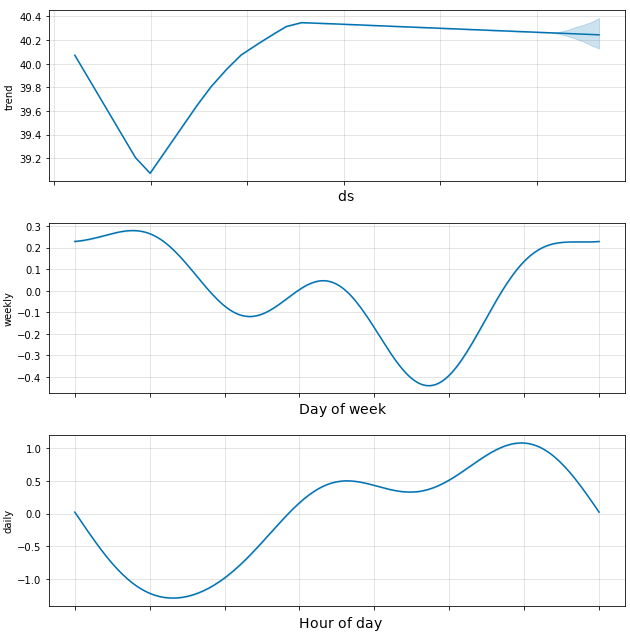
\includegraphics[width=0.7\linewidth]{prophet_uni_components}
	\caption{Learnt components from univariate prophet}
	\label{fig:prophet_uni_components}
\end{figure}

\pagebreak
\subsubsection*{Test predictions}

When it comes to the predictions performance, the $R^2$ shows even worse results. The \ac{mobe} is also high since the trend component was not able to foresee the decreasing in the middle of the test set as shown in figure \ref{fig:prophet_uni_preds}. 

\begin{figure}[H]
	\centering
	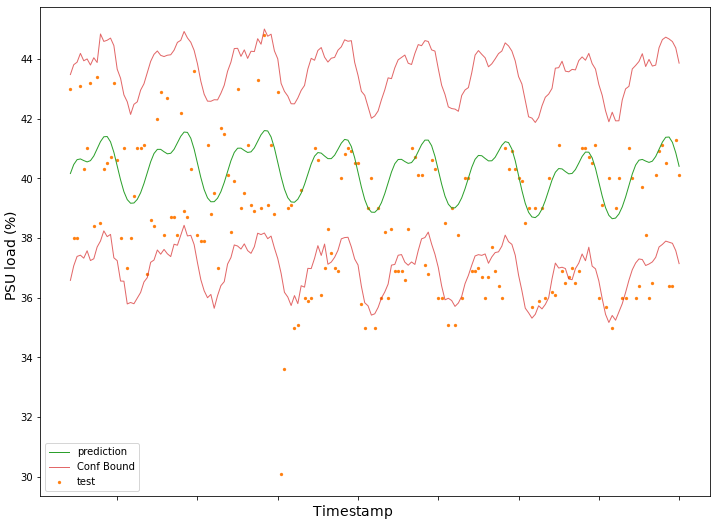
\includegraphics[width=0.6\linewidth]{prophet_uni_preds}
	\caption{Test predictions from univariate Prophet}
	\label{fig:prophet_uni_preds}
\end{figure}

\begin{table}[H]
	\centering
	\begin{tabular}{|c|c|}
		\hline
		\ac{mae} 	& 2.12 \\
		$R^2$ 		& -0.33 \\
		\ac{mobe} 	& 0.25 \\
		\hline
	\end{tabular}
	\caption{Univariate prophet prediction performance}
	\label{table:prophet_uni_test_scores}
\end{table}




\subsubsection*{Residual analysis}

The residuals in the training set still show somehow resembles the original data pattern. This could be interpreted that there is still patterns to learn from data, i.e., this model is not complete. 

\begin{figure}[hptb]
	\begin{subfigure}{.47\textwidth}
		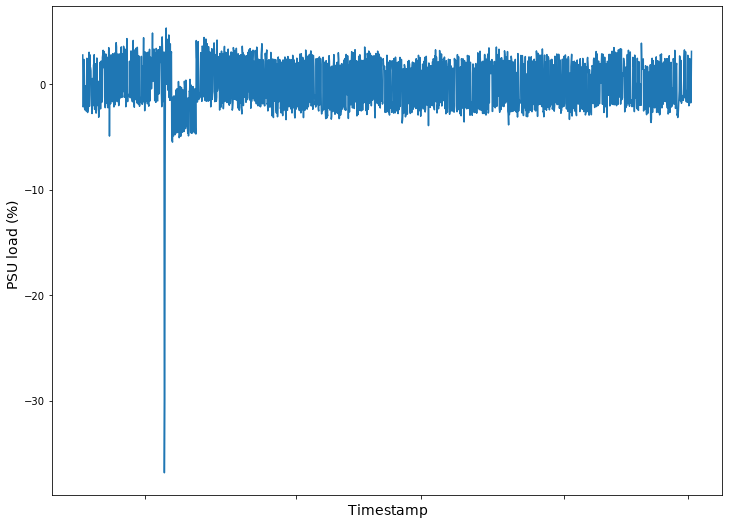
\includegraphics[width=\textwidth]{prophet_train_res_time}
		\caption{Residuals from train fit}
		\label{fig:prophet_train_res_time}
	\end{subfigure}%
	\hfill
	\begin{subfigure}{.47\textwidth}
		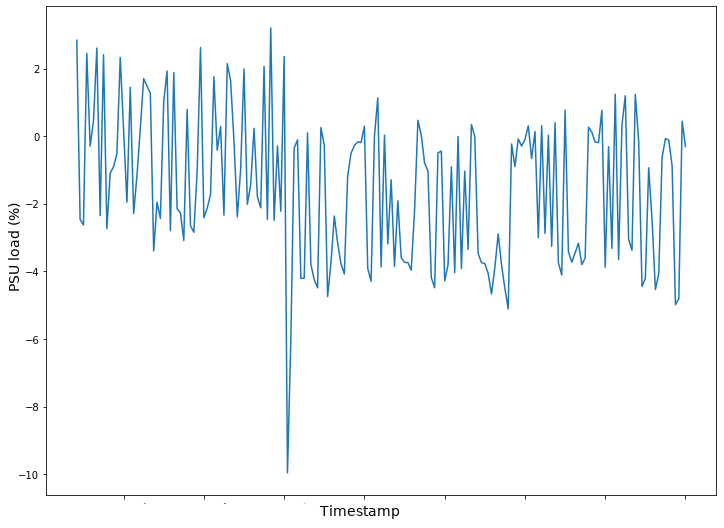
\includegraphics[width=\textwidth]{prophet_test_res_time}
		\caption{Residuals from test predictions}
		\label{fig:prophet_test_res_time}
	\end{subfigure}
	\caption{Univariate prophet residuals}
	\label{fig:prophet_res_time}
\end{figure}

Furthermore, if the joint distributions for $y$ and $\hat{y}$ are plotted, it can be seen how the outlier in the training set was not learnt and how the approximation becomes erratic in the test set.

\begin{figure}[hptb]
	\begin{subfigure}{.47\textwidth}
		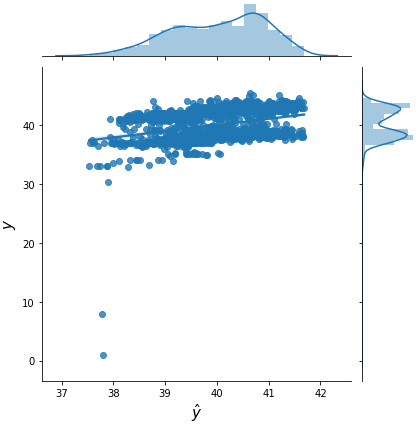
\includegraphics[width=\textwidth]{prophet_train_res_joint}
		\caption{Train}
		\label{fig:prophet_train_res_joint}
	\end{subfigure}%
	\hfill
	\begin{subfigure}{.47\textwidth}
		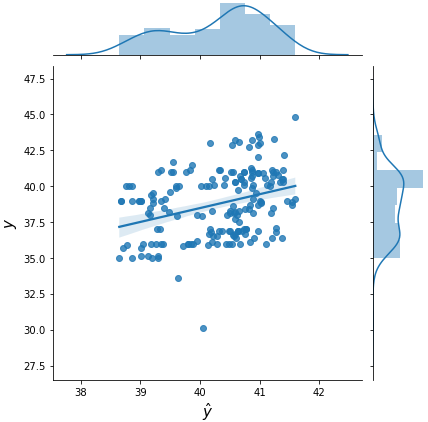
\includegraphics[width=\textwidth]{prophet_test_res_joint}
		\caption{Test}
		\label{fig:prophet_test_res_joint}
	\end{subfigure}
	\caption{Univariate prophet joint distributions of $y$ and $\hat{y}$}
	\label{fig:prophet_res_joint}
\end{figure}


\subsection{Implementation using exogenous regressors}

To fully exploit the flexibility of \acp{gam}, prophet's API allows defining custom regressors, which in the current work will be called exogenous variables as a resemblance of SARIMAX models. These variables are the ones explained in chapter \ref{cha:data_analysis}.



\subsubsection*{Model learnt components}

The model components now show the additive factor of all the exogenous regressors, which seems to contain the information not learnt by the univariate training residuals. 

\begin{table}[H]
	\centering
	\begin{tabular}{|c|c|}
		\hline
		\ac{mae} 	& 0.55 \\
		$R^2$ 		& 0.83 \\
		\ac{mobe} 	& 0.10 \\
		\hline
	\end{tabular}
	\caption{Multivariate prophet training scores}
	\label{table:prophet_multi_train_scores}
\end{table}

The $R^2$ score has considerably improved. Nonetheless, the other scores have become worse. The interpretation of this decline could be that the confidence band is now narrower than the univariate model. Thus, being out of the confidence band is now likely than before.

\begin{figure}[H]
	\centering
	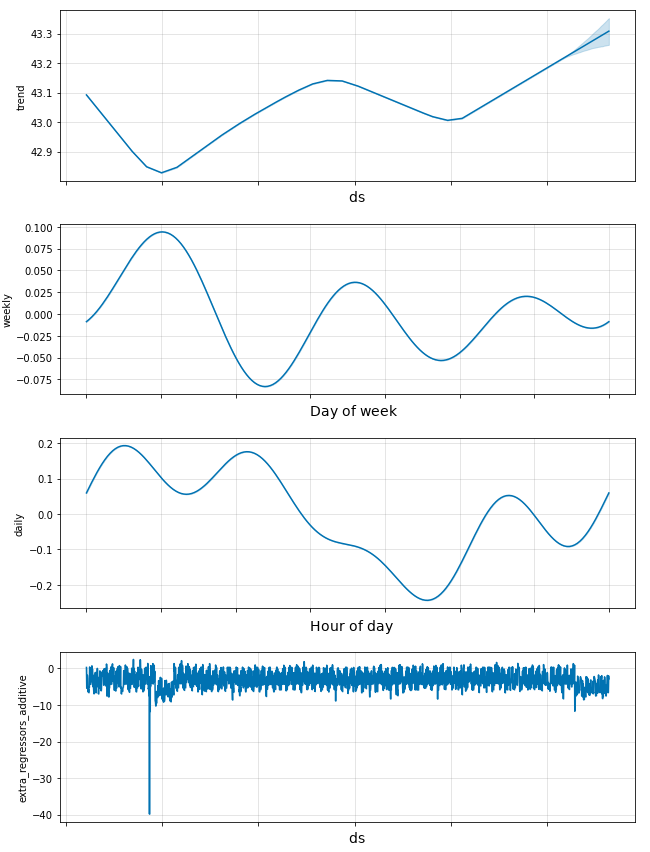
\includegraphics[width=0.7\linewidth]{prophet_multi_components}
	\caption{Learnt components from multivariate prophet}
	\label{fig:prophet_multi_components}
\end{figure}



\subsubsection*{Test predictions}

The results of the predictions have notoriously improved in this case. The $R^2$ value is close to 0.9, which for such a complex signal shows how powerful is the model. 

The \ac{mobe} has even decreased in the test set, this could be due to training outliers that still being difficult to approximate without overfitting the trend component. 

 
\begin{table}[H]
	\centering
	\begin{tabular}{|c|c|}
		\hline
		\ac{mae} 	& 0.52 \\
		$R^2$ 		& 0.88 \\
		\ac{mobe} 	& 0.05 \\
		\hline
	\end{tabular}
	\caption{Multivariate prophet prediction performance}
	\label{table:prophet_multi_test_scores}
\end{table}



\begin{figure}[H]
	\centering
	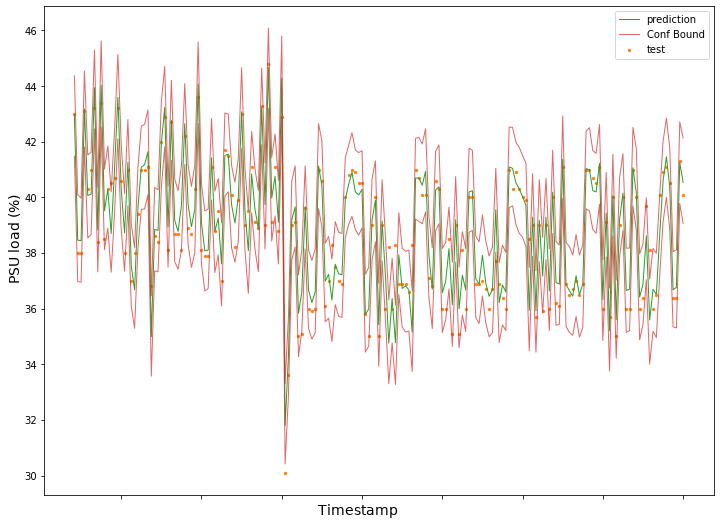
\includegraphics[width=0.6\linewidth]{prophet_multi_preds}
	\caption{Test predictions from multivariate prophet}
	\label{fig:prophet_multi_preds}
\end{figure}




\subsubsection*{Residual analysis}

The residuals now show that the patterns have been better learnt than in the univariate case.

\begin{figure}[hptb]
	\begin{subfigure}{.47\textwidth}
		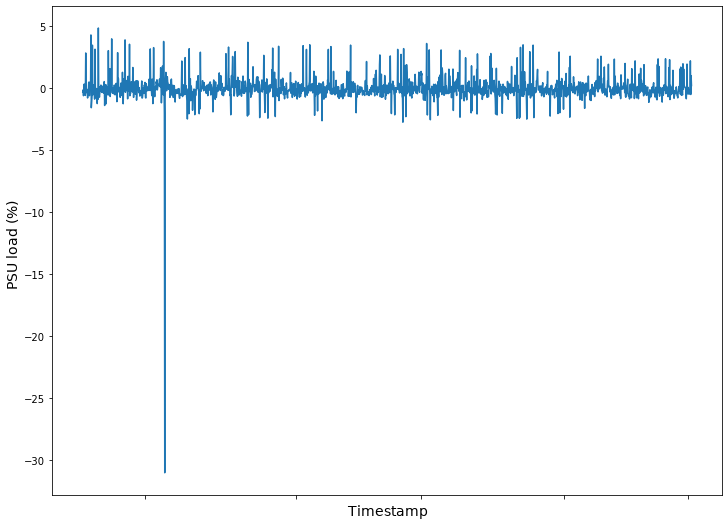
\includegraphics[width=\textwidth]{prophet_train_res_time_multi}
		\caption{Train}
		\label{fig:prophet_train_res_time_multi}
	\end{subfigure}%
	\hfill
	\begin{subfigure}{.47\textwidth}
		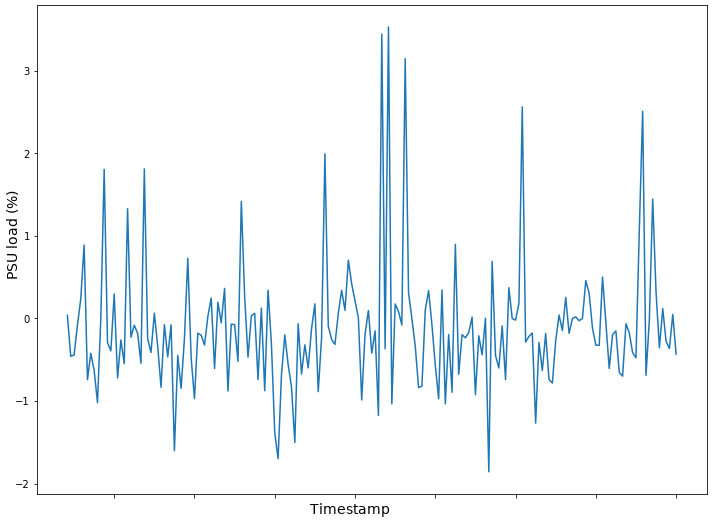
\includegraphics[width=\textwidth]{prophet_test_res_time_multi}
		\caption{Test}
		\label{fig:prophet_test_res_time_multi}
	\end{subfigure}
	\caption{Multivariate prophet residuals}
	\label{fig:prophet_res_time_multi}
\end{figure}

The joint distributions for $y$ and $\hat{y}$ now shows that the model is better approximating the signal. 

\begin{figure}[hptb]
	\begin{subfigure}{.47\textwidth}
		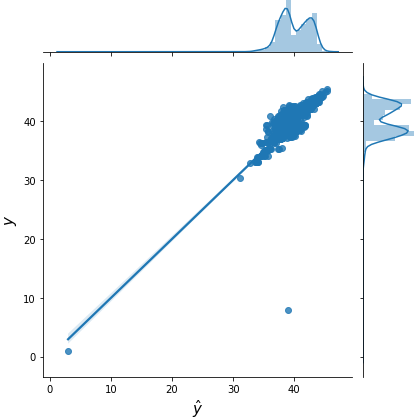
\includegraphics[width=\textwidth]{prophet_train_res_joint_multi}
		\caption{Train}
		\label{fig:prophet_train_res_joint_multi}
	\end{subfigure}%
	\hfill
	\begin{subfigure}{.47\textwidth}
		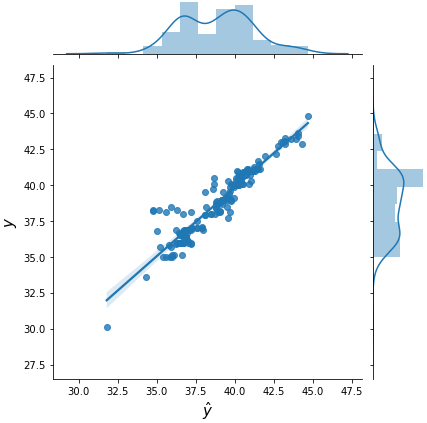
\includegraphics[width=\textwidth]{prophet_test_res_joint_multi}
		\caption{Test}
		\label{fig:prophet_test_res_joint_multi}
	\end{subfigure}
	\caption{Multivariate prophet joint distributions of $y$ and $\hat{y}$}
	\label{fig:prophet_res_joint_multi}
\end{figure}

%
%\pagebreak
%\section{Boosted random forests}
%
%
%\noindent\fbox{
%	\parbox{\textwidth}
%	{
%		Draft acknowledgement:\\
%		
%		The following models are still work in progress and last implementation has a bug to be fixed. 
%		
%		If time is not enough we may decide to drop this part for final report
%	}
%}
%
%\subsection{Model overview}
%
%\noindent\fbox{
%	\parbox{\textwidth}
%	{
%		Draft acknowledgement:\\
%		XGBoost regressor theory
%	}
%}
%
%\subsection{Regression approach}
%
%\begin{equation}
%	\label{xgb_reg}
%	y_{t+1} = \sum_{t=1}^{N}{\beta_t \cdot x_{t_i}}
%\end{equation}
%
%\begin{figure}[H]
%	\centering
%	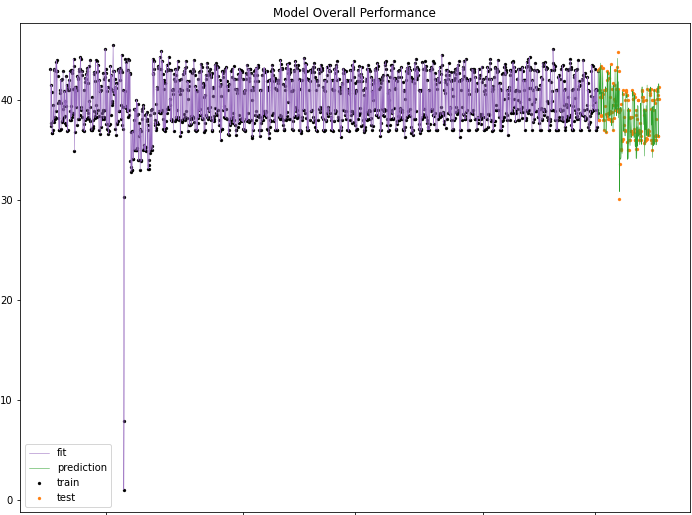
\includegraphics[width=0.6\linewidth]{xgb_reg_overall}
%	\caption{XGBoost overall performance}
%	\label{fig:xgb_reg_overall}
%\end{figure}
%
%\subsubsection*{Training fitting}
%
%\begin{figure}[H]
%	\centering
%	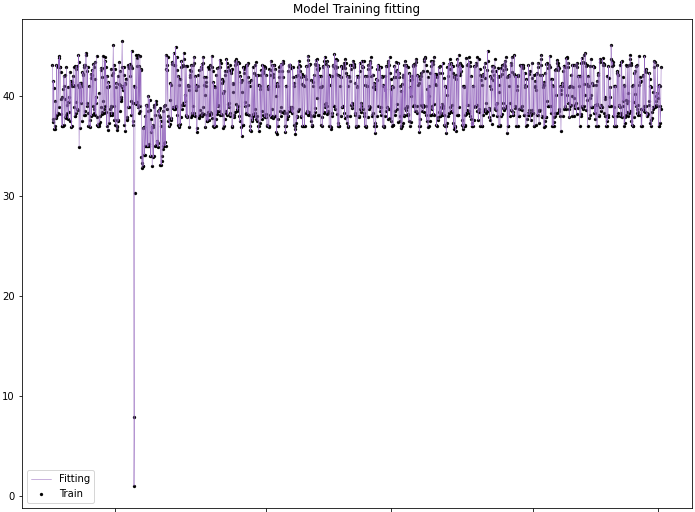
\includegraphics[width=0.6\linewidth]{xgb_reg_train}
%	\caption{XGBoost train performance}
%	\label{fig:xgb_reg_train}
%\end{figure}
%
%\begin{table}[H]
%	\centering
%	\begin{tabular}{|c|c|}
%		\hline
%		\ac{mae} 	& 0.04 \\
%		$R^2$ 		& 1.00 \\
%		\hline
%	\end{tabular}
%	\caption{XGBoost regressor train scores}
%	\label{table:xgb_reg_train_scores}
%\end{table}
%
%\subsubsection*{Test predictions}
%
%\begin{figure}[H]
%	\centering
%	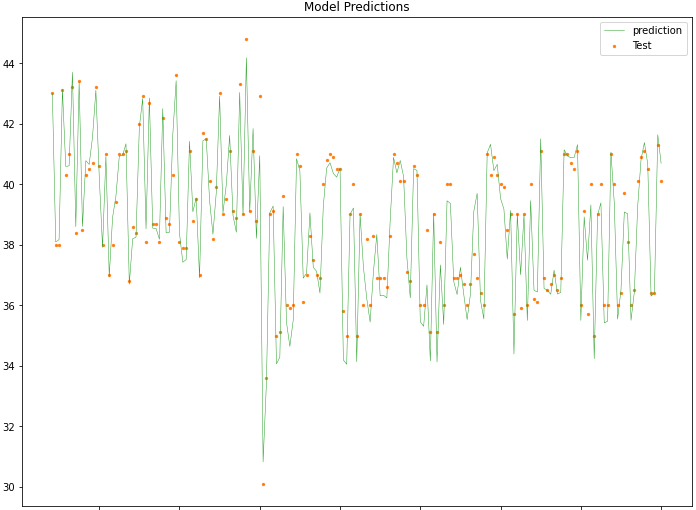
\includegraphics[width=0.6\linewidth]{xgb_reg_test}
%	\caption{XGBoost test performance}
%	\label{fig:xgb_reg_test}
%\end{figure}
%
%\begin{table}[H]
%	\centering
%	\begin{tabular}{|c|c|}
%		\hline
%		\ac{mae} 	& 0.44 \\
%		$R^2$ 		& 0.93 \\
%		\hline
%	\end{tabular}
%	\caption{XGBoost regressor prediction performance}
%	\label{table:xgb_reg_test_scores}
%\end{table}
%
%
%\subsubsection*{Residual analysis}
%
%\begin{figure}[hptb]
%	\begin{subfigure}{.47\textwidth}
%		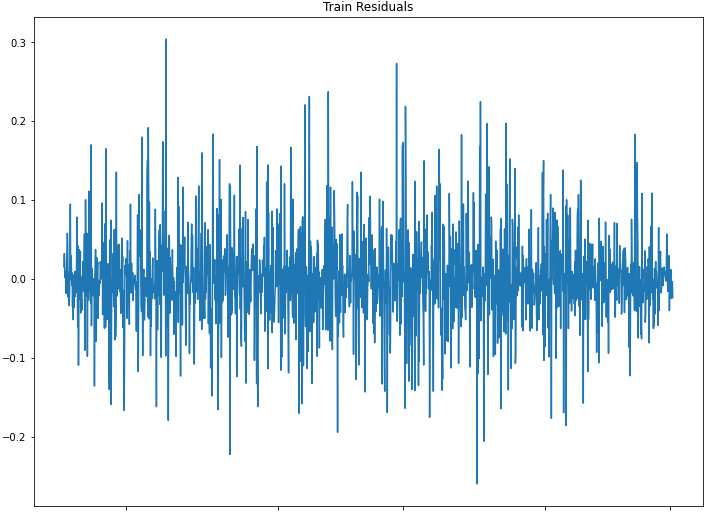
\includegraphics[width=\textwidth]{xgb_reg_res_train}
%		\caption{Train}
%		\label{fig:xgb_reg_res_train}
%	\end{subfigure}%
%	\hfill
%	\begin{subfigure}{.47\textwidth}
%		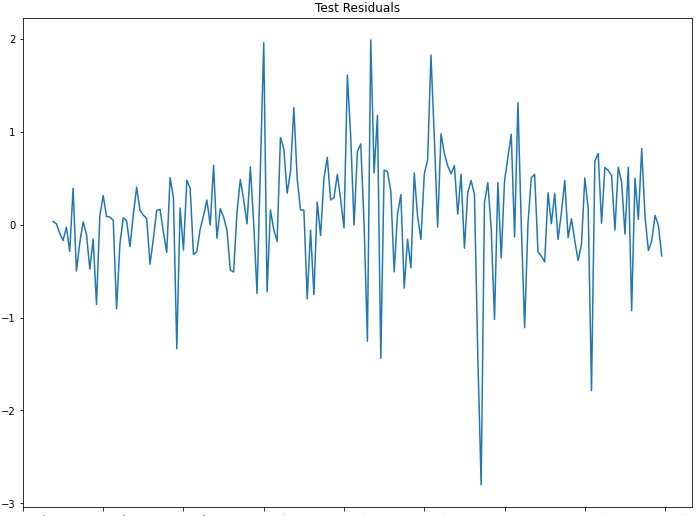
\includegraphics[width=\textwidth]{xgb_reg_res_test}
%		\caption{Test}
%		\label{fig:xgb_reg_res_test}
%	\end{subfigure}
%	\caption{XGBoost regression residuals}
%	\label{fig:xgb_reg_res}
%\end{figure}
%
%\begin{figure}[hptb]
%	\begin{subfigure}{.47\textwidth}
%		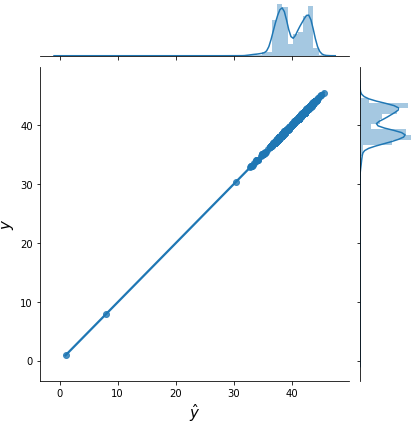
\includegraphics[width=\textwidth]{xgb_reg_joint_train}
%		\caption{Train}
%		\label{fig:xgb_reg_joint_train}
%	\end{subfigure}%
%	\hfill
%	\begin{subfigure}{.47\textwidth}
%		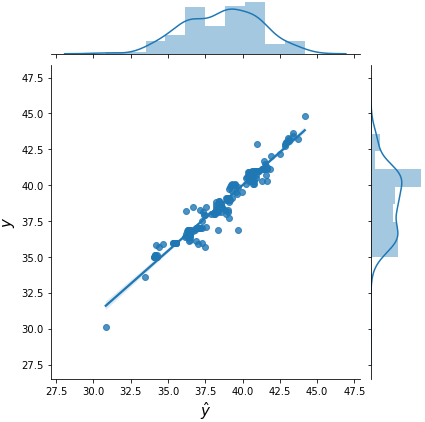
\includegraphics[width=\textwidth]{xgb_reg_joint_test}
%		\caption{Test}
%		\label{fig:xgb_reg_joint_test}
%	\end{subfigure}
%	\caption{XGBoost regression joint distributions of $y$ and $\hat{y}$}
%	\label{fig:xgb_reg_joint}
%\end{figure}
%
%\pagebreak
%\subsection{Including autoregressive components}
%
%Nonetheless, the function \ref{xgb_reg}, despite being trained to predict the next $y$ sample, still having only a regressive nature, i.e., no autoregressive components have been used to also learn from previous outputs. Thus, the function can be extended to:
%
%\begin{equation}
%	\label{xgb_ar}
%	y_{t} = \sum_{i=1}^{N}{\beta_i \cdot x_{{t-1}_i}} + \sum_{l=1}^{L}{\phi_l \cdot y_{t-l}}
%\end{equation}  
%
%Where $N$ is the amount of features and  $L$ corresponds to the amount of lags under consideration.
%
%\subsubsection*{Provisional results}
%
%\noindent\fbox{
%	\parbox{\textwidth}
%	{
%		Draft acknowledgement:\\
%		This section has a bug, which fixing will be resumed as soon as the report draft is delivered
%	}
%}
%
%\begin{figure}[H]
%	\centering
%	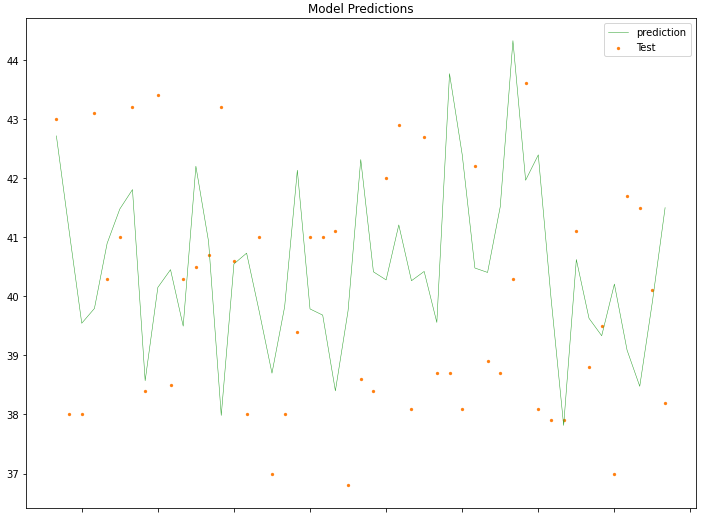
\includegraphics[width=0.6\linewidth]{xgb_ar_test}
%	\caption{XGBoost with autoregressive components test performance}
%	\label{fig:xgb_ar_test}
%\end{figure}
%
%\begin{figure}[hptb]
%	\begin{subfigure}{.47\textwidth}
%		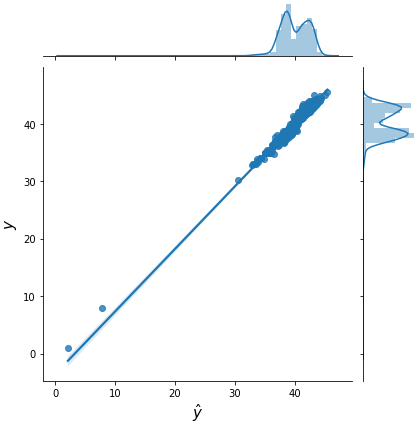
\includegraphics[width=\textwidth]{xgb_ar_joint_train}
%		\caption{Train}
%		\label{fig:xgb_ar_joint_train}
%	\end{subfigure}%
%	\hfill
%	\begin{subfigure}{.47\textwidth}
%		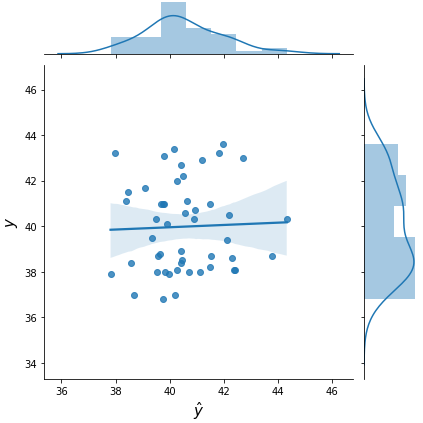
\includegraphics[width=\textwidth]{xgb_ar_joint_test}
%		\caption{Test}
%		\label{fig:xgb_ar_joint_test}
%	\end{subfigure}
%	\caption{XGBoost with autoregressive components joint distributions of $y$ and $\hat{y}$}
%	\label{fig:xgb_ar_joint}
%\end{figure}

%
\chapter{Power headroom estimation}

Until this point of the work, the research has been mainly focused on PSU loads forecasting. Nonetheless, as mentioned in the introductory context, the goal is to predict the power headroom defined in (\ref{eq:phdroom}). But as there are no direct measurements of power headroom that can be learnt, it is needed to derive it from the power consumption. 

Therefore, to provide a power headroom forecast, after estimating the future values of the loads' consumptions, it is needed a further step to translate that information into power headroom terms.

The following sections will propose a way to manage to achieve it and discuss other aspects of its technical applicability.

\section{Power headroom derivation as PSU utilisation complement}

As it has been exposed in section \ref{subsec:data_description:power_supply}, the power load is a measure of \emph{how many percentual power capacity it is being used at that time}. Thus, it is straightforward to claim that the percentual power headroom is its complement.

If the interest is to obtain a measurement in Watts units, the installed power capacity in the RBS, $P_{max}$, is needed to be known so that its proportion can be computed as follows.

\begin{align}\label{eq:ph_deriv}
\begin{split}
		P_{h[\%]}	&= 100 - P_{L[\%]} \\
		\text{Where }P_{h[\%]}	&: \text{Power headroom in percents} \\
		\text{and } P_{L[\%]}	&: \text{Power loads consumptions in percents}
\end{split}
\end{align}

If the interest is to obtain a measurement in Watts units, it is needed to know the installed power capacity, $P_{max}$, in the RBS so that its proportion can be computed as showed in (\ref{eq:phwatts}).

\begin{align}\label{eq:phwatts}
\begin{split}
		P_h	&= P_{max} \cdot \frac{P_{h[\%]}}{100} \\
	\text{Where } P_{max}	&: \text{Installed power capacity in Watts}
\end{split}
\end{align}

As an example, let the power load be the signal used in the forecast in chapter \ref{cha:forecasting}, and assume the installed power in the current \ac{rbs} is $12[kW]$. Then, the obtained curves are presented in Figure \ref{fig:ph_der}.

\begin{figure}[hptb]
	\centering
	\begin{subfigure}{.6\textwidth}
		\centering
		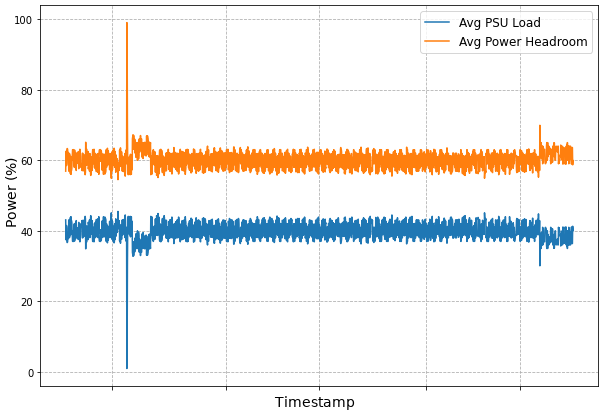
\includegraphics[width=\textwidth]{power_headroom_derivation}
		\caption{Derived power headroom in percents}
		\label{fig:ph_der_percent}
	\end{subfigure}%
	\hfill
	\begin{subfigure}{.6\textwidth}
		\centering
		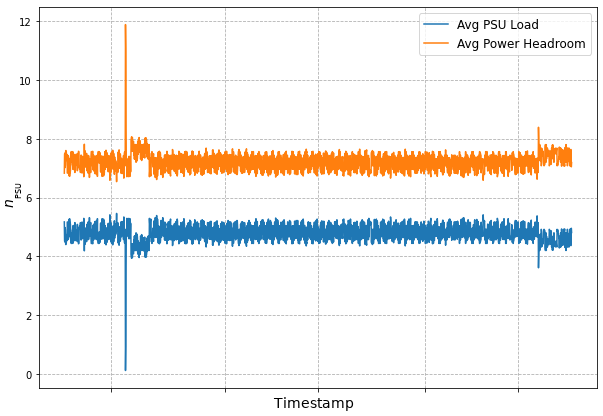
\includegraphics[width=\textwidth]{power_headroom_derivation_watts}
		\caption{Derived power headroom in Watts}
		\label{fig:ph_der_watts}
	\end{subfigure}
	\caption{Power headroom derivation from PSU Load}
	\label{fig:ph_der}
\end{figure}

\section{Criterion considerations}

In general terms, an alarm is meant to notice that something abnormal is happening in a process or, in a forecasting context, may (or will) occur in the future and support the operator response\cite{iec_alarms}.

In the current works' context, the alarm meaning can be conceived as the RBS not having enough power to manage to keep its by-design behaving.

Although it should be possible to define how likely a power overload is given the system's current state in probability terms, triggering an alarm is a binary task. The system is operating either in a \emph{"safe"}  or in an \emph{"abnormal"} region. Then crossing a boundary that separates these two regions is the trigger for the alarm. 

There are different techniques to tune an optimal trigger level. It could be done based on a system variable, or a latent variable or even a joint distribution of the two kinds\cite{izadi2009alarms}. 

Choosing the best possible boundary is considered to be out of the current work scope. Nonetheless, as an initial approach, it can be proposed to be settable by the user according to their needs and expertise. 

From this assumption and the derivations in (\ref{eq:ph_deriv}) and (\ref{eq:phwatts}) the following guidelines should be taking into consideration. 

\subsubsection*{Values interpretation}

Percentages values are not always able to fully represent the system conditions. For example, it is very different having 10\% of power headroom where the total capacity is 100 [kW] and 1 [kW] since the relative oscillations could be drastically different. Therefore, the power magnitude should be taken into consideration. 

\subsubsection*{PSUs do not partially fail}

The power capacity is not continuous. It will have discrete values as shown in Figure (\ref{fig:ph_lvls}), and also, the \acp{psu} can have different power contributions. This means that in order to set the threshold is needed to take into account the worst-case scenario, which would be \emph{"can the \ac{rbs} work if the next failure is the most power contributing \ac{psu}"}.


\begin{figure}[hptb]
	\centering
	\begin{subfigure}{.6\textwidth}
		\centering
		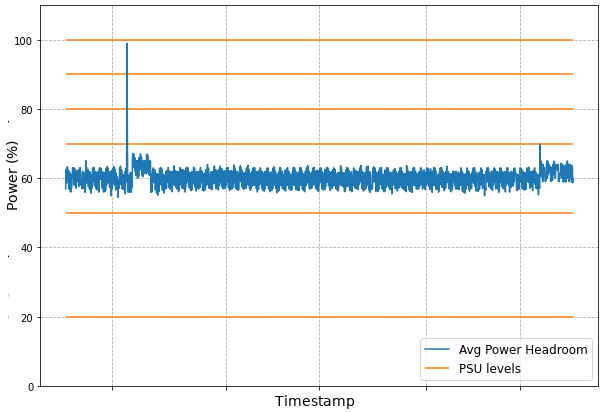
\includegraphics[width=\textwidth]{power_headroom_levels_percent}
		\caption{Power headroom and discrete availability in percents}
		\label{fig:ph_lvls_percent}
	\end{subfigure}%
	\hfill
	\begin{subfigure}{.6\textwidth}
		\centering
		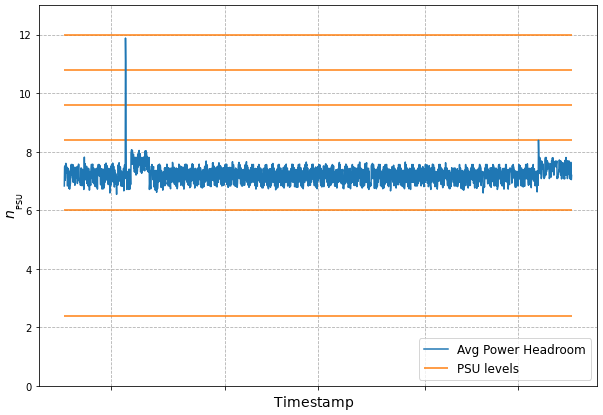
\includegraphics[width=\textwidth]{power_headroom_levels_watts}
		\caption{Power headroom and discrete availability in Watts}
		\label{fig:ph_lvls_watts}
	\end{subfigure}
	\caption{Power headroom derivation from PSU Load}
	\label{fig:ph_lvls}
\end{figure}

\pagebreak

\section{The $n$-level safety criteria}
Putting into mathematics the worst-scenario premise:

Let $N$ be the amount of PSUs installed, let $P_{PSU_1}, \ldots, P_{PSU_N}$ be the highest and the lowest power contribution from a working PSU, respectively. Then, let the $n$-level safety criteria, be the amount of worst-case \ac{psu} failures to have as operational margin:

\begin{align}
\begin{split}
	P_{max} - \sum_{i=1}^{n}{P_{PSU_i}} &> \bar{P}_{Load} + \Delta p \\
	P_{max} - \left\{\bar{P}_{Load} + \Delta p \right\} &> \sum_{i=1}^{n}{P_{PSU_i}}
\end{split}
\end{align}

But, as the power headroom is by definition the diference between the installed power capacity and the power being consumed. 

\begin{align}
	\begin{split}
		P_{h} &= P_{max} - \left\{\bar{P}_{Load} + \Delta p \right\} \\
		P_{h} &> \sum_{i=1}^{n}{P_{PSU_i}} \\
		\therefore P_{n-critical} &= \sum_{i=1}^{n}{P_{PSU_i}}
	\end{split}
\end{align}

Where $\Delta p$ is the confidence interval used when training the Prophet model.





\chapter{Methods}
\label{cha:method}

\section{Overall pipeline architecture}

By joining all the parts exposed in the previous chapters, the resulting pipeline proposed as a solution is shown in Figure \ref{fig:sol_pipeline}. Based on the flow presented, the obtained results are summarised in the following sections.

\begin{figure}[H]
	\centering
	\includegraphics[width=1\linewidth]{pipeline_v4}
	\caption{Overall pipeline architecture}
	\label{fig:sol_pipeline}
\end{figure}


\section{Database building and time series merging}
\label{sec:db_building}

As mentioned, the data is sparse across several files depending on its domain. Therefore, all the data has been merged into one consolidated database to make it more manageable to handle. Then, there is the problem of determining the best approach to join all these data without corrupting its integrity as a valid time series; this means having an invariant sampling time with fully defined observations vectors.

Among the data tables, it can be seen that the two fields that are always present, and therefore are suitable to use as keys to index all the different tables and join them, are the timestamp of the sample and the \ac{rbs} that has produced it. Therefore, the tuples $(\text{date}_i, \text{rbs}_i)$ will be used as keys. This means, having two relations $R(x_1, \ldots, x_n)$ and $S(y_1,\ldots,y_m)$ a third relation could be constructed $Q(z_1, \ldots, z_k) = R \times S$ such that $R(\vec{x}_i) = S(\vec{y}_i$) be the keys \cite{mishra1992join}.

\begin{figure}[H]
	\centering
	\includegraphics[width=0.55\linewidth]{db_merge_pipeline.png}
	\caption{Database consolidation}
	\label{fig:db_merge}
\end{figure}

In an ideal situation, all the time series for a given \ac{rbs} would have no missing data and identical timestamps, so just intersecting them would result in a complete-time series with equal sampling time, and no information would be lost.  Nonetheless, that is not the current case. As real-world data, technical issues happen now and then. There could be missing samples, or the timestamps between different files are not equidistant and, therefore, a join using them will not perform as expected.

The present work has been implemented mainly in Python with a few exceptions in R. The joining part is not an exception; thus, pandas \texttt{merge} options are available to use: \emph{left, right, outer, inner} or \emph{cross}. Merge operations in pandas work on two sets \cite{reback2020pandas}. Thus, for joining multiple series, successive two-sided \texttt{merge} operations have to be performed.

\subsection{Strategy analysis: Inner join}

An inner join constitutes an intersection between both sets. The implementation in pandas allows indicating the keys to be intersected, and as a result, a tuple is returned containing the matched keys with the remaining members. This can be expressed as the following 

$$Q(date_i, rbs_i,  x_{i_1}, \ldots, x_{i_n}, y_{i_1}, \ldots, y_{i_m}) = $$
$$  R(date_i, rbs_i, x_{i_1}, \ldots, x_{i_n}) \bigcap \
S(date_i, rbs_i, y_{i_1}, \ldots, y_{i_m}) $$

Furthermore, in a more programming-friendly manner, it can also be expressed as a SQL query. The expression above would be as the following and graphically as a 3D Venn diagram as in Figure \ref{fig:inner_join}.

\begin{lstlisting}[language=SQL]
SELECT * 
FROM R 
INNER JOIN S
ON R.date = S.date AND R.rbs = S.rbs;
\end{lstlisting}

The most significant disadvantage of this strategy relies on losing the observations that are not indexed in both datasets. Such nuisance will imply losing the series' head and tails if both series do not have the same start and finish times. If the missing samples are within the series, it will corrupt the constant sampling constraint. Given the amount of data available, these are situations to be avoided.  

\begin{figure}[H]
	\centering
	\includegraphics[width=0.90\linewidth]{join_inner}
	\caption{Inner join}
	\label{fig:inner_join}
\end{figure}

 

\subsection{Strategy analysis: Outer join approach}

Whereas an inner join implies an intersection, an outer join can be understood as a union. In pandas, the union implementation is performed in the keys domain, and the rest of the vector is preserved.  If there is some missing value in terms of samples or the full covariates, \texttt{NaN} will be used to fill in.

Given the relations $R$ and $S$ from Section \ref{sec:db_building}:

$$R(date_i, rbs_i, x_{i_1}, \ldots, x_{i_n}), S(date_i, rbs_i, y_{i_1}, \ldots, y_{i_m})$$

The resulting \emph{outer-joined} relation $Q$ on keys $(\text{date}_i, \text{rbs}_i)$

$$Q(date_i, rbs_i) = R(date_i, rbs_i) \bigcup S(date_i, rbs_i)$$

Such that the missing values on each of the relations are declared as NaN

$$Q(x_i) = \text{NaN} , \forall R(y_i) : (date_i, rbs_i) \in S \land (date_i, rbs_i) \notin S$$
$$Q(y_i) = \text{NaN} , \forall S(x_i) : (date_i, rbs_i) \in R \land (date_i, rbs_i) \notin R$$

Again, in a more programming-friendly fashion, the SQL query would look like the following and a more explanatory Venn diagram as in  \ref{fig:outer_join}.

\begin{lstlisting}[language=SQL]
SELECT *
FROM R
FULL OUTER JOIN S
ON R.date = S.date AND R.rbs = S.rbs;
\end{lstlisting}


\begin{figure}[H]
	\centering
	\includegraphics[width=0.90\linewidth]{join_outer}
	\caption{Outer join}
	\label{fig:outer_join}
\end{figure}

The drawback of this approach is related to its insertion of NaNs, which will imply either postprocessing after merging all the time series or preprocessing before the learning stage.

\subsection{Chosen strategy}

Given the analysis, it has been decided that not losing information is more critical than having to dedicate efforts to postprocessing it later to handle the non-computable values. Therefore, the outer join approach will be used for the following steps.

\section{Data Imputation}

As in the previous step, and based on time constraints, it has been decided not to implement algorithms from scratch but rely on existing known packages to avoid investing in developing time. 

Moritz et al. have analysed several univariate time series imputation implementations in R \cite{MoritzComparison}, which results later have been compiled in the \texttt{imputeTS} R package \cite{imputeTS}. Therefore, it is reasonable to rely on their work and use their results to decide which imputing strategy should be taken. 
Thus, for the current work, the \texttt{imputeTS} package will estimate a structural time series model from the data and then perform the Kalman smoothing to fill the gaps. 

It should be noted that before performing the Kalman smoothing, a state representation of the model is needed, \texttt{imputeTS} supports Auto-ARIMA state-space estimation and structural time series model fitted by maximum likelihood. In addition, it should be mentioned that the development has been mainly done in Python. Nonetheless, for this phase, an R package will be called from Python using the \texttt{rpy2} module as an interface to bounce between both languages.

\subsection{Auto-ARIMA algorithm}

Despite the fact that in the library the procedure is called \emph{auto-ARIMA}, it does also support SARIMA models.

The main goal of auto-tuning these models is to choose the appropriate $p, q, d, P, Q$ and $D$ values so the model can make a good approximation of the process. If $d$ and $D$ are known, $p, q, P, Q$ can be selected by using an information criterion such as the \ac{aic} \cite{Akaike1998}:

\begin{equation}
	\text{AIC} = -2\log(L) + 2(p+q+P+Q+k)
\end{equation}

Where $k=1$ if $c\neq0$ in equation (\ref{eq:sarima}) and $0$ otherwise, and $L$ is the maximised likelihood of the model fitted to $(1-B)^d (1-B^s)^D \{Y_t\}$ \cite{autoarimaLib}.  

\texttt{ImputeTS} library does not implement the (S)ARIMA estimation. Instead, it uses the \texttt{forecast} package for it \cite{imputeTS}.

The \texttt{forecast} library implements the Hyndman-Khandakar algorithm for \ref{eq:sarima}, which uses an heuristic that combines unit root tests, \ac{aic} minimisation and MLE maximisation as shown in Figure \ref{alg:autoarima} which is a transcription, in form of a DFD diagram, of the algorithm the authors have described in \cite{autoarimaLib}.

\begin{figure}[h]
	\centering
	\includegraphics[width=\linewidth]{autoarima_algo}
	\caption{Hyndman-Khandakar algorithm for Auto-ARIMA estimation}
	\label{alg:autoarima}
\end{figure}
 
% \begin{figure}[H]
% 	\noindent\fbox{
% 		{\small\parbox{\textwidth}
% 			{
% 				\subsubsection*{Step 1: Find $D$ and $d$}
% 				
% 				For non-seasonal data run KPSS unit-root tests \cite{kpss}. If the results are significant difference the data and repeat $d$ times until the test results are insignificant. 
% 				
% 				For seasonal data it is considered ARIMA$(p,d,q)(P,D,Q)_s$ models where $s$ is the seasonal frequency and $D=0$ or $D=1$ depending on a extended Canova-Hansen test \cite{canovahansen} (for $s$ > 13 the library estimates critical values $C_s = 0.269s^{0.928}$). 
% 				
% 				After the seasonal pattern has passed its stability test and $D$ has been selected, $d$ is chosen by successive KPSS tests for seasonal differenced data if $D=1$, or the original data if $D=0$
% 				
% 				\subsubsection*{Step 2: Initial model}
% 				
% 				Fit the following models
% 				
% 				\begin{itemize}
% 					\item ARIMA$(2,d,2)$ if $s=1$ or ARIMA$(2,d,2)(1,D,1)$ if $s \geq 1$
% 					\item ARIMA$(0,d,0)$ if $s=1$ or ARIMA$(0,d,0)(0,D,0)$ if $s \geq 1$
% 					\item ARIMA$(1,d,0)$ if $s=1$ or ARIMA$(1,d,0)(1,D,0)$ if $s \geq 1$
% 					\item ARIMA$(0,d,1)$ if $s=1$ or ARIMA$(0,d,1)(0,D,1)$ if $s \geq 1$
% 				\end{itemize}
% 				
% 				From these ones it is selected the one with lowest AIC score as initial model, it will be called \emph{current} model and denoted as ARIMA$(p,d,q)$ if $s=1$ or ARIMA$(p,d,q)(P,D,Q)_s$ if $s \geq 1$
% 				
% 				\subsubsection*{Step 3: Explore variations}
% 				
% 				13 variations of current model are explored. They are summarised as: 
% 				
% 				\begin{itemize}
% 					\item One of $p, q, P$ and $Q$ is allowed to vary by $\pm1$ from the current model
% 					\item $p$ and $q$ vary both $\pm1$ from the current model
% 					\item $P$ and $Q$ both vary by $\pm1$ from the current model
% 					\item $c$ is included if the current model has $c=0$ or excluded if the current model has $c\neq0$.
% 				\end{itemize}
% 				
% 				Once it is found a model with better AIC score than the current model, then this one is updated. The algorithm stops when no better AIC than the current is found. 
% 				
% 				
% 				\emph{Note: The model updating is also subjected to stability constraints that can be found in the original publication for further details.}
% 				
% 			}
% 	}}
% 	\caption{Hyndman-Khandakar algorithm for Auto-ARIMA estimation}
% 	\label{alg:autoarima}
% \end{figure}


\section{Database construction pipeline}


A pipeline has been implemented to build a unified and non-corrupted database from the sparse-raw files so that the forecasting section could learn from reliable data. Figure \ref{fig:db_construction_algorithm} shows how the implemented blocks interact with each other to accomplish this task.

\begin{figure}[H]
	\centering
	\includegraphics[width=0.8\linewidth]{db_construction_algorithm_final}
	\caption{Database construction algorithm}
	\label{fig:db_construction_algorithm}
\end{figure}







\section{Prophet fitting}

Prophet's Stan core \cite{carpenter2017stan} can be found in their GitHub repository\footnote{https://github.com/facebook/prophet} for further detailed research. The API exposes several more parameters to tune the models beyond the ones explained in Chapter \ref{cha:theory}. Some of them refer to the amount of \ac{mcmc} samples used to fit the trend, the limit of trend changepoints, the confidence interval size or some regularization variables used in the Stan model, among others.

%\begin{figure}[H]
%\begin{lstlisting}
%// Priors
%k ~ normal(0, 5);
%m ~ normal(0, 5);
%epsilon ~ normal(0, 0.5);
%delta ~ double_exponential(0, tau);
%beta ~ normal(0, sigma);
%
%// Logistic likelihood
%y ~ normal(C ./ (1 + exp(-(k + A * delta) .* (t - (m + A * gamma)))) + X * beta, epsilon);
%
%// Linear likelihood
%y ~ normal((k + A * delta) .* t + (m + A * gamma) + X * beta, sigma);
%\end{lstlisting}
%\caption{Prophet Stan model.}
%\label{alg:stan}
%\end{figure}

Another handy feature that allows using \acp{gam} is the ability to plot each component on its own, which allows the analyst to spot abnormalities when debugging a model. These plots will be shown and explained in Chapter \ref{cha:results}.






\chapter{Results}
\label{cha:results}

% Move this to Ericssons appendix
%\section{Positive feedback on fan and overheating faults}
%\noindent\fbox{
%	\parbox{\textwidth}
%	{
%		Comment on the fan issue found while mining faults
%	}
%}


\section{Comparative imputing experiments}
\label{sec:imp-exps}

A set of thorough experiments has been designed to compare both model estimation techniques and empirically determine which one performs better for the current dataset.

The starting point is a database containing approximately two months of measurements from several \acp{rbs}. Then, the database is mined to find $n=50$ signals per feature with no missing data. After that, data has been artificially removed at a set ratio using a uniform distribution so that it can be simulated a \ac{mcar} scenario \cite{rantou2017missing}. 

The two algorithms run to estimate the process models and use them to run the Kalman smoothing. It is used the coefficient of determination $R^2$ to compare the performance of the models. 

\begin{equation}\label{eq:R2}
	R^2 = 1 - \frac{\sum_{i}{(y_i - \hat{y}_i)^2}}{\sum_{i}{(y_i - \bar{y})^2}}
\end{equation}

Where $y_i$ refers to the $i$-th data sample, $\hat{y}$ its estimated value and $\bar{y}$ the series mean. 

Thus, having perfect predictions would cancel out the right-hand term's numerator and produce a score equal to 1. Therefore, the closer the score is to 1, the better quality has been the data imputation.  

The process of removing data, imputing and computing the coefficient of determination value is performed iteratively while increasing the amount of simulated missing data. The mean of the $R^2$ values from the  selected \ac{rbs} are reported. 

In Figure \ref{alg:imputing_exp}, it is shown the experiment's algorithm pseudocode in order to give more context of the meaning of the results plots.

\begin{figure}[hptb]
\begin{lstlisting}[keywords={,let, input, output, return, datatype, function, in, if, else, foreach, while, begin, end, do, }, mathescape=true, tabsize=4, basicstyle=\ttfamily\small]
input : database, ratio_step, ratio_min, ratio_max
output: mean_scores

let n $\gets$ rbs batch size
let grid $\gets$ [ratio_min : ratio_step : ratio_max]
let mean_scores $\gets$ []

foreach feature in database.get_features() do:
	sites $\gets$ database.get_random_sites(n)
	i $\gets$ 0
	foreach ratio in grid do:
		let arima_scores $\gets$ []
		let structural_scores $\gets$ []
		j $\gets$ 0
		foreach site in sites do:
			data $\gets$ database.get_site_data(site, feature)
			sim_data $\gets$ remove_uniform_random_data(data, ratio)
			
			imputed_arima $\gets$ impute_with_arima(sim_data)
			imputed_structural $\gets$ impute_with_structural_model(sim_data)
			
			arima_scores[j] $\gets$ $R^2$(data, imputed_arima)
			structural_scores[j] $\gets$ $R^2$(data, imputed_structural)
			j $\gets$ j + 1
		mean_scores[i] $\gets$ (ratio, mean(arima_scores), mean(structural_scores))
		i $\gets$ i + 1
return mean_scores
\end{lstlisting}
\caption{Comparative imputing experiment pseudocode.}
\label{alg:imputing_exp}
\end{figure}

\pagebreak

Figure \ref{fig:imp_exp_good} shows the results of the imputation comparison for the radio traffic as example. It can be seen that the $R^2$ value decreases --as expected-- when the missing data ratio increase. It also can be seen that, in this example, and most of them, structural models performs better than ARIMA models for imputing.

\begin{figure}[hptb]
	\centering
	\includegraphics[width=0.7\textwidth]{imp_traffic}
	\caption{Radio traffic load imputation}
	\label{fig:imp_exp_good}
\end{figure}

%\begin{figure}[hptb]
%	\centering
%	\begin{subfigure}{.48\textwidth}
%		\includegraphics[width=\textwidth]{imp_traffic}
%		\caption{Radio traffic load imputation}
%		\label{fig:imp_radio_traffic}
%	\end{subfigure}%
%	\hfill
%	\begin{subfigure}{.48\textwidth}
%		\includegraphics[width=\textwidth]{imp_temp}
%		\caption{Cabinet temperature imputation}
%		\label{fig:imp_temp}
%	\end{subfigure}
%	\caption{Imputation experiments good results}
%	\label{fig:imp_exp_good}
%\end{figure}


Although promising results were obtained for some of the imputed signals, there were other cases where the experiment did not perform as expected. In the following subsections, they will be discussed.

\subsection{Unintuitive $R^2$ values}

There are cases in which Auto-ARIMA estimation show poor and even negative $R^2$ values as shown in Figure \ref{fig:imp_exp_issue}. These are unintuitive results, as $R^2$ values are usually expected to be limited to the $[0,1]$ interval. 

Nonetheless, this is meant only for linear models, where the worst fitted model is assumed to be the observations mean \cite{wackerly}. Thus, having negative $R^2$ values implies that the observations mean explains more variance than the fitted model.

\begin{figure}[hptb]
	\centering
	\begin{subfigure}{.48\textwidth}
		\includegraphics[width=\textwidth]{imp_sys_voltage}
		\caption{\ac{pdu} system voltage imputation.}
		\label{fig:imp_pdu_sys_voltage}
	\end{subfigure}%
	\hfill
	\begin{subfigure}{.48\textwidth}
		\includegraphics[width=\textwidth]{imp_power_load}
		\caption{Average \ac{psu} utilisation imputation.}
		\label{fig:imp_psu_load}
	\end{subfigure}
	\caption{Imputation experiments with bad results.}
	\label{fig:imp_exp_issue}
\end{figure}

\subsection{Optim convergence failures}

The model estimation threw runtime exceptions for some features due to the R code calls to the \texttt{optim} library not converging. These exceptions were found to be an actual bug in the library that occurs when the function being optimised tends to a constant value as shown in Figure \ref{fig:imp_conv_issue}. A dedicated routine was written to catch whenever this exception was thrown and run a simple interpolation instead of estimating the model.

\begin{figure}[H]
	\centering
	\includegraphics[width=0.55\linewidth]{imp_conv_issue}
	\caption{Example of problematic signals for Auto-ARIMA estimation.}
	\label{fig:imp_conv_issue}
\end{figure}

\subsection{Conclusion of the imputing experiments}

The imputations using ARIMA models have shown to be unstable for some signals. Even though when, for the same signals, the structural model does not overperform either, it stills better than the very negative $R^2$ scores produced by the ARIMA approximations. In conclusion, based on this experiment's results, the structural models' approach has been chosen to impute the missing data and construct the database. 


\section{Forecasting initial experiments}


The average \ac{psu} load signal shown in Figure \ref{fig:forecast_experiment_signal} has been chosen to run the following experiments. It is not a particularly easy signal since it contains some severe outliers in the first days that turned the power to almost zero, and in the end, the average power consumption seems to decrease.

It is necessary to notice that in every forecasting model, the further the prediction horizon is, the more uncertainty and, thus, the lower performance. For this experiment, it has been decided to leave the last 10\% of data for testing purposes.

\begin{figure}[H]
	\centering
	\includegraphics[width=0.6\linewidth]{forecast_experiment_signal}
	\caption{Average PSU load signal used for the forecasting experiments}
	\label{fig:forecast_experiment_signal}
\end{figure}

In the following sections, the baselines models will be implemented first. Then, results of the univariate Prophet model will be shown. %To, later, add more exogenous regressors to observe how the predictions are improved. 
The models will be evaluated by using the scores described in Section \ref{subsec:eval_criteria}.

\subsection{Evaluation criteria}\label{subsec:eval_criteria}
\subsubsection*{Coefficient of determination}

As previously mentioned, the coefficient of determination $R^2$ is a measure of how much variance of $\hat{y}$ is explained by the variance in $y$ in a linear regression context. It is compared against the considered \emph{worst possible linear approximation} which corresponds to the samples mean.

Although the current application is not linear, $R^2$ is still considered a valuable score to compare predictor performances. Nonetheless, as the linearity assumption is not met, its values would reside in $(-\infty, 1]$, where 0 still is the mean value, but it is no longer considered the worst possible fit.

%\begin{equation}\label{eq:rsq}
%	R^2 = 1 - \frac{\sum_{i}{(y_i - \hat{y}_i)^2}}{\sum_{i}{(y_i - \bar{y}_i)^2}}
%\end{equation}


\subsubsection*{Mean absolute error}

It measures, in absolute terms, the deviations from the true values. \ac{mae} is preferred, given its interpretability, over \ac{rmse} \cite{MAE}.

\begin{equation}\label{eq:mae}
	\text{MAE}	= \frac{1}{N} \sum_{i=1}^{N}{ \left| y_i - \hat{y}_i \right| }
\end{equation}


\subsubsection*{Mean out-of-bounds error}

As a result of the fitting or forecasting process, Prophet's output is comprised by the mean prediction $\hat{y}_t$ and also its lower and upper boundaries $\hat{y}_t - \Delta\hat{y}_t$ and $\hat{y}_t + \Delta\hat{y}_t$, respectively. Where $\Delta \hat{y}_t$ is the computed confidence interval half-magnitude for the time $t$. The width of this interval is defined by the user and defaults to $80\%$ 

Let  the \ac{obe} be the out-of-confidence-bands error defined as zero if the true value $y_t$ lies inside the confidence interval, and if it lies outside, define the distance to the closest confidence boundary as defined in (\ref{eq:obe}). Then the \ac{mobe} of $N$ samples can be obtained by taking the mean of these values to obtain an overall performance score as in (\ref{eq:mobe}). 

\begin{equation}
	\text{OBE}_t = 
	\begin{cases}
		\hfil 0  & \text{, if } \hat{y}_t - \Delta\hat{y}_t \leq y_t \leq \hat{y}_t + \Delta\hat{y}_t \\
		\bm{\min} \Big\{ \big| y_t - (\hat{y}_t - \Delta\hat{y}_t) \big| , \big	| y_t - (\hat{y}_t + \Delta\hat{y}_t) \big| \Big\} & \text{, otherwise}\\
	\end{cases}\label{eq:obe} 
\end{equation}
	
\begin{equation}
	\label{eq:mobe}
	\text{MOBE} = \frac{1}{N} \sum_{t=1}^{N}{ \text{OBE}_t }
\end{equation}

\subsection{Baseline predictions models}

For the imputation step, the seasonal ARIMA and structural models have been learnt to fill the missing values by applying the Kalman smoothing algorithm. Furthermore, these models can also be used to forecast future observations. They are not expected to overperform. Nonetheless, predicting with them can be used as a benchmark to compare other models' improvements over their baseline.  

\subsubsection*{Structural model predictions}
\label{subsubsec:structts_preds}

Figure \ref{fig:base_sts_overall} shows the overall performance of the structural time series predictor. It can be seen that its predictive mean tends to follow the test dataset mean, whereas the confidence interval is wider the further the prediction horizon is. More detailed plots are available in Appendix \ref{app:structts_preds}.

\begin{figure}[H]
	\centering
	\includegraphics[width=0.8\linewidth]{baseline_imp_overall-sts}
	\caption{Structural model 3-days baseline overall performance}
	\label{fig:base_sts_overall}
\end{figure}

When plotting how the predictions $\hat{y}$ and the real values $y$ are distributed, the ideal prediction would be denoted by the positive unitary line. Therefore, the results in Figure \ref{fig:base_sts_joints} can be considered very poor.

\begin{figure}[H]
	\centering
	\includegraphics[width=0.55\linewidth]{baseline_imp_joints-sts}
	\caption{Structural model 3-days baseline joint distribution}
	\label{fig:base_sts_joints}
\end{figure}


\subsubsection*{Auto-ARIMA implementation}

Same as in Section \ref{subsubsec:structts_preds}, an Auto-ARIMA model is trained and used to make predictions. In this case, it can be seen that, in the short-range, the predictive mean tries, but poorly succeeds to follow the actual data fluctuations. However later, in the long-range, it converges to the data mean. More detailed plots of the results can be found in Appendix \ref{app:arima_preds}.   

\begin{figure}[H]
	\centering
	\includegraphics[width=0.8\linewidth]{baseline_imp_overall}
	\caption{Auto-ARIMA 3-days baseline overall performance}
	\label{fig:base_arima_overall}
\end{figure}

Although the joint distribution of predictions and true values has been slightly improved, it still is very poor.

\begin{figure}[H]
	\centering
	\includegraphics[width=0.55\linewidth]{baseline_imp_joints}
	\caption{Auto-ARIMA 3-days baseline joint distribution}
	\label{fig:base_arima_joints}
\end{figure}

\subsubsection*{Overall baselines scores}

In Table \ref{table:base_scores}, the long-range prediction of both baselines is summarised. They perform very poorly; nonetheless, as naive baselines, it is not expected any other outcome.

\begin{table}[H]
	\centering
	\begin{tabular}{|c|c|c|}
		\hline
		Score		& Structural Model	& Auto-ARIMA \\
		\hline
		\ac{mae} 	&  1.87 			& 1.95 \\
		$R^2$ 		& -0.02				& -0.12 \\
		\ac{mobe} 	&  0				& 0 \\
		\ac{rmse}	& 2.02 				& 2.12 \\
		\hline
	\end{tabular}
	\caption{Baselines long-range performance}
	\label{table:base_scores}
\end{table}

\subsection{Univariate Prophet model implementation}

Figure \ref{fig:prophet_uni_split} shows the complete results of training and testing for a univariate Prophet model. In comparison to the baselines, now it can be observed that the predictive mean tends to follow a more clear seasonal pattern. Nonetheless, in the testing set, it appears to miss the trend change.

\begin{figure}[H]
	\centering
	\includegraphics[width=0.8\linewidth]{prophet_uni_split}
	\caption{Training, test and predictions from the univariate Prophet model}
	\label{fig:prophet_uni_split}
\end{figure}

More detailed plots can be found in Appendix \ref{app:uniprophet}.


\subsubsection*{Model learnt components}

Figure \ref{fig:prophet_uni_components} presents the learnt approximation of every component in the \ac{gam}. Although the trend did not overfit the outliers, it stills learnt that there is a breakpoint and changed the piecewise trend.

\begin{figure}[H]
	\centering
	\includegraphics[width=0.65\linewidth]{prophet_uni_components}
	\caption{Learnt components from the univariate Prophet model}
	\label{fig:prophet_uni_components}
\end{figure}

\subsubsection*{Data and predictions joint distribution}

If the joint distributions for the true values $y$ and the predicted values $\hat{y}$ are plotted, it can be seen how the outlier in the training set was not learnt and how the approximation becomes erratic in the test set. Nonetheless, they already show a considerable improvement from the baselines distributions.

\begin{figure}[hptb]
	\centering
	\begin{subfigure}{.49\textwidth}
		\includegraphics[width=\textwidth]{prophet_train_res_joint}
		\caption{Train}
		\label{fig:prophet_train_res_joint}
	\end{subfigure}%
	\hfill
	\begin{subfigure}{.49\textwidth}
		\includegraphics[width=\textwidth]{prophet_test_res_joint}
		\caption{Test}
		\label{fig:prophet_test_res_joint}
	\end{subfigure}
	\caption{Univariate Prophet joint distributions of $y$ and $\hat{y}$}
	\label{fig:prophet_res_joint}
\end{figure}


\subsection{Prophet implementation using exogenous regressors}

To fully exploit the flexibility of \acp{gam}, Prophet's API allows defining custom regressors, which in the current work will be called exogenous variables as a resemblance of SARIMAX models. These variables are the ones explained in Chapter \ref{cha:data_analysis}.

The overall performance can be seen in Figure \ref{fig:prophet_multi_split}. Compared to the univariate model, it can be seen that the confidence bounds now are narrower since there is less uncertainty in the predictions. It also can be seen that the model now can predict the trend change in the test set. 

\begin{figure}[H]
	\centering
	\includegraphics[width=0.8\linewidth]{figures/prophet_multi_split}
	\caption{Training, test and predictions from the multivariate Prophet model}
	\label{fig:prophet_multi_split}
\end{figure}


\subsubsection*{Model learnt components}

The model components now show the additive factor of all the exogenous regressors, which seems to contain the information not learnt by the univariate training residuals. 


%
%The $R^2$ score has considerably improved. Nonetheless, the other scores have become worse. The interpretation of this decline could be that the confidence band is now narrower than the univariate model. Thus, being out of the confidence band is now likely than before.

\begin{figure}[H]
	\centering
	\includegraphics[width=0.65\linewidth]{prophet_multi_components}
	\caption{Learnt components from multivariate Prophet}
	\label{fig:prophet_multi_components}
\end{figure}

\subsubsection*{Data and predictions joint distribution}

The joint distributions for $y$ and $\hat{y}$ in Figure \ref{fig:prophet_test_res_joint_multi} now show that the model has improved significantly  its prediction accuracy compared against the baselines. 

In the plot for the training set, it can be seen that the trend model approximates the abrupt drop. Nonetheless, the positive trend in the correlation between  $y$ and $\hat{y}$ in the test set shows that the model is not overfitting the training data. Moreover, the trend drop in the testing set is also approximated without issues. 

\begin{figure}[hptb]
	\centering
	\begin{subfigure}{.49\textwidth}
		\includegraphics[width=\textwidth]{prophet_train_res_joint_multi}
		\caption{Train}
		\label{fig:prophet_train_res_joint_multi}
	\end{subfigure}%
	\hfill
	\begin{subfigure}{.49\textwidth}
		\includegraphics[width=\textwidth]{prophet_test_res_joint_multi}
		\caption{Test}
		\label{fig:prophet_test_res_joint_multi}
	\end{subfigure}
	\caption{Multivariate Prophet joint distributions of $y$ and $\hat{y}$}
	\label{fig:prophet_res_joint_multi}
\end{figure}


\subsection{Example forecast performance comparison}

In order to quantify the improvement of the long-range predictions made by the usage of the Prophet model. Table \ref{table:prophet_scores} summarises the performance scores.

\begin{table}[H]
\centering
\begin{tabular}{|l|c|c|c|c|}
	\hline
					& \ac{mae}	&	$R^2$		& \ac{mobe}  & \ac{rmse} 	\\
	\hline 												
	Univar - Train 	&	2.16	&	0.14		& 	0.04	&	2.53		\\
	Univar - Test 	&	2.11	&	-0.57		&	0.04	&	2.70		\\
	Multivar - Train&	0.55	&	0.83		& 	0.05	&	1.13		\\
	Multivar - Test &	0.57	&\textbf{0.85}	&	0.03	&\textbf{0.85}	\\
	\hline
\end{tabular}
\caption{Example of long-range prediction performance by the Prophet model}
\label{table:prophet_scores}
\end{table}


In this example, the significant improvement done by using the exogenous predictors in the multivariate model can be observed, obtaining a $R^2=0.85$, which for a non-linear case can be considered a good approximation.


\section{Exhaustive forecasting experiments}

After visualising how the models comparatively perform in an example case, a general view of how they perform is needed. Therefore, similar to the experiments in Section \ref{sec:imp-exps}, it is performed an exhaustive iterative evaluation of the predictions is performed while moving the predicting horizon further and further. 

In the following subsections, the exhaustive baseline results are presented, and then Prophet model results are obtained to visualise its general improvement.

\subsection{Baselines predictions moving horizon}

\begin{figure}[htpb]
	\centering
	\begin{subfigure}{.49\textwidth}
		\includegraphics[width=\linewidth]{baseline_db-structts_MAE}
		\caption{Baseline MAE}
	\end{subfigure}%
	\hfill
	\begin{subfigure}{.49\textwidth}
		\includegraphics[width=\linewidth]{baseline_db-structts_RMSE}
		\caption{Baseline RMSE}
	\end{subfigure}
	\caption{Baseline predictions performance vs forecast horizon time}
	\label{fig:baseline_performances}
\end{figure}


Figure \ref{fig:baseline_performances} shows the Auto-ARIMA and structural model performances together. The curves are interesting due to their peak-valley seasonal-alike shapes. Their possible explanation is related to the original signal peaks and valleys variability, i.e., the minima are more show less variability than the maxima. Therefore, the predictions for the minima are less error-prone than for the maxima. 

On the other hand, it can be seen that, opposed to the results for the imputation phase, the structural model provides poorer predictions than the ARIMA. Thus, if any of the baselines would have to be chosen, the Auto-ARIMA would be the best candidate.


\subsection{Univariate Prophet prediction moving horizon}
\label{subsec:Results-Experiments-UnivariateProphet}

This set of experiments have been found to require hefty computing power and time. Since the following overall experiment took $\sim17$ hours to finish, it has been limited to sampling 50 models performances for a three days long-range horizon maximum.


%\begin{figure}[H]
%	\centering
%	\begin{subfigure}{0.49\linewidth}
%		\includegraphics[width=\linewidth]{}
%		\caption{}
%	\end{subfigure}
%	\hfill
%	\begin{subfigure}{0.49\linewidth}
%		\includegraphics[width=\linewidth]{}
%		\caption{}
%	\end{subfigure}
%	\caption{}
%	\label{fig:}
%\end{figure}

\begin{figure}[H]
	\centering
	\begin{subfigure}{0.49\linewidth}
		\includegraphics[width=\linewidth]{exp_prophet_uni_mae_time}
		\caption{\ac{mae}}
	\end{subfigure}
	\hfill
	\begin{subfigure}{0.49\linewidth}
		\includegraphics[width=\linewidth]{exp_prophet_uni_rmse_time}
		\caption{\ac{rmse}}
	\end{subfigure}
	\caption{Univariate Prophet predictions performance vs forecast horizon time}
	\label{fig:uni_prophet_performances}
\end{figure}

In the results in Figure \ref{fig:uni_prophet_performances}, it can be observed that as long the time horizon increases, as expected, the prediction errors tend to increase also. While \ac{mae} show that the prediction errors are consistently higher than the training error, the \ac{rmse} shows lower scores for the testing set than for the training when the time horizon is close to the present time. This shift can be explained by the fact that \ac{rmse} penalises higher the large errors compared to \ac{mae}. 

It is important to notice that, as the \ac{psu} utilisation signal is already in percent, these results are easily interpretable as percent error also. Therefore, in the long-range, the univariate Prophet model, shows that in average it can achieve $\text{MAE}\sim2.5$ and $\text{RMSE} \sim 3.6$ \ac{psu} per-cent utilisation.

%\subsubsection*{Mean Absolut Error}
%\begin{figure}[H]
%	\centering
%	\includegraphics[width=0.8\linewidth]{exp_prophet_uni_mae_time}
%	\caption{Univariate moving prediction horizon: \ac{mae}}
%	\label{fig:exp_prophet_uni_mae}
%\end{figure}
%
%\subsubsection*{Root Mean Squared Error}
%\begin{figure}[H]
%	\centering
%	\includegraphics[width=0.8\linewidth]{exp_prophet_uni_rmse_time}
%	\caption{Univariate moving prediction horizon: \ac{rmse}}
%	\label{fig:exp_prophet_uni_rmse}
%\end{figure}



\subsection{Multivariate Prophet prediction moving horizon}

Now it is the turn of the Prophet model with external regressors that showed the best performance in the first example. Therefore, it is expected to maintain that tendency but now with more confidence that the performance in the example was not some fortunate random event.

These experiments have consumed even more computing time than the previous in Section \ref{subsec:Results-Experiments-UnivariateProphet}, having spent more than 18.5 hours to finish.

\begin{figure}[H]
	\centering
	\begin{subfigure}{0.49\linewidth}
		\includegraphics[width=\linewidth]{exp_prophet_mv_mae_time}
		\caption{\ac{mae}}
	\end{subfigure}
	\hfill
	\begin{subfigure}{0.49\linewidth}
		\includegraphics[width=\linewidth]{exp_prophet_mv_rmse_time}
		\caption{\ac{rmse}}
	\end{subfigure}
	\caption{Multivariate Prophet predictions performance vs forecast horizon time}
	\label{fig:multi_prophet_performances}
\end{figure}

The results in Figure \ref{fig:multi_prophet_performances} show that the long-range prediction results for the Prophet model using exogenous regressors are consistently good having both, $\text{MAE}$ and $\text{RMSE}$ below $1\%$.

%\begin{figure}[H]
%	\centering
%	\includegraphics[width=0.8\linewidth]{exp_prophet_mv_mae_time}
%	\caption{Multivariate moving prediction horizon: \ac{mae}}
%	\label{fig:exp_prophet_mv_mae}
%\end{figure}
%\begin{figure}[H]
%	\centering
%	\includegraphics[width=0.8\linewidth]{exp_prophet_mv_rmse_time}
%	\caption{Multivariate moving prediction horizon: \ac{rmse}}
%	\label{fig:exp_prophet_mv_rmse}
%\end{figure}

Other noticeable results are the ones shown in Figure \ref{fig:exp_prophet_mv_r2}, in which the $R^2$ scores in long-range are $\sim0.88$. Although it might seem unintuitive to have better $R^2$ in the long-range rather than in the short term, it can be explained by the amount of data used to compute the score: the less data, the more likely to have \emph{a general bad approximation}. 

\begin{figure}[H]
	\centering
	\includegraphics[width=0.65\linewidth]{exp_prophet_mv_r2_time}
	\caption{Multivariate Prophet model $R^2$ vs forecast horizon time}
	\label{fig:exp_prophet_mv_r2}
\end{figure}

\subsection{Time performances}

Figure \ref{fig:time-perfs} shows the average consumed time for running the exhaustive experiments in Ericsson's computing farm. It can be seen that the testing time is very similar for univariate and multivariate case. On the other hand, the training time for the multivariate model is slightly higher than the univariate one. Nonetheless, both are under half of a second on average. It is also interesting that the longer the prediction range, the times remain almost constant.

\begin{figure}[H]
	\centering
	\begin{subfigure}{0.49\linewidth}
		\includegraphics[width=\linewidth]{exp_prophet_uni_time}
		\caption{Univariate experiment computing time}
	\end{subfigure}
	\hfill
	\begin{subfigure}{0.49\linewidth}
		\includegraphics[width=\linewidth]{exp_prophet_mv_time}
		\caption{Multivariate experiment computing time}
	\end{subfigure}
	\caption{Experiments computing times}
	\label{fig:time-perfs}
\end{figure}



\section{Performance summary}

Finally, for ease of comparison this section summarises the average performances per day for all the models under analysis. Table \ref{table:mae_perf_summary} shows that the Prophet model with exogenous regressors vastly outperforms the other methods in terms of \ac{mae}.

\begin{table}[H]
	\centering
	\begin{tabular}{|c|c|c|c|}
		\hline
		\textbf{Model} & \textbf{1 day} & \textbf{2 day}	& \textbf{3 day} \\
		\hline
		Structural		 & 		2.55 	&		3.17 		& 3.08 			\\
		\hline
		ARIMA 			 &		2.59 	& 		2.812		& 2.70 			\\
		\hline
		UniVar-Prophet 	 & 		2.88 	& 		2.96 		& 3.01 			\\
		\hline
		MultiVar-Prophet & \textbf{0.41}& \textbf{0.40}		& \textbf{0.40} \\
		\hline
	\end{tabular}
	\caption{\ac{mae} Summary of models performance by day}
	\label{table:mae_perf_summary}
\end{table}

Likewise, in Table \ref{table:rmse_perf_summary}, it can be observed the long-range stability of the multivariate Prophet model having, again, the best \ac{rmse} scores.

\begin{table}[H]
	\centering
	\begin{tabular}{|c|c|c|c|}
		\hline
		\textbf{Model} & \textbf{1 day} & \textbf{2 day}	& \textbf{3 day} \\
		\hline
		Structural		 & 		3.27 	&		4.31 		& 4.35 			\\
		\hline
		ARIMA 			 &		3.22 	& 		3.77		& 3.81 			\\
		\hline
		UniVar-Prophet 	 & 		3.54	& 		3.88		& 4.02 			\\
		\hline
		MultiVar-Prophet & \textbf{0.62}& \textbf{0.71} 	& \textbf{0.68}	\\
		\hline
	\end{tabular}
	\caption{\ac{rmse} Summary of models performance by day}
	\label{table:rmse_perf_summary}
\end{table}

Lastly, Table \ref{table:r2_perf_summary} presents how the multivariate Prophet model is even capable of having acceptable $R^2$ scores, which in this type of data is not an easy task.

\begin{table}[H]
	\centering
	\begin{tabular}{|c|c|c|c|}
		\hline
		\textbf{Model} & \textbf{1 day} & \textbf{2 day}	& \textbf{3 day} \\
		\hline
		Structural		 & 		-7.23 	&		-8.90 		& -2.90 		  \\
		\hline
		ARIMA 			 &		-95.76 	& 		-2.25		& -0.23 		  \\
		\hline
		UniVar-Prophet 	 & 		-203.76	& 		-1.04 		& -0.98 	      \\
		\hline
		MultiVar-Prophet & \textbf{0.33}& 	\textbf{0.85} 	& \textbf{0.86} \\
		\hline
	\end{tabular}
	\caption{$R^2$ Summary of models performance by day}
	\label{table:r2_perf_summary}
\end{table}



\section{Power headroom estimation}

Until this point of the work, the research has been mainly focused on PSU loads forecasting. Nonetheless, as mentioned in the introductory context, the goal is to predict the power headroom defined in (\ref{eq:phdroom}). However, as there are no direct measurements of power headroom that can be learnt, it needs to be derived from the power consumption.  

Therefore, to provide a power headroom forecast, after estimating the loads future values, a further step is needed to translate that information into power headroom terms. The following sections will propose a way to manage to achieve it and discuss other aspects of its technical applicability.

\subsection{Power headroom derivation as PSU utilisation complement}

As it has been exposed in Section \ref{subsec:data_description:power_supply}, the power load is a measure of \emph{how many percentual power capacity it is being used at that time}. Thus, it is straightforward to claim that the percentual power headroom is its complement.

\begin{align}\label{eq:ph_deriv}
	\begin{split}
		P_{h[\%]}	&= 100 - P_{L[\%]} \\
		\text{Where }P_{h[\%]}	&: \text{Power headroom in percents} \\
		\text{and } P_{L[\%]}	&: \text{Power loads consumptions in percents}
	\end{split}
\end{align}

If the interest is to obtain a measurement in Watts units, the installed power capacity in the RBS, $P_{max}$, needs to be known so that its proportion can be computed as showed in (\ref{eq:phwatts}).

\begin{align}\label{eq:phwatts}
	\begin{split}
		P_h	&= P_{max} \cdot \frac{P_{h[\%]}}{100} \\
		\text{Where } P_{max}	&: \text{Installed power capacity in Watts}
	\end{split}
\end{align}

Figure \ref{fig:ph_der}, shows the \ac{psu} utilisation signal used as example test in Chapter \ref{cha:forecasting} and its derived power headroom.
 	

%\begin{figure}[H]
%	\centering
%	\begin{subfigure}{0.49\linewidth}
%		\includegraphics[width=\linewidth]{}
%		\caption{}
%	\end{subfigure}
%	\hfill
%	\begin{subfigure}{0.49\linewidth}
%		\includegraphics[width=\linewidth]{}
%		\caption{}
%	\end{subfigure}
%	\caption{}
%	\label{fig:}
%\end{figure}

\begin{figure}[H]
	\centering
	\includegraphics[width=0.65\linewidth]{power_headroom_derivation}
	\caption{Power headroom derivation from PSU Load}
	\label{fig:ph_der}
\end{figure}


%\begin{figure}[hptb]
%	\centering
%	\begin{subfigure}{.65\textwidth}
%		\centering
%		\includegraphics[width=\textwidth]{power_headroom_derivation}
%		\caption{Derived power headroom in percents}
%		\label{fig:ph_der_percent}
%	\end{subfigure}%
%	\hfill
%	\begin{subfigure}{.65\textwidth}
%		\centering
%		\includegraphics[width=\textwidth]{power_headroom_derivation_watts}
%		\caption{Derived power headroom in Watts}
%		\label{fig:ph_der_watts}
%	\end{subfigure}
%	\caption{Power headroom derivation from PSU Load}
%	\label{fig:ph_der}
%\end{figure}

\subsection{Criterion considerations}

In general terms, an alarm is meant to make someone notice that something abnormal is happening in a given process or, in a forecasting context, may (or will) occur in the future, to support the operator response \cite{iec_alarms}.

In the present works' context, the alarm meaning can be conceived as the \ac{rbs} not having enough power to maintain its by-design behaviour.

Although it should be possible to define how likely a power overload is, given the system's current state in probability terms, triggering an alarm is a binary task. The system is operating either in a \emph{"safe"}  or in an \emph{"abnormal"} region. Then, crossing a boundary that separates these two regions is the trigger for the alarm. 

There are different techniques to tune an optimal trigger level. It could be done based on a system variable, or latent variable, or even a joint distribution of the two kinds \cite{izadi2009alarms}. 

Choosing the best possible boundary is considered to be out of scope. Nonetheless, as an initial approach, it can be proposed to be settable by the user according to their needs and expertise. 

From this assumption and the derivations in (\ref{eq:ph_deriv}) and (\ref{eq:phwatts}), the following guidelines should be taken into consideration. 

\subsubsection*{Values interpretation}

Percentages values are not always able to fully represent the system conditions. For example, it is very different having 10\% of power headroom where the total capacity is 10 kW and 1 kW since the relative oscillations could be drastically different. Therefore, the power magnitude should be taken into consideration. 

\subsubsection*{PSUs do not partially fail}

The power capacity is not continuous. It will have discrete values as shown in Figure \ref{fig:ph_lvls}, and also, the \acp{psu} can have different power contributions. This quantisation means that in order to set the threshold is needed to take into account the worst-case scenario, which can be depicted by the sentence: \emph{"can the \ac{rbs} work if the next failure is the most power contributing \ac{psu}?"}

%\begin{figure}[hptb]
%	\centering
%	\begin{subfigure}{.65\textwidth}
%		\centering
%		\includegraphics[width=\textwidth]{power_headroom_levels_percent}
%		\caption{Power headroom and discrete availability in percents}
%		\label{fig:ph_lvls_percent}
%	\end{subfigure}%
%	\hfill
%	\begin{subfigure}{.65\textwidth}
%		\centering
%		\includegraphics[width=\textwidth]{power_headroom_levels_watts}
%		\caption{Power headroom and discrete availability in Watts}
%		\label{fig:ph_lvls_watts}
%	\end{subfigure}
%	\caption{Power headroom derivation from PSU Load}
%	\label{fig:ph_lvls}
%\end{figure}

\begin{figure}[hptb]
	\centering
	\includegraphics[width=.65\textwidth]{power_headroom_levels_percent}
	\caption{Power headroom and discrete availability in percents}
	\label{fig:ph_lvls}
\end{figure}

\pagebreak
\subsection{Alarm triggering and the $n$-level safety criteria}

Let $P_{max}$ be the maximum power capacity installed and working in an \ac{rbs},  $\bar{P}_{Load}$ the average \ac{psu} utilisation and $\Delta p$ the confidence interval used when training the Prophet model. Let $N$ be the amount of working \acp{psu}, let $\{P_{PSU_1}, \ldots, P_{PSU_N}\}$ such that $P_{PSU_1} > \ldots > P_{PSU_N}$ are the descending sorted power contributions from the working \acp{psu}.

Then, let the $n$-level safety criteria, be the $n$ amount of worst-case \ac{psu} failures to keep as operational margin:

\begin{align}
	\begin{split}
		P_{max} - \sum_{i=1}^{n}{P_{PSU_i}} &> \bar{P}_{Load} + \Delta p \\
		P_{max} - \left\{\bar{P}_{Load} + \Delta p \right\} &> \sum_{i=1}^{n}{P_{PSU_i}}
	\end{split}
\end{align}

However, as the power headroom is by definition the difference between the installed power capacity and the power being consumed, it can be said that: 

\begin{align}
	\begin{split}
		P_{h} &= P_{max} - \left\{\bar{P}_{Load} + \Delta p \right\} \\
		P_{h} &> \sum_{i=1}^{n}{P_{PSU_i}} \\
		\therefore P_{crit_n} &= \sum_{i=1}^{n}{P_{PSU_i}}
	\end{split}
\end{align} 

Where $ P_{crit_n}$ is the $n$-level criteria threshold. Thus, whenever the power headroom forecast $\hat{P}_h$ at time $t+k$, $t$ being the current time, meets the condition in (\ref{eq:n-trigger}) a fault alarm must be triggered

\begin{equation}
	\label{eq:n-trigger}
	\hat{P}_{h_{t+k}} \geq P_{crit_n}
\end{equation}








\chapter{Discussion}
\label{cha:discussion}

\section{Results}
\label{sec:discussion-results}

After analysing the results from the imputation experiments and the prediction generalisation, the structural time series and multivariate Prophet model have been chosen for each stage, respectively. Figure \ref{fig:final_pipeline} shows how the pipeline has been defined. 

\begin{figure}[H]
\centering
\includegraphics[width=1\linewidth]{pipeline_final}
\caption{Final pipeline architecture}
\label{fig:final_pipeline}
\end{figure}


In the imputation stage, the Auto-ARIMA model has shown to be unstable for some features in the dataset, whereas the structural models have not. This inconsistency should not be understood as a failure of the SARIMA approach itself but as an instability in the auto-ARIMA algorithm not reaching a proper model through its heuristics. Thus, even though the auto-ARIMA algorithm has been published and implemented in a popular library, it still has some arbitrary steps.

When it comes to comparing the baselines performances against the univariate Prophet model, it can be seen that the latter sometimes performs even worse than the baselines, which might induce some critical thoughts about the Prophet model as an insufficient framework. Nonetheless, when adding exogenous regressors, the model shows its potential by lowering the error rates significantly, reaching $R^2>0.8$ values, which can be considered a reasonable approximation due to the nature of the target signal.

Although a power headroom derivation from the \ac{psu} utilisation has been presented, the $n$-level criteria have not been tested in a case that meets them and triggers an alarm.


\section{Methods}
\label{sec:discussion-methods}

\subsection{Time series merging}

In the current case, to build the database, it has been decided to merge the time series with an outer join and then impute the missing data rather than using inner joins and reduced data. Nevertheless, this does not mean that this approach is always the recommended approach. A further study that could have been done is to extract the \emph{longest} uncorrupted piece of time series $\{\bm{U}_t\} \subseteq \{\bm{Y}_t\}$ and run statistical tests to measure their similarities and determine if subseries $\{\bm{U}_t\}$ is \emph{representative} of the complete series $\{\bm{Y}_t\}$. 

This scenario could happen when having a very long time series of highly seasonal data. Unfortunately, it has not been the case for the available data since extrapolating two months to an entire year can be considered already only a proof of concept. Trimming the time series, even more is undesired.


\subsection{Time series imputation}
\label{subsec:discussion-methods-imputation}

Only univariate approaches have been used to estimate the model and smoothen the signals, which implicitly --and naively-- implies that the features are independent and no correlations can be found between them. This decision was intentionally made to set a baseline and, as the first attempt on this domain within the company, prioritising simplicity over sophistication.

It should be noted that multivariate imputing techniques could improve the processing time and the imputation accuracy.

\subsection{Forecast}

The Prophet model was chosen as a predictive model for its novelty, flexibility, well-proven usage in the social networks industry, and good performance in the long-range forecasts. Besides its theoretical attractiveness, it is also well suited for time-limited work due to its well-designed \acp{api} and available documentation. Nonetheless, there are no strong arguments to state that it is the \emph{best-suited} model since it has been only compared against the baselines. 

The baselines have been implemented using only univariate approaches. Therefore comparing the multivariate Prophet model against them might not be the fairest. Other multivariate methods might be used as baselines in such case.  

Other than the Prophet model, a boosted decision trees regressor was explored using XGBoost, which showed promising results. Nonetheless, its current implementation status can be considered half-done and, therefore, its results cannot be conclusive.


\section{Ethical considerations}
\label{sec:work-wider-context}

The project aims to open a research line towards decreasing of \acp{mno} operational costs. Nonetheless, this is not limited to a purely economic benefit to the companies. Maintenance duties can imply some risks to the field workforce when, for instance, the \ac{rbs} is located in a remote location. Therefore, this project effects will be also beneficial for the field personnel. 

Environmentally wise, reducing the number of trips and interventions in remote locations, which could be close to nature wildlife, will also reduce the pollution levels related to them and wildlife invasions.

Although the project's domain is in mobile communication, it is directly related to human behaviours. Therefore, analysing how this may be affected by social biases and whether its effects could be more beneficial towards one group of people or detrimental to others is, in fact, a moral obligation from the researcher's and developer's perspective. 

In that line, it is crucial to state that different groups of people behave differently. Therefore, the seasonalities learnt from data from one country may not reflect the customs in others, especially when it is related to holidays or temperature. As a consequence, it can be stated that when a system of this nature is deployed as a service, it needs to learn from data coming from the region where it is being deployed or some other statistically similar data. 
\chapter{Conclusion}
\label{cha:conclusion}

Different techniques to manage univariate time series from sparse file sources and synchronise them in just one multivariate time series data structure has been explored and evaluated. For this case, if they would be merged using an inner join approach, it would affect the length of the series since only the intersections would be included. Even more, if there was any missing sample, it could violate the constant sampling time assumption. Hence, using an outer join approach was more reasonable. 

Nonetheless, by using an outer join to merge the time series, NaN values were introduced, making the selected model fail. Consequently, it was decided to impute the data by using Kalman smoothing from model approximations. These were obtained from structural time series estimation using maximum likelihood estimation or a SARIMA auto fitting based on the algorithm in \cite{autoarimaLib}. It was observed that when simulating \ac{mcar} from complete data and then comparing the estimates, structural time series modelling tends to approximate better and behave more stable than auto-ARIMA models.

Since the only tested forecasting model, other than the baselines, with conclusive results, has been the Prophet model, there are no rooted proofs for concluding that it is, in fact, the most suitable model for this application. Nonetheless, it still shows the ability to accurately estimate future power consumption in a long-rage horizon.

A real-time formula to compute the power headroom has been analytically derived. Considering that the power reductions are not continuous but quantised, it has been concluded that the power headroom cannot be less than the most significant \ac{psu} power contribution. Furthermore, this conclusion has been extended for $n$ consecutive worst-case scenarios, and the $n$-level safety criterion has been proposed.

\chapter{Future work}
\label{cha:future-work}

Imputing the data was not initially considered as part of the project. However, after running into issues with the Prophet model due to NaN values, it had to be decided between two options. First, the prediction model could have been changed for another that could handle missing data, or on the other hand, the merged time series could have been processed to fill the gaps so Prophet would not fail. The latter option was chosen, leaving the former unexplored due to time constraints. Future work could research that direction and evaluate how much improvement is obtained from imputing the data and conclude whether this non-informed decision was correct or not. 

It will also be interesting to research multivariate time series imputation techniques and replace the several independent univariate imputations done in this work, overtaking the naive --and known wrong-- assumption of independence between the features. In the same stage, the multivariate processes estimations should not be discarded since they can be reused to forecast power consumption.

Further research must explore other forecasting alternatives, such as the mentioned XGBoost regressor with promising inconclusive results or RNN or Transformers,  and the new architectures that mix the Prophet model with other layers, to mention some. 

The proposed alarm criteria have been analytically derived. Although it works to set a reasonable threshold, it still relies on an expert to tune its value. In order to fully automate the new predictive alarm system, it is also needed to apply an optimisation technique to find the best alarm criterion. 

When it comes to evaluating an eventual deployment of the service, the current approach requires data collection over time from the actual \acp{rbs} since it has been conceived as \textit{ad-hoc} solutions, which might not be the ideal solution at all. 

The initial conceptualisation of this work was to train a fault predictor, so the installed power capacity was the most critical variable to predict. Unfortunately, after mining more than a thousand \acp{rbs} data, only six suspicions faults were found, forcing the change in the approach from events prediction to power demand forecasting, assuming the power capacity as a constant. The final solution must withdraw this assumption and change the $P_{max}$ value to another forecast $P_{max}(t)$ being evaluated by fault predictors. 

During the research, it has been noted that, in appearance, there is no unique pattern preceding a \ac{psu} fault. Thus, if the final goal is to pre-train some models to be deployed without collecting data on-site, these suspected failure modes must be studied. It has been proposed to cluster the fault modes and investigate the possibilities to treat them as if they were the same \ac{rbs} allowing to deploy pre-trained models depending on the \ac{rbs} class.




\appendix
\addtocontents{toc}{\protect\setcounter{tocdepth}{0}}
\chapter{Further results}
\label{cha:App-A}

\section{Baseline predictions}

\subsection{Structural time series}
\label{app:structts_preds}
\begin{figure}[H]
	\centering
	\includegraphics[width=0.8\linewidth]{baseline_imp_preds-sts}
	\caption{Structural model baseline predictions}
	\label{fig:base_sts_preds}
\end{figure}

\begin{figure}[H]
	\centering
	\includegraphics[width=0.8\linewidth]{baseline_imp_residuals-sts}
	\caption{Structural model baseline residuals}
	\label{fig:base_sts_res}
\end{figure}

\subsection{Auto-ARIMA}
\label{app:arima_preds}
\begin{figure}[H]
	\centering
	\includegraphics[width=0.8\linewidth]{baseline_imp_preds}
	\caption{Auto-ARIMA baseline predictions}
	\label{fig:base_arima_preds}
\end{figure}

\begin{figure}[H]
	\centering
	\includegraphics[width=0.8\linewidth]{baseline_imp_residuals}
	\caption{Auto-ARIMA baseline residuals}
	\label{fig:base_arima_res}
\end{figure}



%%%%%%%%%%%%%%%%%%%%%%%%%%%%%%%%%%%%%%%%%%%%%%%%%%%%%%%%%%%%%%%%%%%



\section{Univariate Prophet}
\label{app:uniprophet}


\subsection{Training fitting}

In training is obtained a very poor $R^2$ value, which from the plot in figure \ref{fig:prophet_uni_fitting} can be expected, since $\hat{y}$ looks like mostly an average of the seasonal components. Nonetheless, if it is considered that predicting an interval is acceptable, then the \ac{mobe} shows a very good result. 

It can also be observed that the trend component did not overfit to the outliers.

\begin{table}[H]
	\centering
	\begin{tabular}{|c|c|}
		\hline
		\ac{mae} 	& 2.20 \\
		$R^2$ 		& 0.11 \\
		\ac{mobe} 	& 0.08 \\
		\hline
	\end{tabular}
	\caption{Univariate prophet training scores}
	\label{table:prophet_uni_train_scores}
\end{table}

\begin{figure}[H]
	\centering
	\includegraphics[width=0.8\linewidth]{prophet_uni_fitting}
	\caption{Training fitting from univariate prophet}
	\label{fig:prophet_uni_fitting}
\end{figure}


\subsection{Test predictions}

When it comes to the predictions performance, the $R^2$ shows even worse results. The \ac{mobe} is also high since the trend component was not able to foresee the decreasing in the middle of the test set as shown in Figure \ref{fig:prophet_uni_preds}. 

\begin{figure}[H]
	\centering
	\includegraphics[width=0.8\linewidth]{prophet_uni_preds}
	\caption{Test predictions from the univariate Prophet model}
	\label{fig:prophet_uni_preds}
\end{figure}

\begin{table}[H]
	\centering
	\begin{tabular}{|c|c|}
		\hline
		\ac{mae} 	& 2.12 \\
		$R^2$ 		& -0.33 \\
		\ac{mobe} 	& 0.25 \\
		\hline
	\end{tabular}
	\caption{Univariate prophet prediction performance}
	\label{table:prophet_uni_test_scores}
\end{table}

\subsection{Residual analysis}

The residuals in the training set still show somehow resembles the original data pattern. This could be interpreted that there is still patterns to learn from data, i.e., this model is not complete. 

\begin{figure}[hptb]
	\centering
	\begin{subfigure}{.8\textwidth}
		\includegraphics[width=\textwidth]{prophet_train_res_time}
		\caption{Residuals from train fit}
		\label{fig:prophet_train_res_time}
	\end{subfigure}%
	\hfill
	\begin{subfigure}{.8\textwidth}
		\includegraphics[width=\textwidth]{prophet_test_res_time}
		\caption{Residuals from test predictions}
		\label{fig:prophet_test_res_time}
	\end{subfigure}
	\caption{Univariate prophet residuals}
	\label{fig:prophet_res_time}
\end{figure}



%%%%%%%%%%%%%%%%%%%%%%%%%%%%%%%%%%%%%%%%%%%%%%%%%%%%%%%%%%%%%%%%%%%



\section{Multivariate Prophet}

\subsection{Test predictions}

The results of the predictions have notoriously improved in this case. The $R^2$ value is close to 0.9, which for such a complex signal shows how powerful is the model. 

The \ac{mobe} has even decreased in the test set, this could be due to training outliers that still being difficult to approximate without overfitting the trend component. 


\begin{table}[H]
	\centering
	\begin{tabular}{|c|c|}
		\hline
		\ac{mae} 	& 0.52 \\
		$R^2$ 		& 0.88 \\
		\ac{mobe} 	& 0.05 \\
		\hline
	\end{tabular}
	\caption{Multivariate prophet prediction performance}
	\label{table:prophet_multi_test_scores}
\end{table}



\begin{figure}[H]
	\centering
	\includegraphics[width=0.6\linewidth]{prophet_multi_preds}
	\caption{Test predictions from multivariate prophet}
	\label{fig:prophet_multi_preds}
\end{figure}


\subsection{Residual analysis}

The residuals show that the patterns have been better learnt than in the univariate case.

\begin{figure}[hptb]
	\centering
	\begin{subfigure}{.8\textwidth}
		\includegraphics[width=\textwidth]{prophet_train_res_time_multi}
		\caption{Train}
		\label{fig:prophet_train_res_time_multi}
	\end{subfigure}%
	\hfill
	\begin{subfigure}{.8\textwidth}
		\includegraphics[width=\textwidth]{prophet_test_res_time_multi}
		\caption{Test}
		\label{fig:prophet_test_res_time_multi}
	\end{subfigure}
	\caption{Multivariate prophet residuals}
	\label{fig:prophet_res_time_multi}
\end{figure}


%%%%%%%%%%%%%%%%%%%%%%%%%%%%%%%%%%%%%%%%%%%%%%%%%%%%%%%%%

\section{Exhaustive experiments}

\subsection{Baselines predictions moving horizon}

\begin{figure}[H]
	\centering
	\includegraphics[width=0.8\linewidth]{baseline_db-structts_R2}
	\caption{Baseline $R^2$}
	\label{fig:baseline_structts_r2}
\end{figure}

\begin{figure}[H]
	\centering
	\includegraphics[width=0.8\linewidth]{baseline_db-structts_MOBE}
	\caption{Baseline MOBE}
	\label{fig:baseline_structts_mobe}
\end{figure}




\subsection{Univariate Prophet prediction moving horizon}

\begin{figure}[H]
	\centering
	\includegraphics[width=0.8\linewidth]{exp_prophet_uni_r2_time}
	\caption{Univariate moving prediction horizon: $R^2$}
	\label{fig:exp_prophet_uni_r2}
\end{figure}

\begin{figure}[H]
	\centering
	\includegraphics[width=0.8\linewidth]{exp_prophet_uni_mobe_time}
	\caption{Univariate moving prediction horizon: \ac{mobe}}
	\label{fig:exp_prophet_uni_mobe}
\end{figure}

\subsection{Multivariate Prophet prediction moving horizon}





\begin{figure}[H]
	\centering
	\includegraphics[width=0.8\linewidth]{exp_prophet_mv_mobe_time}
	\caption{Multivariate moving prediction horizon: \ac{mobe}}
	\label{fig:exp_prophet_mv_mobe}
\end{figure}













\printbibliography
\pagebreak[2]
\end{document}


